\documentclass[10pt, twoside, twocolumn]{book}
    \usepackage[italian]{babel}
    \usepackage[utf8]{inputenc}
    \usepackage[T1]{fontenc}
%%%%% Pacchetti
\usepackage{FileAusiliari/Layout}			% Contiene i pacchetti e le impostazioni per il layout
\usepackage{FileAusiliari/Pacchetti}		% Pacchetti aggiuntivi di vario tipo (senza tikz)
\usepackage{FileAusiliari/TikZ}				% Ambiente tikzpicture
\usepackage{FileAusiliari/Definizioni}		% Definizioni di colori, variabili globali ecc.
\usepackage{FileAusiliari/Environments}		% Impostazioni TOC, bibliografia e indice analitico + environments vari per il contenuto del documento
\usepackage{FileAusiliari/Custom}			% Tutto ciò che è personalizzabile normalmente dall'utente (tranne i colori per collegamenti ipertestuali, citazioni, link, che sono da modificare in Referencing)
%%%%%%%%%% Impostazioni indice analitico
%%%%%%%%%%%%%%%%%%%%%%%%%%%%%%%%%%%%
\usepackage{imakeidx}
\indexsetup{othercode=\small}
\makeindex[columns=2, intoc=false, columnseprule, title={}, 
           options= -s FileAusiliari/Stile.ist]
%%%%%%%%%%									Collegamenti ipertestuali
%%%%%%%%%%
\RequirePackage[breaklinks, colorlinks=true, hypertexnames=true, linktoc=all]{hyperref}

	%%%%%%%%%% Colori dei link ipertestuali
	\hypersetup{colorlinks, %I colori sono per il pdf, per la stampa impostare 'black' per tutti i colori
			urlcolor={Url},  % default='Url'
			citecolor={Cite}, % default='Cite'
			linkcolor={Link}} % default='Link'

%%% Miglior referencing
\pagenumbering{none}		% Collegamenti ipertestuali e indice analitico
\usepackage{FileAusiliari/Comandi}			% Comandi vari
%%%%%%%%%%%%%%%%%%%%%%%%%%%%
%%%%%%%%%%%%%%%%%%%%%%%%%%%%
\begin{document}
%%%%%%%%%%%%%%%%%%%%%%%%%%%%									 TITOLO
%%%%%%%%%%%%%%%%%%%%%%%%%%%%
\begin{titlepage}
    \raggedleft	
    \rule{1pt}{.125\textheight}
	\hspace{0.025\textwidth}
	\parbox[b]{.85\textwidth}{
		{\HUGE\bfseries Titolo (versione 1)
        }\\[2\baselineskip]
		{\Large\textit{Sottotitolo}}\\[45.5\baselineskip]
        {\Large\textsc{Mattia Puddu}\\[.35\baselineskip] mattiapuddu@icloud.com} \\\\\\\\
        %{\Large\textit{Mattia Puddu (seconda versione)}}\\
        {\Large\today}

 }
\end{titlepage}
%\begin{titlepage}

%VERSIONE 1 CON TITOLO E SOTTOTITOLO AL CENTRO E LOGO
\begin{figure}[ht]\centering
\hspace{-.25cm}   
\includegraphics[scale=.6]{FileAusiliari/Logo/MarchioBlack.pdf}
\end{figure}

\vspace{2.5cm}
\parbox[l]{.9\textwidth}{\centering
		{\HUGE\bfseries Titolo (versione 2, utile ad esempio per una tesi)
        }\\[2\baselineskip]
		{\Large\textit{Sottotitolo}}\\[.5\baselineskip]}


\iffalse
%VERSIONE 2 CON TITOLO E SOTTOTITOLO A SINISTRA SENZA LOGO
\begin{figure}[ht]\centering
\end{figure}
\vspace{5.5cm}
\parbox[b]{.85\textwidth}{\centering
		{\HUGE\bfseries Titolo (versione 2, utile ad esempio per una tesi)
        }\\[2\baselineskip]
		{\Large\textit{Sottotitolo}}\\[.5\baselineskip]}
\fi

\vspace*{\fill}

\Minipage{.5}{
    \rule{1pt}{.125\textheight}
	\hspace{0.025\textwidth}
	\parbox[b]{.8\textwidth}{
		{\LArge\bfseries Candidato}\\[1\baselineskip]
	    %Da scegliere quale versione usare
        {\Large\textsc{Mattia Puddu}\\[.35\baselineskip] mattiapuddu@icloud.com }
        %{\Large\textit{Mattia Puddu (seconda versione)}}
    \\[2\baselineskip]
{\Large\today}
}
}{.38}{
%Commentare se non serve fino a riga 38
    \rule{1pt}{.2\textheight}
	\hspace{0.025\textwidth}
	\parbox[b]{.8\textwidth}{\vspace{-1cm}
		{\LArge\bfseries Relatore/i}\\[1\baselineskip]
	%Da scegliere quale versione usare, si prenda dagli autori la seconda alternativa
        {\Large\textsc{Relatore 1}}\\[.5\baselineskip]
        {\Large\textsc{Relatore 2}}\\[.5\baselineskip]
        
		{\LArge\bfseries Controrelatore/i}\\[1\baselineskip]
	%Da scegliere quale versione usare, si prenda dagli autori la seconda alternativa
        {\Large\textsc{Controrelatore 1}}\\[.5\baselineskip]
        {\Large\textsc{Controrelatore 2}}}
}

\end{titlepage}
%%%%%%%%%%%%%%%%%%%%%%%%%%%%									FRONTMATTER
%%%%%%%%%%%%%%%%%%%%%%%%%%%%
\frontmatter
\pagestyle{fancyfront}
%%%%%								 INDICE
\begingroup
{
	\let\cleardoublepage\relax
	%%%%%		Nome Indice (NASCOSTO E CREATO A PARTE)
	\renewcommand\contentsname{}
	\begin{tikzpicture}[remember picture, overlay]
		\clip (-80,-95) rectangle (40,10);
		\pgftext[x=.8\textwidth, y=0.2cm]{\HUGE\bfseries 
		Indice}						% Titolo indice
		\end{tikzpicture}
	\vspace{-1cm}
	
	\tableofcontents
	\vspace{.25cm}
}
%%%%%								INTRODUZIONE
		\titleformat{\chapter}
		[hang]
		{\Huge}
		{}
		{0em}
		{}
		[\Large {\begin{tikzpicture} [remember picture, overlay]
		\pgftext[right,x=14.75cm,y=0.2cm]{\HUGE\bfseries 
			Introduzione}
		\end{tikzpicture}}]
%%%%%%%%%%%%%%%%%%%%%%%%%%%%%%%%%%%%%%%%%%%%%%%%%%%%%%%%%%%%%%%%%%%%%%%%%%%%%%%%%
\chapter*{}\normalfont\addcontentsline{toc}{part}{Introduzione}
\lipsum
\endgroup

%%%%%								ERRATA 
\iffalse
		\titleformat{\chapter}
		[hang]
		{\huge}
		{}
		{0em}
		{}
		[\large {\begin{tikzpicture} [remember picture, overlay]
		\pgftext[right,x=14.75cm,y=0.2cm]{\color{black}\Huge\bfseries 
			Errata corrige \& Aggiunte};
		\end{tikzpicture}}]
\chapter*{}\normalfont		\addcontentsline{toc}{part}{Errata corrige \& Aggiunte}
\begin{longtable}{p{2.55cm}p{1.45cm}p{9cm}}
	Data di \newline correzione & Pagina&\\\hline
	24/10/2023	& ?	& ?
\end{longtable}
\fi

%%%%%%%%%%%%%%%%%%%%%%%%%%%%									MAINMATTER
%%%%%%%%%%%%%%%%%%%%%%%%%%%%
\mainmatter

\pagestyle{fancymain}
\titleformat{\chapter}[display]{\bfseries\Large}	{\filleft\MakeUppercase{\chaptertitlename} \HUGE\thechapter}{.5ex}{\titlerule\vspace{1ex}\filleft}[\vspace{3.5ex}]
\titlespacing*{\chapter}{0pt}{0.1\baselineskip}{0.5\baselineskip}

\fancyheadoffset[L]{\dimexpr\oddsidemargin-0in\relax}
\fancyheadoffset[R]{\dimexpr\oddsidemargin-0in\relax}

\normalfont
\normalsize


\newgeometry{top=35mm, bottom=35mm, left=15mm, right=15mm, headheight=0pt, headsep=0pt, marginparsep=0pt, marginparwidth=0pt, footskip=0pt, footnotesep=0pt}
\part*{\HUGE Neuroimaging di encefalo e colonna}\label{Parte1}
\restoregeometry

%%%%%								CAPITOLI
\input{Capitoli/degenerative/approccio.tex}
\input{Capitoli/degenerative/degenerative.tex}
\section{Morbo di Parkinson}

\subsection{Definizione}

\subsection{Eziologia}

\begin{figure*}[h]
	\centering
	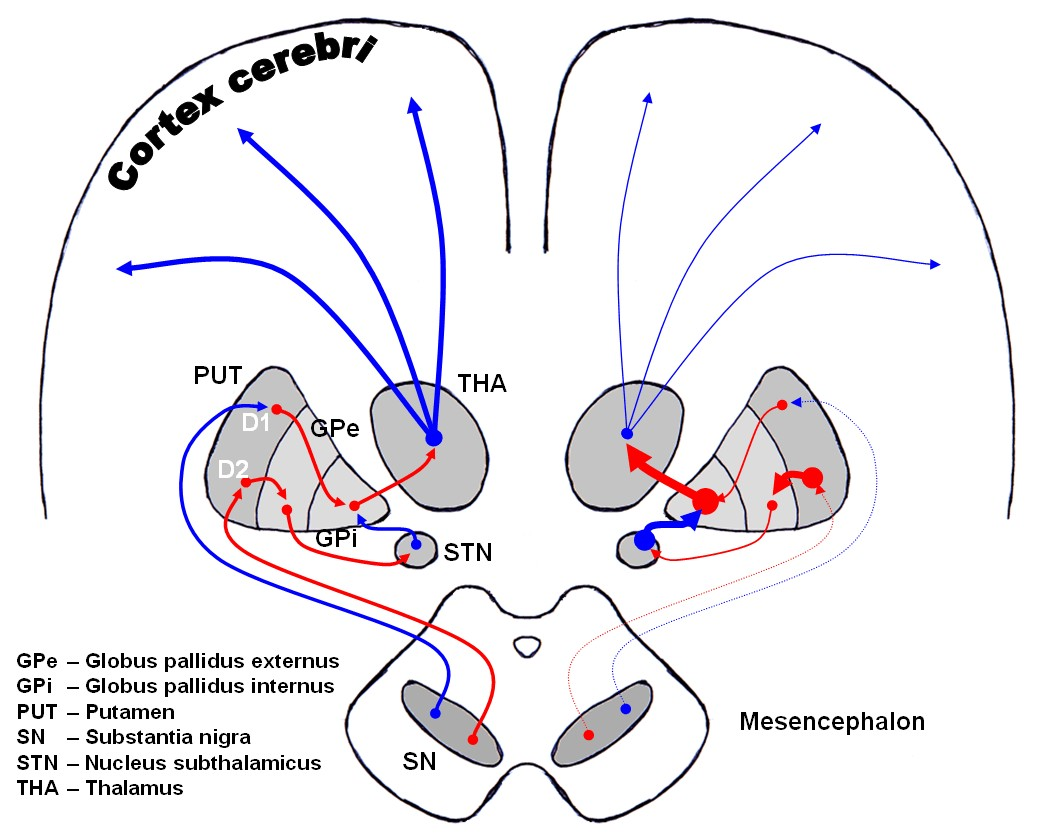
\includegraphics[width=0.5\linewidth]{FileAusiliari/Immagini/degenerative/dopamine-in-parkinsons-disease-illustration}
	\caption[Vie dopaminergiche]{L'immagine mostra le vie dopaminergiche del cervello umano in condizioni normali (a sinistra) e nella malattia di Parkinson (a destra). Le frecce rosse indicano la soppressione del bersaglio, quelle blu la stimolazione della struttura bersaglio. Caso per gentile concessione di Wikipedia, Radiopaedia.org, rID: 36286}
	\label{fig:dopamine-in-parkinsons-disease-illustration}
\end{figure*}

\subsection{Epidemiologia}
Il MP costituisce una delle principali cause di disabilità e mortalità nell'ambito delle patologie neurologiche, con una prevalenza particolarmente elevata negli Stati Uniti e in Canada (160-180 casi/100.000 abitanti). L'incidenza annuale in Nord America oscilla tra 108 e 212 casi ogni 100.000 individui di età $\geq$65 anni, con una prevalenza dello 0,3\% nella popolazione adulta $\geq$40 anni e dell'1,6\% nei soggetti ultrasessantacinquenni.
L'esordio della patologia mostra una significativa correlazione con l'età, manifestandosi tipicamente dalla quinta decade di vita, con un'età media alla diagnosi di 70,5 anni e una finestra di esordio prevalente tra i 45 e i 70 anni. Una variante giovanile può presentarsi tra i 20 e i 40 anni, sebbene l'esordio prima dei 30 anni risulti infrequente. La distribuzione per sesso evidenzia una predominanza maschile, particolarmente accentuata nella fascia d'età 50-60 anni.
L'eziologia del MP comprende fattori di rischio genetici, con particolare rilevanza nelle forme ad esordio precoce, e ambientali, tra cui l'esposizione a pesticidi e inquinanti atmosferici. Sono stati identificati fattori protettivi, inclusi il consumo di caffè, l'attività fisica e il fumo di sigaretta. La patologia si presenta prevalentemente in forma sporadica (85-90\% dei casi), mentre una minoranza dei casi (10-15\%) presenta familiarità positiva.

\subsubsection{Fattori di rischio}
L'eziopatogenesi del Morbo di Parkinson (MP) presenta una complessa interazione di fattori di rischio genetici, ambientali e non modificabili. L'anamnesi familiare positiva per MP in consanguinei di primo grado comporta un incremento del rischio relativo di 2-3 volte. Le forme monogeniche, rappresentanti meno del 10\% della casistica totale, manifestano pattern di ereditarietà autosomica dominante, recessiva o X-linked, caratterizzandosi per un esordio precoce rispetto alle forme sporadiche.
Le mutazioni eterozigoti del gene GBA1 costituiscono un significativo fattore di rischio genetico, unitamente ad alterazioni di altri geni codificanti per enzimi lisosomiali. Il coinvolgimento di geni quali SNCA, LRRK2, VPS35, Parkin, PINK1 e DJ-1 è stato ampiamente documentato. Particolare rilevanza assumono le mutazioni del gene Nurr1, determinante per l'identità neuronale dopaminergica, e del gene DJ-1, cruciale nella risposta allo stress ossidativo. Le alterazioni del gene PINK1, codificante per una chinasi mitocondriale, e del gene Park2, responsabile della sintesi della proteina parkina, sono associate a forme ad esordio precoce.
L'esposizione a neurotossine ambientali, inclusi mercurio, manganese, disolfuro di carbonio, solventi organici, MPTP e monossido di carbonio, può indurre degenerazione nigrostriatale e parkinsonismo. L'uso di neurolettici e l'abuso endovenoso di efedrone possono causare sindromi parkinsoniane potenzialmente irreversibili. Traumi cranici ripetuti, pesticidi, solventi e inquinamento atmosferico rappresentano ulteriori fattori di rischio ambientale documentati.
Tra i fattori non modificabili, l'età avanzata e il sesso maschile emergono come significativi predittori di rischio, con predominanza nella sesta decade di vita. Comorbidità quali depressione, ansia, stipsi, diabete mellito tipo 2, obesità e alterazioni del metabolismo del ferro sono state correlate a un incrementato rischio di MP.
Il consumo di tabacco e caffè, unitamente all'attività fisica regolare, ha mostrato effetti protettivi, sebbene di modesta entità. È fondamentale sottolineare che la maggioranza dei casi di MP rimane idiopatica, suggerendo un'eziologia multifattoriale.

\subsection{Presentazione  clinica}
La sintomatologia del Morbo di Parkinson manifesta un quadro clinico caratterizzato da manifestazioni motorie cardinali e sintomatologia non motoria associata. Il complesso sintomatologico motorio comprende tremore a riposo spesso asimmetrico con frequenza di 4-6 Hz, tipicamente descritto come "pill-rolling", bradicinesia manifestantesi con rallentamento motorio, ipomimia e ridotta oscillazione pendolare degli arti superiori durante la deambulazione, rigidità muscolare ("lead-pipe" o fenomeno della ruota dentata), e instabilità posturale documentabile attraverso il test della retropulsione. La deambulazione risulta caratterizzata da una progressione a piccoli passi con tendenza allo strascicamento e ridotta oscillazione degli arti superiori.
La sintomatologia accessoria include disartria con eloquio esplosivo secondario a incoordinazione linguo-diaframmatica, movimenti involontari della lingua con conseguente difficoltà protrusiva, e incremento della frequenza di ammiccamento palpebrale, quest'ultimo in contrasto con quanto osservato nella corea di Huntington. La disfunzione autonomica, i disturbi olfattivi, la sintomatologia algica, le alterazioni sensitive e i disturbi timici costituiscono il corredo sintomatologico non motorio. Il deterioramento cognitivo, con particolare coinvolgimento delle funzioni attentive, può manifestarsi e progredire nel decorso della patologia.
La progressione temporale della malattia evidenzia un esordio tipicamente unilaterale con successiva bilateralizzazione, manifestandosi prevalentemente nella sesta decade di vita. La responsività alla terapia dopaminergica, in particolare alla levodopa, rappresenta un elemento caratteristico, sebbene il tremore possa risultare farmacoresistente, in contrasto con la significativa risposta della bradicinesia e della rigidità. La variabilità fenotipica interindividuale costituisce un elemento distintivo della patologia.

\subsection{Approccio diagnostico}
L'iter diagnostico della malattia di Parkinson si fonda primariamente sulla valutazione clinica, data l'assenza di biomarcatori patognomonici. La diagnosi richiede la documentazione di bradicinesia associata ad almeno un sintomo cardine tra tremore a riposo o rigidità, valutati mediante la scala MDS-UPDRS standardizzata.
L'approccio diagnostico contempla un'accurata anamnesi ed esame obiettivo neurologico, focalizzati sull'identificazione dei sintomi cardinali: bradicinesia, tremore a riposo (4-6 Hz) tipicamente asimmetrico, rigidità e instabilità posturale. La responsività alla terapia dopaminergica, particolarmente evidente per bradicinesia e rigidità, costituisce un elemento diagnostico supportivo significativo, mentre una mancata risposta a dosaggi adeguati di levodopa suggerisce diagnosi alternative.
L'esclusione di parkinsonismi secondari richiede particolare attenzione all'insorgenza temporale dei sintomi e alla distribuzione topografica del coinvolgimento motorio. La diagnostica per immagini, sebbene non necessaria nelle presentazioni cliniche tipiche con adeguata risposta alla levodopa, può includere RM cerebrale, particolarmente utile mediante sequenze SWI per la valutazione del "swallow tail sign" nigrostriatale. La SPECT con 123I-FP-CIT (DaTscan) documenta la disfunzione dopaminergica presinaptica, mentre la PET con FDG consente la differenziazione metabolica tra PD e sindromi parkinsoniane atipiche.
L'analisi genetica, indicata in casi selezionati (esordio precoce, familiarità positiva, specifiche etnie), e la valutazione autonomica mediante scintigrafia miocardica con MIBG, che evidenzia la denervazione simpatica caratteristica, completano l'iter diagnostico. L'ecografia transcranica può evidenziare l'iperecogenicità della sostanza nera, supportando la diagnosi differenziale.
I criteri MDS stratificano la diagnosi in PD clinicamente stabilita e probabile, bilanciando specificità e sensibilità diagnostica nella pratica clinica.

\begin{Oss}
	La scala MDS-UPDRS (Movement Disorder Society-Unified Parkinson's Disease Rating Scale) è uno strumento di valutazione clinica ampiamente utilizzato per quantificare la gravità dei sintomi motori e non motori della malattia di Parkinson. Questa scala è stata sviluppata per migliorare la consistenza nella valutazione dei sintomi e per integrare meglio gli aspetti non motori della PD.
	Struttura: La scala MDS-UPDRS è composta da quattro sezioni:
	\begin{description}
		\item[Sezione I]{Esperienze non motorie della vita quotidiana. Questa sezione valuta aspetti come le capacità cognitive, i disturbi comportamentali e dell'umore}
		\item [Sezione II]{Esperienze motorie della vita quotidiana. Questa sezione valuta l'impatto dei sintomi motori sulle attività quotidiane}
		\item [Sezione III]{Esame motorio. Questa sezione valuta i segni motori della PD attraverso un esame clinico, come il tremore, la rigidità e la bradicinesia}
		\item[Sezione IV]{Complicanze della terapia. Questa sezione valuta le complicanze associate al trattamento farmacologico}
	\end{description}
	Il punteggio totale per le sezioni I-IV varia da 0 (nessuna disabilità) a 199 (disabilità totale). La sezione III, che valuta i sintomi motori, ha un punteggio che varia da 0 a 132.
	Oltre alla scala MDS-UPDRS, esistono altre scale di valutazione utilizzate nella PD, come la scala di Hoehn e Yahr e la scala di Schwab e England. La scala di Hoehn e Yahr valuta la gravità della malattia da 0 (nessuna malattia) a 5 (paziente costretto su sedia a rotelle o allettato senza assistenza).
\end{Oss}

\subsection{Anatomia patologica}
Dal punto di vista anatomopatologico il morbo di Parkinson si manifesta attraverso inclusioni proteiche intraneuronali denominate corpi di Lewy, costituiti primariamente da aggregati patologici di alfa-sinucleina, una proteina sinaptica fisiologicamente presente nel sistema nervoso centrale. L'accumulo di queste inclusioni, sebbene non patognomonico del morbo di Parkinson essendo documentabile anche nella demenza a corpi di Lewy, rappresenta una caratteristica istopatologica fondamentale quando localizzato nella substantia nigra, in associazione alla perdita neuronale dopaminergica. L'assenza di corpi di Lewy nelle forme post-encefalitiche, caratterizzate invece da grovigli neurofibrillari, e in alcune forme geneticamente determinate, sottolinea l'eterogeneità patogenetica della malattia.
La progressione spazio-temporale della patologia, codificata nello staging di Braak, delinea sei stadi evolutivi caratterizzati da una diffusione ascendente delle alterazioni neuropatologiche. Gli stadi iniziali (1-2) coinvolgono il nucleo motore dorsale dei nervi glossofaringeo e vago e il nucleo olfattivo anteriore, precedendo frequentemente la sintomatologia motoria. Gli stadi intermedi (3-4) documentano il coinvolgimento della substantia nigra pars compacta, del prosencefalo basale e della mesocorteccia temporale, correlando con l'esordio clinico della malattia. Gli stadi terminali (5-6) evidenziano una progressione neocorticale diffusa.
La patogenesi molecolare implica alterazioni del metabolismo dell'alfa-sinucleina, potenzialmente accelerate da disfunzioni delle proteine heat shock o dall'azione della dopamina. Il coinvolgimento della proteina parkin nella degradazione proteasomica evidenzia meccanismi neurodegenerativi potenzialmente indipendenti dalla formazione dei corpi di Lewy.
L'alfa-sinucleina, proteina fisiologicamente localizzata nelle terminazioni presinaptiche neuronali, manifesta nella patogenesi del morbo di Parkinson un processo patologico caratterizzato da misfolding proteico e successiva aggregazione in oligomeri, protofibrille e fibrille, culminante nella formazione dei corpi di Lewy intraneuronali. Questi aggregati proteici, considerati hallmark istopatologico della malattia, evidenziano particolare neurotossicità nella forma protofibrillare, determinando disfunzione e successiva degenerazione neuronale dopaminergica nigrostriatale.
L'identificazione di mutazioni nel gene SNCA, codificante per l'alfa-sinucleina, nelle forme familiari di malattia, unitamente alla documentazione di fenotipi clinici particolarmente aggressivi in presenza di duplicazione o triplicazione genica, ha fornito evidenze significative del ruolo causale di questa proteina nella patogenesi della malattia. La documentata capacità di trasmissione transcellulare dell'alfa-sinucleina patologica costituisce il substrato molecolare della progressione anatomopatologica descritta nello staging di Braak.
La disfunzione sinaptica correlata all'accumulo di alfa-sinucleina rappresenta un meccanismo patogenetico critico, modulato da fattori quali stress ossidativo, alterazioni del sistema ubiquitina-proteasoma e interazione con il metabolismo dopaminergico. Mutazioni nei geni parkin, PINK1 e DJ-1 influenzano il metabolismo dell'alfa-sinucleina attraverso alterazioni dei sistemi di degradazione proteica.
L'alfa-sinucleina costituisce attualmente un promettente target terapeutico, con particolare interesse per lo sviluppo di anticorpi monoclonali specifici e inibitori dell'aggregazione proteica, finalizzati al rallentamento della progressione patologica.

\subsection{Imaging}

\subsubsection{TC}
La TC manifesta un'utilità clinica circoscritta nella valutazione diagnostica primaria del MP, assumendo rilevanza nell'esclusione di patologie strutturali mimiche quali lesioni espansive, idrocefalo o alterazioni vascolari, particolarmente in presenza di presentazioni cliniche atipiche o "red flags" suggestive di diagnosi alternative.
Nel contesto della gestione terapeutica, la TC assume particolare rilevanza nella valutazione post-chirurgica della stimolazione cerebrale profonda (DBS), consentendo la verifica del corretto posizionamento degli elettrodi nel nucleo subtalamico (STN), tipicamente localizzati a 9mm dalla linea mediana, e l'identificazione di eventuali complicanze post-procedurali quali eventi emorragici, ischemici o fenomeni infiammatori transitori, questi ultimi caratterizzati da aree ipodense perilettrodiche a risoluzione graduale. L'utilità della metodica nel follow-up routinario post-DBS risulta secondaria.
La sensibilità subottimale della TC nella diagnosi differenziale tra PD e sindromi parkinsoniane atipiche, incluse atrofia multisistemica e paralisi sopranucleare progressiva, nonché nella distinzione dal tremore essenziale, ne limita significativamente l'applicazione clinica in questo contesto diagnostico.

\subsubsection{RM}
La RM è frequentemente normale nelle sequenze convenzionali (T1, T2, FLAIR) nelle fasi iniziali di malattia. L'implementazione di sequenze susceptibility-weighted imaging (SWI) o T2*-weighted ad alta risoluzione consente la visualizzazione del nigrosoma-1, struttura caratterizzata dal patognomonico "swallow tail sign", la cui perdita correla con la degenerazione dopaminergica nigrostriatale. L'accumulo patologico di ferro nella substantia nigra, quantificabile mediante sequenze SWI/T2* e incrementato del 50\% rispetto ai controlli, costituisce un ulteriore marker diagnostico, complementato dall'imaging della neuromelanina mediante sequenze T1 con impulsi di trasferimento di magnetizzazione (MTC).

\begin{figure*}[h]
	\centering
	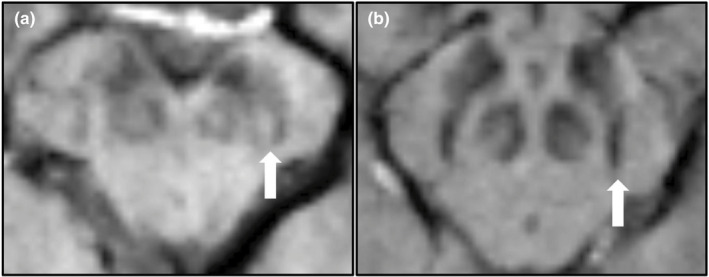
\includegraphics[width=0.8\linewidth]{FileAusiliari/Immagini/degenerative/BRB3-11-e02202-g002}
	\caption{Esempi di segno della coda di rondine (STS) in un individuo malato (a) e di STS assente in un individuo sano (b). Sono mostrate sezioni assiali del mesencefalo mappate tramite imaging pesato con suscettibilità (SWI). Le frecce bianche indicano la diversa configurazione del Nigrosoma-1 (N1). Da Brain Behav. 2021 May 24;11(7):e02202. doi: 10.1002/brb3.2202}
	\label{fig:brb3-11-e02202-g002}
\end{figure*}


La diagnosi differenziale delle sindromi parkinsoniane atipiche beneficia significativamente dell'imaging RM. L'atrofia multisistemica (MSA) evidenzia caratteristica atrofia putaminale, pontica e cerebellare, con ipointensità putaminale T2/SWI e "hot cross bun sign" pontino. La paralisi sopranucleare progressiva (PSP) manifesta atrofia mesencefalica con alterazione del rapporto mesencefalo-ponte, mentre la degenerazione corticobasale (CBD) presenta atrofia frontoparietale asimmetrica con iperintensità della sostanza bianca subcorticale.
Metodiche avanzate quali Diffusion Tensor Imaging (DTI) e risonanza magnetica funzionale (fMRI) consentono la caratterizzazione delle alterazioni microstrutturali della sostanza bianca e delle modificazioni funzionali cerebrali, sebbene la sensibilità nell'identificazione della progressione patologica e nella valutazione della risposta terapeutica necessiti ulteriore validazione. Le limitazioni metodologiche includono variabilità interindividuale e sovrapposizione dei reperti radiologici nelle diverse sindromi parkinsoniane.

\subsection{Trattamento e prognosi}

\subsection{Checklist di refertazione}

\begin{itemize}[label=$\square$] % Riquadro vuoto come simbolo
	\item Escludi altre cause di parkinsonismo (es ictus)
	\item Controlla il segnale dei nigrosomi
	\item Controlla il trofismo delle strutture sottotentoriali
\end{itemize}

\subsection{Bibliografia}
\small{
	
	
}

\note{Nota a margine}
\expl{Nota a margine colorata}
\input{Capitoli/vascolare/stroke_ischemico.tex}
\input{Capitoli/vascolare/patologia_vascolare.tex}
\input{Capitoli/vascolare/malattia_piccoli_vasi.tex}
\input{Capitoli/vascolare/emorragie_intraparenchimali.tex}
\input{Capitoli/vascolare/emorragia_subaracnoidea.tex}
\input{Capitoli/vascolare/trombosi_venosa.tex}
\input{Capitoli/degenerative/approccio.tex}
\input{Capitoli/degenerative/degenerative.tex}
\section{Morbo di Parkinson}

\subsection{Definizione}

\subsection{Eziologia}

\begin{figure*}[h]
	\centering
	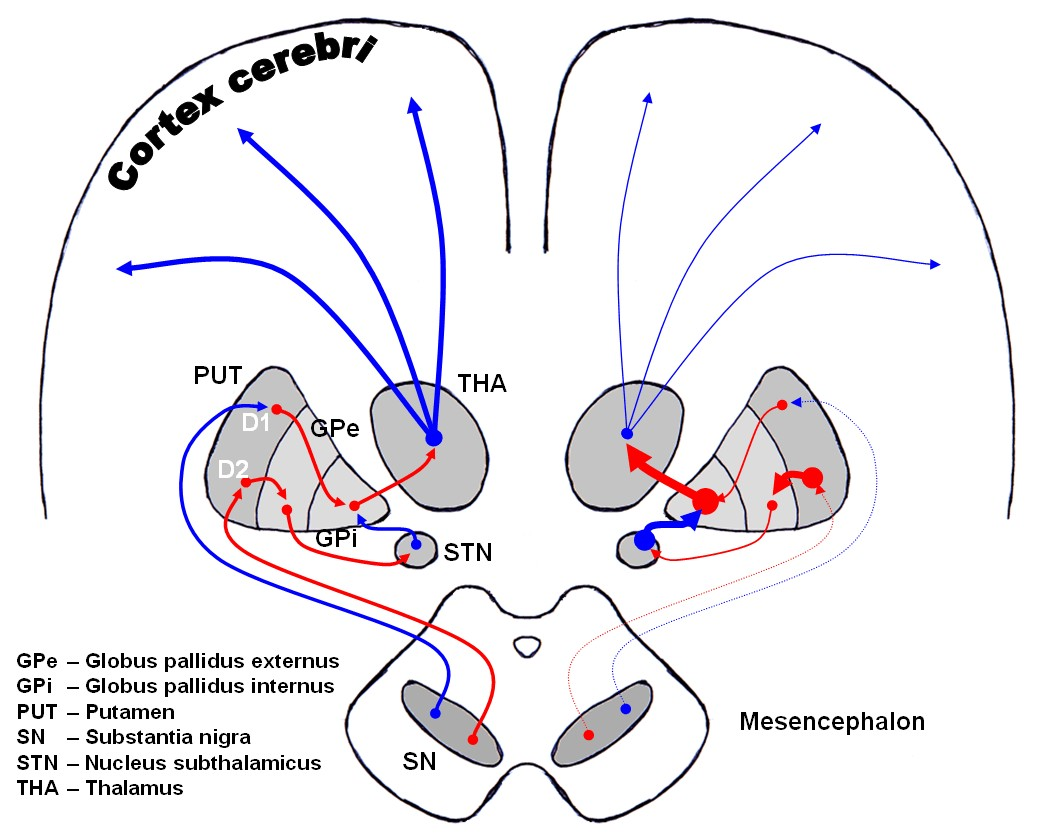
\includegraphics[width=0.5\linewidth]{FileAusiliari/Immagini/degenerative/dopamine-in-parkinsons-disease-illustration}
	\caption[Vie dopaminergiche]{L'immagine mostra le vie dopaminergiche del cervello umano in condizioni normali (a sinistra) e nella malattia di Parkinson (a destra). Le frecce rosse indicano la soppressione del bersaglio, quelle blu la stimolazione della struttura bersaglio. Caso per gentile concessione di Wikipedia, Radiopaedia.org, rID: 36286}
	\label{fig:dopamine-in-parkinsons-disease-illustration}
\end{figure*}

\subsection{Epidemiologia}
Il MP costituisce una delle principali cause di disabilità e mortalità nell'ambito delle patologie neurologiche, con una prevalenza particolarmente elevata negli Stati Uniti e in Canada (160-180 casi/100.000 abitanti). L'incidenza annuale in Nord America oscilla tra 108 e 212 casi ogni 100.000 individui di età $\geq$65 anni, con una prevalenza dello 0,3\% nella popolazione adulta $\geq$40 anni e dell'1,6\% nei soggetti ultrasessantacinquenni.
L'esordio della patologia mostra una significativa correlazione con l'età, manifestandosi tipicamente dalla quinta decade di vita, con un'età media alla diagnosi di 70,5 anni e una finestra di esordio prevalente tra i 45 e i 70 anni. Una variante giovanile può presentarsi tra i 20 e i 40 anni, sebbene l'esordio prima dei 30 anni risulti infrequente. La distribuzione per sesso evidenzia una predominanza maschile, particolarmente accentuata nella fascia d'età 50-60 anni.
L'eziologia del MP comprende fattori di rischio genetici, con particolare rilevanza nelle forme ad esordio precoce, e ambientali, tra cui l'esposizione a pesticidi e inquinanti atmosferici. Sono stati identificati fattori protettivi, inclusi il consumo di caffè, l'attività fisica e il fumo di sigaretta. La patologia si presenta prevalentemente in forma sporadica (85-90\% dei casi), mentre una minoranza dei casi (10-15\%) presenta familiarità positiva.

\subsubsection{Fattori di rischio}
L'eziopatogenesi del Morbo di Parkinson (MP) presenta una complessa interazione di fattori di rischio genetici, ambientali e non modificabili. L'anamnesi familiare positiva per MP in consanguinei di primo grado comporta un incremento del rischio relativo di 2-3 volte. Le forme monogeniche, rappresentanti meno del 10\% della casistica totale, manifestano pattern di ereditarietà autosomica dominante, recessiva o X-linked, caratterizzandosi per un esordio precoce rispetto alle forme sporadiche.
Le mutazioni eterozigoti del gene GBA1 costituiscono un significativo fattore di rischio genetico, unitamente ad alterazioni di altri geni codificanti per enzimi lisosomiali. Il coinvolgimento di geni quali SNCA, LRRK2, VPS35, Parkin, PINK1 e DJ-1 è stato ampiamente documentato. Particolare rilevanza assumono le mutazioni del gene Nurr1, determinante per l'identità neuronale dopaminergica, e del gene DJ-1, cruciale nella risposta allo stress ossidativo. Le alterazioni del gene PINK1, codificante per una chinasi mitocondriale, e del gene Park2, responsabile della sintesi della proteina parkina, sono associate a forme ad esordio precoce.
L'esposizione a neurotossine ambientali, inclusi mercurio, manganese, disolfuro di carbonio, solventi organici, MPTP e monossido di carbonio, può indurre degenerazione nigrostriatale e parkinsonismo. L'uso di neurolettici e l'abuso endovenoso di efedrone possono causare sindromi parkinsoniane potenzialmente irreversibili. Traumi cranici ripetuti, pesticidi, solventi e inquinamento atmosferico rappresentano ulteriori fattori di rischio ambientale documentati.
Tra i fattori non modificabili, l'età avanzata e il sesso maschile emergono come significativi predittori di rischio, con predominanza nella sesta decade di vita. Comorbidità quali depressione, ansia, stipsi, diabete mellito tipo 2, obesità e alterazioni del metabolismo del ferro sono state correlate a un incrementato rischio di MP.
Il consumo di tabacco e caffè, unitamente all'attività fisica regolare, ha mostrato effetti protettivi, sebbene di modesta entità. È fondamentale sottolineare che la maggioranza dei casi di MP rimane idiopatica, suggerendo un'eziologia multifattoriale.

\subsection{Presentazione  clinica}
La sintomatologia del Morbo di Parkinson manifesta un quadro clinico caratterizzato da manifestazioni motorie cardinali e sintomatologia non motoria associata. Il complesso sintomatologico motorio comprende tremore a riposo spesso asimmetrico con frequenza di 4-6 Hz, tipicamente descritto come "pill-rolling", bradicinesia manifestantesi con rallentamento motorio, ipomimia e ridotta oscillazione pendolare degli arti superiori durante la deambulazione, rigidità muscolare ("lead-pipe" o fenomeno della ruota dentata), e instabilità posturale documentabile attraverso il test della retropulsione. La deambulazione risulta caratterizzata da una progressione a piccoli passi con tendenza allo strascicamento e ridotta oscillazione degli arti superiori.
La sintomatologia accessoria include disartria con eloquio esplosivo secondario a incoordinazione linguo-diaframmatica, movimenti involontari della lingua con conseguente difficoltà protrusiva, e incremento della frequenza di ammiccamento palpebrale, quest'ultimo in contrasto con quanto osservato nella corea di Huntington. La disfunzione autonomica, i disturbi olfattivi, la sintomatologia algica, le alterazioni sensitive e i disturbi timici costituiscono il corredo sintomatologico non motorio. Il deterioramento cognitivo, con particolare coinvolgimento delle funzioni attentive, può manifestarsi e progredire nel decorso della patologia.
La progressione temporale della malattia evidenzia un esordio tipicamente unilaterale con successiva bilateralizzazione, manifestandosi prevalentemente nella sesta decade di vita. La responsività alla terapia dopaminergica, in particolare alla levodopa, rappresenta un elemento caratteristico, sebbene il tremore possa risultare farmacoresistente, in contrasto con la significativa risposta della bradicinesia e della rigidità. La variabilità fenotipica interindividuale costituisce un elemento distintivo della patologia.

\subsection{Approccio diagnostico}
L'iter diagnostico della malattia di Parkinson si fonda primariamente sulla valutazione clinica, data l'assenza di biomarcatori patognomonici. La diagnosi richiede la documentazione di bradicinesia associata ad almeno un sintomo cardine tra tremore a riposo o rigidità, valutati mediante la scala MDS-UPDRS standardizzata.
L'approccio diagnostico contempla un'accurata anamnesi ed esame obiettivo neurologico, focalizzati sull'identificazione dei sintomi cardinali: bradicinesia, tremore a riposo (4-6 Hz) tipicamente asimmetrico, rigidità e instabilità posturale. La responsività alla terapia dopaminergica, particolarmente evidente per bradicinesia e rigidità, costituisce un elemento diagnostico supportivo significativo, mentre una mancata risposta a dosaggi adeguati di levodopa suggerisce diagnosi alternative.
L'esclusione di parkinsonismi secondari richiede particolare attenzione all'insorgenza temporale dei sintomi e alla distribuzione topografica del coinvolgimento motorio. La diagnostica per immagini, sebbene non necessaria nelle presentazioni cliniche tipiche con adeguata risposta alla levodopa, può includere RM cerebrale, particolarmente utile mediante sequenze SWI per la valutazione del "swallow tail sign" nigrostriatale. La SPECT con 123I-FP-CIT (DaTscan) documenta la disfunzione dopaminergica presinaptica, mentre la PET con FDG consente la differenziazione metabolica tra PD e sindromi parkinsoniane atipiche.
L'analisi genetica, indicata in casi selezionati (esordio precoce, familiarità positiva, specifiche etnie), e la valutazione autonomica mediante scintigrafia miocardica con MIBG, che evidenzia la denervazione simpatica caratteristica, completano l'iter diagnostico. L'ecografia transcranica può evidenziare l'iperecogenicità della sostanza nera, supportando la diagnosi differenziale.
I criteri MDS stratificano la diagnosi in PD clinicamente stabilita e probabile, bilanciando specificità e sensibilità diagnostica nella pratica clinica.

\begin{Oss}
	La scala MDS-UPDRS (Movement Disorder Society-Unified Parkinson's Disease Rating Scale) è uno strumento di valutazione clinica ampiamente utilizzato per quantificare la gravità dei sintomi motori e non motori della malattia di Parkinson. Questa scala è stata sviluppata per migliorare la consistenza nella valutazione dei sintomi e per integrare meglio gli aspetti non motori della PD.
	Struttura: La scala MDS-UPDRS è composta da quattro sezioni:
	\begin{description}
		\item[Sezione I]{Esperienze non motorie della vita quotidiana. Questa sezione valuta aspetti come le capacità cognitive, i disturbi comportamentali e dell'umore}
		\item [Sezione II]{Esperienze motorie della vita quotidiana. Questa sezione valuta l'impatto dei sintomi motori sulle attività quotidiane}
		\item [Sezione III]{Esame motorio. Questa sezione valuta i segni motori della PD attraverso un esame clinico, come il tremore, la rigidità e la bradicinesia}
		\item[Sezione IV]{Complicanze della terapia. Questa sezione valuta le complicanze associate al trattamento farmacologico}
	\end{description}
	Il punteggio totale per le sezioni I-IV varia da 0 (nessuna disabilità) a 199 (disabilità totale). La sezione III, che valuta i sintomi motori, ha un punteggio che varia da 0 a 132.
	Oltre alla scala MDS-UPDRS, esistono altre scale di valutazione utilizzate nella PD, come la scala di Hoehn e Yahr e la scala di Schwab e England. La scala di Hoehn e Yahr valuta la gravità della malattia da 0 (nessuna malattia) a 5 (paziente costretto su sedia a rotelle o allettato senza assistenza).
\end{Oss}

\subsection{Anatomia patologica}
Dal punto di vista anatomopatologico il morbo di Parkinson si manifesta attraverso inclusioni proteiche intraneuronali denominate corpi di Lewy, costituiti primariamente da aggregati patologici di alfa-sinucleina, una proteina sinaptica fisiologicamente presente nel sistema nervoso centrale. L'accumulo di queste inclusioni, sebbene non patognomonico del morbo di Parkinson essendo documentabile anche nella demenza a corpi di Lewy, rappresenta una caratteristica istopatologica fondamentale quando localizzato nella substantia nigra, in associazione alla perdita neuronale dopaminergica. L'assenza di corpi di Lewy nelle forme post-encefalitiche, caratterizzate invece da grovigli neurofibrillari, e in alcune forme geneticamente determinate, sottolinea l'eterogeneità patogenetica della malattia.
La progressione spazio-temporale della patologia, codificata nello staging di Braak, delinea sei stadi evolutivi caratterizzati da una diffusione ascendente delle alterazioni neuropatologiche. Gli stadi iniziali (1-2) coinvolgono il nucleo motore dorsale dei nervi glossofaringeo e vago e il nucleo olfattivo anteriore, precedendo frequentemente la sintomatologia motoria. Gli stadi intermedi (3-4) documentano il coinvolgimento della substantia nigra pars compacta, del prosencefalo basale e della mesocorteccia temporale, correlando con l'esordio clinico della malattia. Gli stadi terminali (5-6) evidenziano una progressione neocorticale diffusa.
La patogenesi molecolare implica alterazioni del metabolismo dell'alfa-sinucleina, potenzialmente accelerate da disfunzioni delle proteine heat shock o dall'azione della dopamina. Il coinvolgimento della proteina parkin nella degradazione proteasomica evidenzia meccanismi neurodegenerativi potenzialmente indipendenti dalla formazione dei corpi di Lewy.
L'alfa-sinucleina, proteina fisiologicamente localizzata nelle terminazioni presinaptiche neuronali, manifesta nella patogenesi del morbo di Parkinson un processo patologico caratterizzato da misfolding proteico e successiva aggregazione in oligomeri, protofibrille e fibrille, culminante nella formazione dei corpi di Lewy intraneuronali. Questi aggregati proteici, considerati hallmark istopatologico della malattia, evidenziano particolare neurotossicità nella forma protofibrillare, determinando disfunzione e successiva degenerazione neuronale dopaminergica nigrostriatale.
L'identificazione di mutazioni nel gene SNCA, codificante per l'alfa-sinucleina, nelle forme familiari di malattia, unitamente alla documentazione di fenotipi clinici particolarmente aggressivi in presenza di duplicazione o triplicazione genica, ha fornito evidenze significative del ruolo causale di questa proteina nella patogenesi della malattia. La documentata capacità di trasmissione transcellulare dell'alfa-sinucleina patologica costituisce il substrato molecolare della progressione anatomopatologica descritta nello staging di Braak.
La disfunzione sinaptica correlata all'accumulo di alfa-sinucleina rappresenta un meccanismo patogenetico critico, modulato da fattori quali stress ossidativo, alterazioni del sistema ubiquitina-proteasoma e interazione con il metabolismo dopaminergico. Mutazioni nei geni parkin, PINK1 e DJ-1 influenzano il metabolismo dell'alfa-sinucleina attraverso alterazioni dei sistemi di degradazione proteica.
L'alfa-sinucleina costituisce attualmente un promettente target terapeutico, con particolare interesse per lo sviluppo di anticorpi monoclonali specifici e inibitori dell'aggregazione proteica, finalizzati al rallentamento della progressione patologica.

\subsection{Imaging}

\subsubsection{TC}
La TC manifesta un'utilità clinica circoscritta nella valutazione diagnostica primaria del MP, assumendo rilevanza nell'esclusione di patologie strutturali mimiche quali lesioni espansive, idrocefalo o alterazioni vascolari, particolarmente in presenza di presentazioni cliniche atipiche o "red flags" suggestive di diagnosi alternative.
Nel contesto della gestione terapeutica, la TC assume particolare rilevanza nella valutazione post-chirurgica della stimolazione cerebrale profonda (DBS), consentendo la verifica del corretto posizionamento degli elettrodi nel nucleo subtalamico (STN), tipicamente localizzati a 9mm dalla linea mediana, e l'identificazione di eventuali complicanze post-procedurali quali eventi emorragici, ischemici o fenomeni infiammatori transitori, questi ultimi caratterizzati da aree ipodense perilettrodiche a risoluzione graduale. L'utilità della metodica nel follow-up routinario post-DBS risulta secondaria.
La sensibilità subottimale della TC nella diagnosi differenziale tra PD e sindromi parkinsoniane atipiche, incluse atrofia multisistemica e paralisi sopranucleare progressiva, nonché nella distinzione dal tremore essenziale, ne limita significativamente l'applicazione clinica in questo contesto diagnostico.

\subsubsection{RM}
La RM è frequentemente normale nelle sequenze convenzionali (T1, T2, FLAIR) nelle fasi iniziali di malattia. L'implementazione di sequenze susceptibility-weighted imaging (SWI) o T2*-weighted ad alta risoluzione consente la visualizzazione del nigrosoma-1, struttura caratterizzata dal patognomonico "swallow tail sign", la cui perdita correla con la degenerazione dopaminergica nigrostriatale. L'accumulo patologico di ferro nella substantia nigra, quantificabile mediante sequenze SWI/T2* e incrementato del 50\% rispetto ai controlli, costituisce un ulteriore marker diagnostico, complementato dall'imaging della neuromelanina mediante sequenze T1 con impulsi di trasferimento di magnetizzazione (MTC).

\begin{figure*}[h]
	\centering
	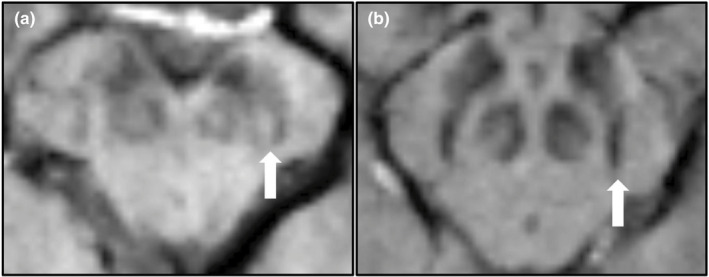
\includegraphics[width=0.8\linewidth]{FileAusiliari/Immagini/degenerative/BRB3-11-e02202-g002}
	\caption{Esempi di segno della coda di rondine (STS) in un individuo malato (a) e di STS assente in un individuo sano (b). Sono mostrate sezioni assiali del mesencefalo mappate tramite imaging pesato con suscettibilità (SWI). Le frecce bianche indicano la diversa configurazione del Nigrosoma-1 (N1). Da Brain Behav. 2021 May 24;11(7):e02202. doi: 10.1002/brb3.2202}
	\label{fig:brb3-11-e02202-g002}
\end{figure*}


La diagnosi differenziale delle sindromi parkinsoniane atipiche beneficia significativamente dell'imaging RM. L'atrofia multisistemica (MSA) evidenzia caratteristica atrofia putaminale, pontica e cerebellare, con ipointensità putaminale T2/SWI e "hot cross bun sign" pontino. La paralisi sopranucleare progressiva (PSP) manifesta atrofia mesencefalica con alterazione del rapporto mesencefalo-ponte, mentre la degenerazione corticobasale (CBD) presenta atrofia frontoparietale asimmetrica con iperintensità della sostanza bianca subcorticale.
Metodiche avanzate quali Diffusion Tensor Imaging (DTI) e risonanza magnetica funzionale (fMRI) consentono la caratterizzazione delle alterazioni microstrutturali della sostanza bianca e delle modificazioni funzionali cerebrali, sebbene la sensibilità nell'identificazione della progressione patologica e nella valutazione della risposta terapeutica necessiti ulteriore validazione. Le limitazioni metodologiche includono variabilità interindividuale e sovrapposizione dei reperti radiologici nelle diverse sindromi parkinsoniane.

\subsection{Trattamento e prognosi}

\subsection{Checklist di refertazione}

\begin{itemize}[label=$\square$] % Riquadro vuoto come simbolo
	\item Escludi altre cause di parkinsonismo (es ictus)
	\item Controlla il segnale dei nigrosomi
	\item Controlla il trofismo delle strutture sottotentoriali
\end{itemize}

\subsection{Bibliografia}
\small{
	
	
}

\note{Nota a margine}
\expl{Nota a margine colorata}
\input{Capitoli/degenerative/approccio.tex}
\input{Capitoli/degenerative/degenerative.tex}
\section{Morbo di Parkinson}

\subsection{Definizione}

\subsection{Eziologia}

\begin{figure*}[h]
	\centering
	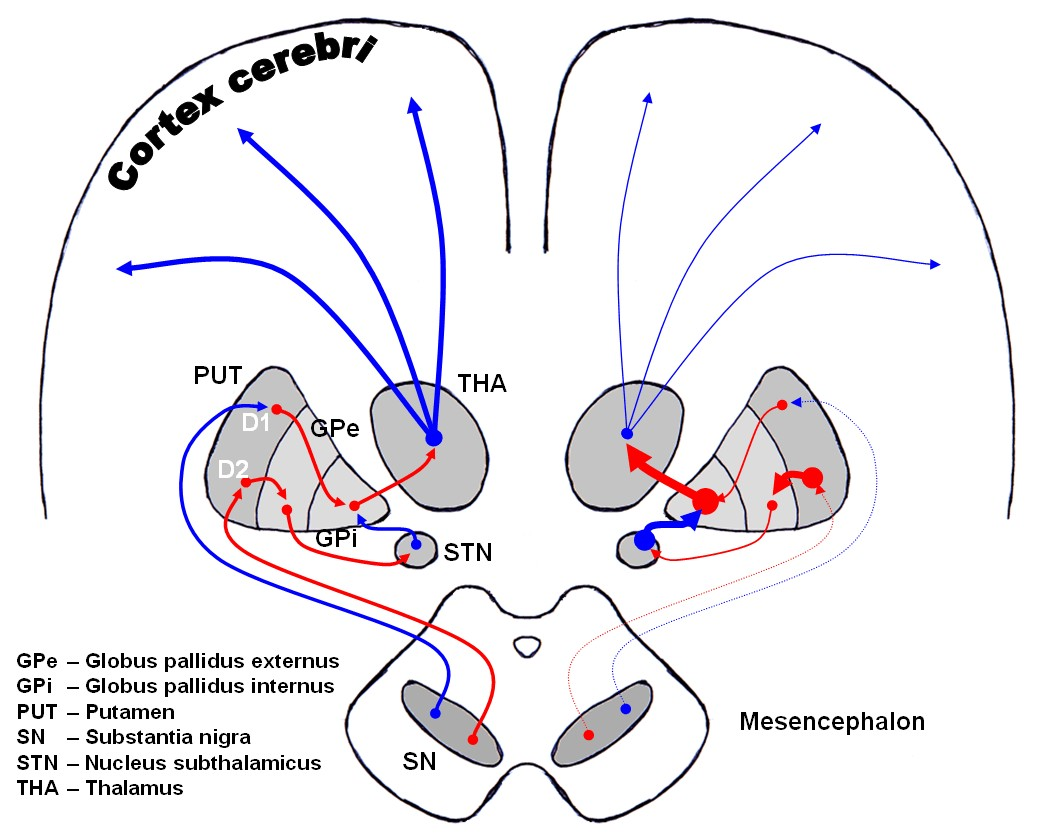
\includegraphics[width=0.5\linewidth]{FileAusiliari/Immagini/degenerative/dopamine-in-parkinsons-disease-illustration}
	\caption[Vie dopaminergiche]{L'immagine mostra le vie dopaminergiche del cervello umano in condizioni normali (a sinistra) e nella malattia di Parkinson (a destra). Le frecce rosse indicano la soppressione del bersaglio, quelle blu la stimolazione della struttura bersaglio. Caso per gentile concessione di Wikipedia, Radiopaedia.org, rID: 36286}
	\label{fig:dopamine-in-parkinsons-disease-illustration}
\end{figure*}

\subsection{Epidemiologia}
Il MP costituisce una delle principali cause di disabilità e mortalità nell'ambito delle patologie neurologiche, con una prevalenza particolarmente elevata negli Stati Uniti e in Canada (160-180 casi/100.000 abitanti). L'incidenza annuale in Nord America oscilla tra 108 e 212 casi ogni 100.000 individui di età $\geq$65 anni, con una prevalenza dello 0,3\% nella popolazione adulta $\geq$40 anni e dell'1,6\% nei soggetti ultrasessantacinquenni.
L'esordio della patologia mostra una significativa correlazione con l'età, manifestandosi tipicamente dalla quinta decade di vita, con un'età media alla diagnosi di 70,5 anni e una finestra di esordio prevalente tra i 45 e i 70 anni. Una variante giovanile può presentarsi tra i 20 e i 40 anni, sebbene l'esordio prima dei 30 anni risulti infrequente. La distribuzione per sesso evidenzia una predominanza maschile, particolarmente accentuata nella fascia d'età 50-60 anni.
L'eziologia del MP comprende fattori di rischio genetici, con particolare rilevanza nelle forme ad esordio precoce, e ambientali, tra cui l'esposizione a pesticidi e inquinanti atmosferici. Sono stati identificati fattori protettivi, inclusi il consumo di caffè, l'attività fisica e il fumo di sigaretta. La patologia si presenta prevalentemente in forma sporadica (85-90\% dei casi), mentre una minoranza dei casi (10-15\%) presenta familiarità positiva.

\subsubsection{Fattori di rischio}
L'eziopatogenesi del Morbo di Parkinson (MP) presenta una complessa interazione di fattori di rischio genetici, ambientali e non modificabili. L'anamnesi familiare positiva per MP in consanguinei di primo grado comporta un incremento del rischio relativo di 2-3 volte. Le forme monogeniche, rappresentanti meno del 10\% della casistica totale, manifestano pattern di ereditarietà autosomica dominante, recessiva o X-linked, caratterizzandosi per un esordio precoce rispetto alle forme sporadiche.
Le mutazioni eterozigoti del gene GBA1 costituiscono un significativo fattore di rischio genetico, unitamente ad alterazioni di altri geni codificanti per enzimi lisosomiali. Il coinvolgimento di geni quali SNCA, LRRK2, VPS35, Parkin, PINK1 e DJ-1 è stato ampiamente documentato. Particolare rilevanza assumono le mutazioni del gene Nurr1, determinante per l'identità neuronale dopaminergica, e del gene DJ-1, cruciale nella risposta allo stress ossidativo. Le alterazioni del gene PINK1, codificante per una chinasi mitocondriale, e del gene Park2, responsabile della sintesi della proteina parkina, sono associate a forme ad esordio precoce.
L'esposizione a neurotossine ambientali, inclusi mercurio, manganese, disolfuro di carbonio, solventi organici, MPTP e monossido di carbonio, può indurre degenerazione nigrostriatale e parkinsonismo. L'uso di neurolettici e l'abuso endovenoso di efedrone possono causare sindromi parkinsoniane potenzialmente irreversibili. Traumi cranici ripetuti, pesticidi, solventi e inquinamento atmosferico rappresentano ulteriori fattori di rischio ambientale documentati.
Tra i fattori non modificabili, l'età avanzata e il sesso maschile emergono come significativi predittori di rischio, con predominanza nella sesta decade di vita. Comorbidità quali depressione, ansia, stipsi, diabete mellito tipo 2, obesità e alterazioni del metabolismo del ferro sono state correlate a un incrementato rischio di MP.
Il consumo di tabacco e caffè, unitamente all'attività fisica regolare, ha mostrato effetti protettivi, sebbene di modesta entità. È fondamentale sottolineare che la maggioranza dei casi di MP rimane idiopatica, suggerendo un'eziologia multifattoriale.

\subsection{Presentazione  clinica}
La sintomatologia del Morbo di Parkinson manifesta un quadro clinico caratterizzato da manifestazioni motorie cardinali e sintomatologia non motoria associata. Il complesso sintomatologico motorio comprende tremore a riposo spesso asimmetrico con frequenza di 4-6 Hz, tipicamente descritto come "pill-rolling", bradicinesia manifestantesi con rallentamento motorio, ipomimia e ridotta oscillazione pendolare degli arti superiori durante la deambulazione, rigidità muscolare ("lead-pipe" o fenomeno della ruota dentata), e instabilità posturale documentabile attraverso il test della retropulsione. La deambulazione risulta caratterizzata da una progressione a piccoli passi con tendenza allo strascicamento e ridotta oscillazione degli arti superiori.
La sintomatologia accessoria include disartria con eloquio esplosivo secondario a incoordinazione linguo-diaframmatica, movimenti involontari della lingua con conseguente difficoltà protrusiva, e incremento della frequenza di ammiccamento palpebrale, quest'ultimo in contrasto con quanto osservato nella corea di Huntington. La disfunzione autonomica, i disturbi olfattivi, la sintomatologia algica, le alterazioni sensitive e i disturbi timici costituiscono il corredo sintomatologico non motorio. Il deterioramento cognitivo, con particolare coinvolgimento delle funzioni attentive, può manifestarsi e progredire nel decorso della patologia.
La progressione temporale della malattia evidenzia un esordio tipicamente unilaterale con successiva bilateralizzazione, manifestandosi prevalentemente nella sesta decade di vita. La responsività alla terapia dopaminergica, in particolare alla levodopa, rappresenta un elemento caratteristico, sebbene il tremore possa risultare farmacoresistente, in contrasto con la significativa risposta della bradicinesia e della rigidità. La variabilità fenotipica interindividuale costituisce un elemento distintivo della patologia.

\subsection{Approccio diagnostico}
L'iter diagnostico della malattia di Parkinson si fonda primariamente sulla valutazione clinica, data l'assenza di biomarcatori patognomonici. La diagnosi richiede la documentazione di bradicinesia associata ad almeno un sintomo cardine tra tremore a riposo o rigidità, valutati mediante la scala MDS-UPDRS standardizzata.
L'approccio diagnostico contempla un'accurata anamnesi ed esame obiettivo neurologico, focalizzati sull'identificazione dei sintomi cardinali: bradicinesia, tremore a riposo (4-6 Hz) tipicamente asimmetrico, rigidità e instabilità posturale. La responsività alla terapia dopaminergica, particolarmente evidente per bradicinesia e rigidità, costituisce un elemento diagnostico supportivo significativo, mentre una mancata risposta a dosaggi adeguati di levodopa suggerisce diagnosi alternative.
L'esclusione di parkinsonismi secondari richiede particolare attenzione all'insorgenza temporale dei sintomi e alla distribuzione topografica del coinvolgimento motorio. La diagnostica per immagini, sebbene non necessaria nelle presentazioni cliniche tipiche con adeguata risposta alla levodopa, può includere RM cerebrale, particolarmente utile mediante sequenze SWI per la valutazione del "swallow tail sign" nigrostriatale. La SPECT con 123I-FP-CIT (DaTscan) documenta la disfunzione dopaminergica presinaptica, mentre la PET con FDG consente la differenziazione metabolica tra PD e sindromi parkinsoniane atipiche.
L'analisi genetica, indicata in casi selezionati (esordio precoce, familiarità positiva, specifiche etnie), e la valutazione autonomica mediante scintigrafia miocardica con MIBG, che evidenzia la denervazione simpatica caratteristica, completano l'iter diagnostico. L'ecografia transcranica può evidenziare l'iperecogenicità della sostanza nera, supportando la diagnosi differenziale.
I criteri MDS stratificano la diagnosi in PD clinicamente stabilita e probabile, bilanciando specificità e sensibilità diagnostica nella pratica clinica.

\begin{Oss}
	La scala MDS-UPDRS (Movement Disorder Society-Unified Parkinson's Disease Rating Scale) è uno strumento di valutazione clinica ampiamente utilizzato per quantificare la gravità dei sintomi motori e non motori della malattia di Parkinson. Questa scala è stata sviluppata per migliorare la consistenza nella valutazione dei sintomi e per integrare meglio gli aspetti non motori della PD.
	Struttura: La scala MDS-UPDRS è composta da quattro sezioni:
	\begin{description}
		\item[Sezione I]{Esperienze non motorie della vita quotidiana. Questa sezione valuta aspetti come le capacità cognitive, i disturbi comportamentali e dell'umore}
		\item [Sezione II]{Esperienze motorie della vita quotidiana. Questa sezione valuta l'impatto dei sintomi motori sulle attività quotidiane}
		\item [Sezione III]{Esame motorio. Questa sezione valuta i segni motori della PD attraverso un esame clinico, come il tremore, la rigidità e la bradicinesia}
		\item[Sezione IV]{Complicanze della terapia. Questa sezione valuta le complicanze associate al trattamento farmacologico}
	\end{description}
	Il punteggio totale per le sezioni I-IV varia da 0 (nessuna disabilità) a 199 (disabilità totale). La sezione III, che valuta i sintomi motori, ha un punteggio che varia da 0 a 132.
	Oltre alla scala MDS-UPDRS, esistono altre scale di valutazione utilizzate nella PD, come la scala di Hoehn e Yahr e la scala di Schwab e England. La scala di Hoehn e Yahr valuta la gravità della malattia da 0 (nessuna malattia) a 5 (paziente costretto su sedia a rotelle o allettato senza assistenza).
\end{Oss}

\subsection{Anatomia patologica}
Dal punto di vista anatomopatologico il morbo di Parkinson si manifesta attraverso inclusioni proteiche intraneuronali denominate corpi di Lewy, costituiti primariamente da aggregati patologici di alfa-sinucleina, una proteina sinaptica fisiologicamente presente nel sistema nervoso centrale. L'accumulo di queste inclusioni, sebbene non patognomonico del morbo di Parkinson essendo documentabile anche nella demenza a corpi di Lewy, rappresenta una caratteristica istopatologica fondamentale quando localizzato nella substantia nigra, in associazione alla perdita neuronale dopaminergica. L'assenza di corpi di Lewy nelle forme post-encefalitiche, caratterizzate invece da grovigli neurofibrillari, e in alcune forme geneticamente determinate, sottolinea l'eterogeneità patogenetica della malattia.
La progressione spazio-temporale della patologia, codificata nello staging di Braak, delinea sei stadi evolutivi caratterizzati da una diffusione ascendente delle alterazioni neuropatologiche. Gli stadi iniziali (1-2) coinvolgono il nucleo motore dorsale dei nervi glossofaringeo e vago e il nucleo olfattivo anteriore, precedendo frequentemente la sintomatologia motoria. Gli stadi intermedi (3-4) documentano il coinvolgimento della substantia nigra pars compacta, del prosencefalo basale e della mesocorteccia temporale, correlando con l'esordio clinico della malattia. Gli stadi terminali (5-6) evidenziano una progressione neocorticale diffusa.
La patogenesi molecolare implica alterazioni del metabolismo dell'alfa-sinucleina, potenzialmente accelerate da disfunzioni delle proteine heat shock o dall'azione della dopamina. Il coinvolgimento della proteina parkin nella degradazione proteasomica evidenzia meccanismi neurodegenerativi potenzialmente indipendenti dalla formazione dei corpi di Lewy.
L'alfa-sinucleina, proteina fisiologicamente localizzata nelle terminazioni presinaptiche neuronali, manifesta nella patogenesi del morbo di Parkinson un processo patologico caratterizzato da misfolding proteico e successiva aggregazione in oligomeri, protofibrille e fibrille, culminante nella formazione dei corpi di Lewy intraneuronali. Questi aggregati proteici, considerati hallmark istopatologico della malattia, evidenziano particolare neurotossicità nella forma protofibrillare, determinando disfunzione e successiva degenerazione neuronale dopaminergica nigrostriatale.
L'identificazione di mutazioni nel gene SNCA, codificante per l'alfa-sinucleina, nelle forme familiari di malattia, unitamente alla documentazione di fenotipi clinici particolarmente aggressivi in presenza di duplicazione o triplicazione genica, ha fornito evidenze significative del ruolo causale di questa proteina nella patogenesi della malattia. La documentata capacità di trasmissione transcellulare dell'alfa-sinucleina patologica costituisce il substrato molecolare della progressione anatomopatologica descritta nello staging di Braak.
La disfunzione sinaptica correlata all'accumulo di alfa-sinucleina rappresenta un meccanismo patogenetico critico, modulato da fattori quali stress ossidativo, alterazioni del sistema ubiquitina-proteasoma e interazione con il metabolismo dopaminergico. Mutazioni nei geni parkin, PINK1 e DJ-1 influenzano il metabolismo dell'alfa-sinucleina attraverso alterazioni dei sistemi di degradazione proteica.
L'alfa-sinucleina costituisce attualmente un promettente target terapeutico, con particolare interesse per lo sviluppo di anticorpi monoclonali specifici e inibitori dell'aggregazione proteica, finalizzati al rallentamento della progressione patologica.

\subsection{Imaging}

\subsubsection{TC}
La TC manifesta un'utilità clinica circoscritta nella valutazione diagnostica primaria del MP, assumendo rilevanza nell'esclusione di patologie strutturali mimiche quali lesioni espansive, idrocefalo o alterazioni vascolari, particolarmente in presenza di presentazioni cliniche atipiche o "red flags" suggestive di diagnosi alternative.
Nel contesto della gestione terapeutica, la TC assume particolare rilevanza nella valutazione post-chirurgica della stimolazione cerebrale profonda (DBS), consentendo la verifica del corretto posizionamento degli elettrodi nel nucleo subtalamico (STN), tipicamente localizzati a 9mm dalla linea mediana, e l'identificazione di eventuali complicanze post-procedurali quali eventi emorragici, ischemici o fenomeni infiammatori transitori, questi ultimi caratterizzati da aree ipodense perilettrodiche a risoluzione graduale. L'utilità della metodica nel follow-up routinario post-DBS risulta secondaria.
La sensibilità subottimale della TC nella diagnosi differenziale tra PD e sindromi parkinsoniane atipiche, incluse atrofia multisistemica e paralisi sopranucleare progressiva, nonché nella distinzione dal tremore essenziale, ne limita significativamente l'applicazione clinica in questo contesto diagnostico.

\subsubsection{RM}
La RM è frequentemente normale nelle sequenze convenzionali (T1, T2, FLAIR) nelle fasi iniziali di malattia. L'implementazione di sequenze susceptibility-weighted imaging (SWI) o T2*-weighted ad alta risoluzione consente la visualizzazione del nigrosoma-1, struttura caratterizzata dal patognomonico "swallow tail sign", la cui perdita correla con la degenerazione dopaminergica nigrostriatale. L'accumulo patologico di ferro nella substantia nigra, quantificabile mediante sequenze SWI/T2* e incrementato del 50\% rispetto ai controlli, costituisce un ulteriore marker diagnostico, complementato dall'imaging della neuromelanina mediante sequenze T1 con impulsi di trasferimento di magnetizzazione (MTC).

\begin{figure*}[h]
	\centering
	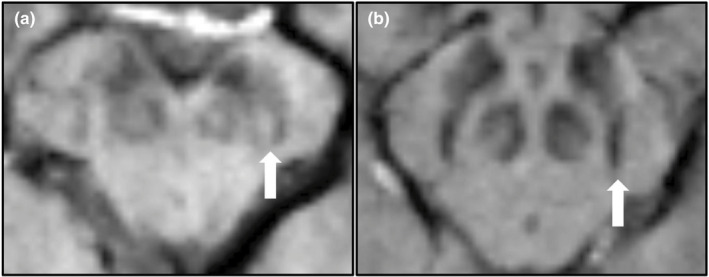
\includegraphics[width=0.8\linewidth]{FileAusiliari/Immagini/degenerative/BRB3-11-e02202-g002}
	\caption{Esempi di segno della coda di rondine (STS) in un individuo malato (a) e di STS assente in un individuo sano (b). Sono mostrate sezioni assiali del mesencefalo mappate tramite imaging pesato con suscettibilità (SWI). Le frecce bianche indicano la diversa configurazione del Nigrosoma-1 (N1). Da Brain Behav. 2021 May 24;11(7):e02202. doi: 10.1002/brb3.2202}
	\label{fig:brb3-11-e02202-g002}
\end{figure*}


La diagnosi differenziale delle sindromi parkinsoniane atipiche beneficia significativamente dell'imaging RM. L'atrofia multisistemica (MSA) evidenzia caratteristica atrofia putaminale, pontica e cerebellare, con ipointensità putaminale T2/SWI e "hot cross bun sign" pontino. La paralisi sopranucleare progressiva (PSP) manifesta atrofia mesencefalica con alterazione del rapporto mesencefalo-ponte, mentre la degenerazione corticobasale (CBD) presenta atrofia frontoparietale asimmetrica con iperintensità della sostanza bianca subcorticale.
Metodiche avanzate quali Diffusion Tensor Imaging (DTI) e risonanza magnetica funzionale (fMRI) consentono la caratterizzazione delle alterazioni microstrutturali della sostanza bianca e delle modificazioni funzionali cerebrali, sebbene la sensibilità nell'identificazione della progressione patologica e nella valutazione della risposta terapeutica necessiti ulteriore validazione. Le limitazioni metodologiche includono variabilità interindividuale e sovrapposizione dei reperti radiologici nelle diverse sindromi parkinsoniane.

\subsection{Trattamento e prognosi}

\subsection{Checklist di refertazione}

\begin{itemize}[label=$\square$] % Riquadro vuoto come simbolo
	\item Escludi altre cause di parkinsonismo (es ictus)
	\item Controlla il segnale dei nigrosomi
	\item Controlla il trofismo delle strutture sottotentoriali
\end{itemize}

\subsection{Bibliografia}
\small{
	
	
}

\note{Nota a margine}
\expl{Nota a margine colorata}
\input{Capitoli/degenerative/approccio.tex}
\input{Capitoli/degenerative/degenerative.tex}
\section{Morbo di Parkinson}

\subsection{Definizione}

\subsection{Eziologia}

\begin{figure*}[h]
	\centering
	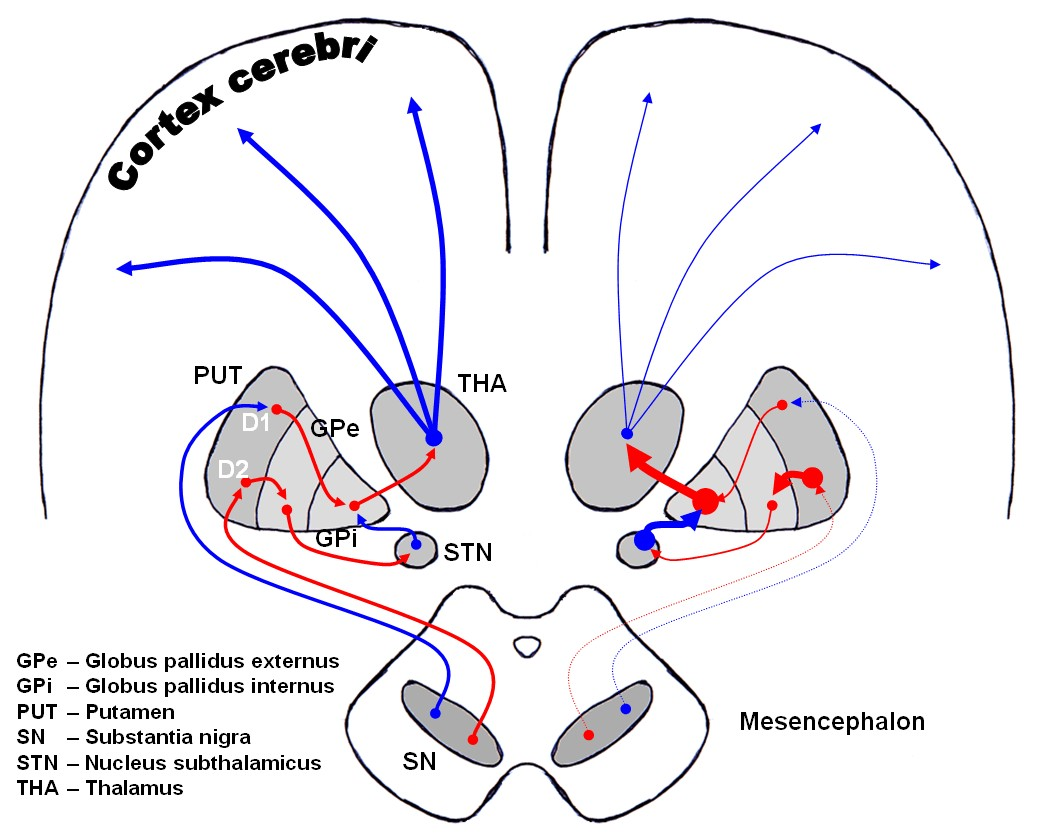
\includegraphics[width=0.5\linewidth]{FileAusiliari/Immagini/degenerative/dopamine-in-parkinsons-disease-illustration}
	\caption[Vie dopaminergiche]{L'immagine mostra le vie dopaminergiche del cervello umano in condizioni normali (a sinistra) e nella malattia di Parkinson (a destra). Le frecce rosse indicano la soppressione del bersaglio, quelle blu la stimolazione della struttura bersaglio. Caso per gentile concessione di Wikipedia, Radiopaedia.org, rID: 36286}
	\label{fig:dopamine-in-parkinsons-disease-illustration}
\end{figure*}

\subsection{Epidemiologia}
Il MP costituisce una delle principali cause di disabilità e mortalità nell'ambito delle patologie neurologiche, con una prevalenza particolarmente elevata negli Stati Uniti e in Canada (160-180 casi/100.000 abitanti). L'incidenza annuale in Nord America oscilla tra 108 e 212 casi ogni 100.000 individui di età $\geq$65 anni, con una prevalenza dello 0,3\% nella popolazione adulta $\geq$40 anni e dell'1,6\% nei soggetti ultrasessantacinquenni.
L'esordio della patologia mostra una significativa correlazione con l'età, manifestandosi tipicamente dalla quinta decade di vita, con un'età media alla diagnosi di 70,5 anni e una finestra di esordio prevalente tra i 45 e i 70 anni. Una variante giovanile può presentarsi tra i 20 e i 40 anni, sebbene l'esordio prima dei 30 anni risulti infrequente. La distribuzione per sesso evidenzia una predominanza maschile, particolarmente accentuata nella fascia d'età 50-60 anni.
L'eziologia del MP comprende fattori di rischio genetici, con particolare rilevanza nelle forme ad esordio precoce, e ambientali, tra cui l'esposizione a pesticidi e inquinanti atmosferici. Sono stati identificati fattori protettivi, inclusi il consumo di caffè, l'attività fisica e il fumo di sigaretta. La patologia si presenta prevalentemente in forma sporadica (85-90\% dei casi), mentre una minoranza dei casi (10-15\%) presenta familiarità positiva.

\subsubsection{Fattori di rischio}
L'eziopatogenesi del Morbo di Parkinson (MP) presenta una complessa interazione di fattori di rischio genetici, ambientali e non modificabili. L'anamnesi familiare positiva per MP in consanguinei di primo grado comporta un incremento del rischio relativo di 2-3 volte. Le forme monogeniche, rappresentanti meno del 10\% della casistica totale, manifestano pattern di ereditarietà autosomica dominante, recessiva o X-linked, caratterizzandosi per un esordio precoce rispetto alle forme sporadiche.
Le mutazioni eterozigoti del gene GBA1 costituiscono un significativo fattore di rischio genetico, unitamente ad alterazioni di altri geni codificanti per enzimi lisosomiali. Il coinvolgimento di geni quali SNCA, LRRK2, VPS35, Parkin, PINK1 e DJ-1 è stato ampiamente documentato. Particolare rilevanza assumono le mutazioni del gene Nurr1, determinante per l'identità neuronale dopaminergica, e del gene DJ-1, cruciale nella risposta allo stress ossidativo. Le alterazioni del gene PINK1, codificante per una chinasi mitocondriale, e del gene Park2, responsabile della sintesi della proteina parkina, sono associate a forme ad esordio precoce.
L'esposizione a neurotossine ambientali, inclusi mercurio, manganese, disolfuro di carbonio, solventi organici, MPTP e monossido di carbonio, può indurre degenerazione nigrostriatale e parkinsonismo. L'uso di neurolettici e l'abuso endovenoso di efedrone possono causare sindromi parkinsoniane potenzialmente irreversibili. Traumi cranici ripetuti, pesticidi, solventi e inquinamento atmosferico rappresentano ulteriori fattori di rischio ambientale documentati.
Tra i fattori non modificabili, l'età avanzata e il sesso maschile emergono come significativi predittori di rischio, con predominanza nella sesta decade di vita. Comorbidità quali depressione, ansia, stipsi, diabete mellito tipo 2, obesità e alterazioni del metabolismo del ferro sono state correlate a un incrementato rischio di MP.
Il consumo di tabacco e caffè, unitamente all'attività fisica regolare, ha mostrato effetti protettivi, sebbene di modesta entità. È fondamentale sottolineare che la maggioranza dei casi di MP rimane idiopatica, suggerendo un'eziologia multifattoriale.

\subsection{Presentazione  clinica}
La sintomatologia del Morbo di Parkinson manifesta un quadro clinico caratterizzato da manifestazioni motorie cardinali e sintomatologia non motoria associata. Il complesso sintomatologico motorio comprende tremore a riposo spesso asimmetrico con frequenza di 4-6 Hz, tipicamente descritto come "pill-rolling", bradicinesia manifestantesi con rallentamento motorio, ipomimia e ridotta oscillazione pendolare degli arti superiori durante la deambulazione, rigidità muscolare ("lead-pipe" o fenomeno della ruota dentata), e instabilità posturale documentabile attraverso il test della retropulsione. La deambulazione risulta caratterizzata da una progressione a piccoli passi con tendenza allo strascicamento e ridotta oscillazione degli arti superiori.
La sintomatologia accessoria include disartria con eloquio esplosivo secondario a incoordinazione linguo-diaframmatica, movimenti involontari della lingua con conseguente difficoltà protrusiva, e incremento della frequenza di ammiccamento palpebrale, quest'ultimo in contrasto con quanto osservato nella corea di Huntington. La disfunzione autonomica, i disturbi olfattivi, la sintomatologia algica, le alterazioni sensitive e i disturbi timici costituiscono il corredo sintomatologico non motorio. Il deterioramento cognitivo, con particolare coinvolgimento delle funzioni attentive, può manifestarsi e progredire nel decorso della patologia.
La progressione temporale della malattia evidenzia un esordio tipicamente unilaterale con successiva bilateralizzazione, manifestandosi prevalentemente nella sesta decade di vita. La responsività alla terapia dopaminergica, in particolare alla levodopa, rappresenta un elemento caratteristico, sebbene il tremore possa risultare farmacoresistente, in contrasto con la significativa risposta della bradicinesia e della rigidità. La variabilità fenotipica interindividuale costituisce un elemento distintivo della patologia.

\subsection{Approccio diagnostico}
L'iter diagnostico della malattia di Parkinson si fonda primariamente sulla valutazione clinica, data l'assenza di biomarcatori patognomonici. La diagnosi richiede la documentazione di bradicinesia associata ad almeno un sintomo cardine tra tremore a riposo o rigidità, valutati mediante la scala MDS-UPDRS standardizzata.
L'approccio diagnostico contempla un'accurata anamnesi ed esame obiettivo neurologico, focalizzati sull'identificazione dei sintomi cardinali: bradicinesia, tremore a riposo (4-6 Hz) tipicamente asimmetrico, rigidità e instabilità posturale. La responsività alla terapia dopaminergica, particolarmente evidente per bradicinesia e rigidità, costituisce un elemento diagnostico supportivo significativo, mentre una mancata risposta a dosaggi adeguati di levodopa suggerisce diagnosi alternative.
L'esclusione di parkinsonismi secondari richiede particolare attenzione all'insorgenza temporale dei sintomi e alla distribuzione topografica del coinvolgimento motorio. La diagnostica per immagini, sebbene non necessaria nelle presentazioni cliniche tipiche con adeguata risposta alla levodopa, può includere RM cerebrale, particolarmente utile mediante sequenze SWI per la valutazione del "swallow tail sign" nigrostriatale. La SPECT con 123I-FP-CIT (DaTscan) documenta la disfunzione dopaminergica presinaptica, mentre la PET con FDG consente la differenziazione metabolica tra PD e sindromi parkinsoniane atipiche.
L'analisi genetica, indicata in casi selezionati (esordio precoce, familiarità positiva, specifiche etnie), e la valutazione autonomica mediante scintigrafia miocardica con MIBG, che evidenzia la denervazione simpatica caratteristica, completano l'iter diagnostico. L'ecografia transcranica può evidenziare l'iperecogenicità della sostanza nera, supportando la diagnosi differenziale.
I criteri MDS stratificano la diagnosi in PD clinicamente stabilita e probabile, bilanciando specificità e sensibilità diagnostica nella pratica clinica.

\begin{Oss}
	La scala MDS-UPDRS (Movement Disorder Society-Unified Parkinson's Disease Rating Scale) è uno strumento di valutazione clinica ampiamente utilizzato per quantificare la gravità dei sintomi motori e non motori della malattia di Parkinson. Questa scala è stata sviluppata per migliorare la consistenza nella valutazione dei sintomi e per integrare meglio gli aspetti non motori della PD.
	Struttura: La scala MDS-UPDRS è composta da quattro sezioni:
	\begin{description}
		\item[Sezione I]{Esperienze non motorie della vita quotidiana. Questa sezione valuta aspetti come le capacità cognitive, i disturbi comportamentali e dell'umore}
		\item [Sezione II]{Esperienze motorie della vita quotidiana. Questa sezione valuta l'impatto dei sintomi motori sulle attività quotidiane}
		\item [Sezione III]{Esame motorio. Questa sezione valuta i segni motori della PD attraverso un esame clinico, come il tremore, la rigidità e la bradicinesia}
		\item[Sezione IV]{Complicanze della terapia. Questa sezione valuta le complicanze associate al trattamento farmacologico}
	\end{description}
	Il punteggio totale per le sezioni I-IV varia da 0 (nessuna disabilità) a 199 (disabilità totale). La sezione III, che valuta i sintomi motori, ha un punteggio che varia da 0 a 132.
	Oltre alla scala MDS-UPDRS, esistono altre scale di valutazione utilizzate nella PD, come la scala di Hoehn e Yahr e la scala di Schwab e England. La scala di Hoehn e Yahr valuta la gravità della malattia da 0 (nessuna malattia) a 5 (paziente costretto su sedia a rotelle o allettato senza assistenza).
\end{Oss}

\subsection{Anatomia patologica}
Dal punto di vista anatomopatologico il morbo di Parkinson si manifesta attraverso inclusioni proteiche intraneuronali denominate corpi di Lewy, costituiti primariamente da aggregati patologici di alfa-sinucleina, una proteina sinaptica fisiologicamente presente nel sistema nervoso centrale. L'accumulo di queste inclusioni, sebbene non patognomonico del morbo di Parkinson essendo documentabile anche nella demenza a corpi di Lewy, rappresenta una caratteristica istopatologica fondamentale quando localizzato nella substantia nigra, in associazione alla perdita neuronale dopaminergica. L'assenza di corpi di Lewy nelle forme post-encefalitiche, caratterizzate invece da grovigli neurofibrillari, e in alcune forme geneticamente determinate, sottolinea l'eterogeneità patogenetica della malattia.
La progressione spazio-temporale della patologia, codificata nello staging di Braak, delinea sei stadi evolutivi caratterizzati da una diffusione ascendente delle alterazioni neuropatologiche. Gli stadi iniziali (1-2) coinvolgono il nucleo motore dorsale dei nervi glossofaringeo e vago e il nucleo olfattivo anteriore, precedendo frequentemente la sintomatologia motoria. Gli stadi intermedi (3-4) documentano il coinvolgimento della substantia nigra pars compacta, del prosencefalo basale e della mesocorteccia temporale, correlando con l'esordio clinico della malattia. Gli stadi terminali (5-6) evidenziano una progressione neocorticale diffusa.
La patogenesi molecolare implica alterazioni del metabolismo dell'alfa-sinucleina, potenzialmente accelerate da disfunzioni delle proteine heat shock o dall'azione della dopamina. Il coinvolgimento della proteina parkin nella degradazione proteasomica evidenzia meccanismi neurodegenerativi potenzialmente indipendenti dalla formazione dei corpi di Lewy.
L'alfa-sinucleina, proteina fisiologicamente localizzata nelle terminazioni presinaptiche neuronali, manifesta nella patogenesi del morbo di Parkinson un processo patologico caratterizzato da misfolding proteico e successiva aggregazione in oligomeri, protofibrille e fibrille, culminante nella formazione dei corpi di Lewy intraneuronali. Questi aggregati proteici, considerati hallmark istopatologico della malattia, evidenziano particolare neurotossicità nella forma protofibrillare, determinando disfunzione e successiva degenerazione neuronale dopaminergica nigrostriatale.
L'identificazione di mutazioni nel gene SNCA, codificante per l'alfa-sinucleina, nelle forme familiari di malattia, unitamente alla documentazione di fenotipi clinici particolarmente aggressivi in presenza di duplicazione o triplicazione genica, ha fornito evidenze significative del ruolo causale di questa proteina nella patogenesi della malattia. La documentata capacità di trasmissione transcellulare dell'alfa-sinucleina patologica costituisce il substrato molecolare della progressione anatomopatologica descritta nello staging di Braak.
La disfunzione sinaptica correlata all'accumulo di alfa-sinucleina rappresenta un meccanismo patogenetico critico, modulato da fattori quali stress ossidativo, alterazioni del sistema ubiquitina-proteasoma e interazione con il metabolismo dopaminergico. Mutazioni nei geni parkin, PINK1 e DJ-1 influenzano il metabolismo dell'alfa-sinucleina attraverso alterazioni dei sistemi di degradazione proteica.
L'alfa-sinucleina costituisce attualmente un promettente target terapeutico, con particolare interesse per lo sviluppo di anticorpi monoclonali specifici e inibitori dell'aggregazione proteica, finalizzati al rallentamento della progressione patologica.

\subsection{Imaging}

\subsubsection{TC}
La TC manifesta un'utilità clinica circoscritta nella valutazione diagnostica primaria del MP, assumendo rilevanza nell'esclusione di patologie strutturali mimiche quali lesioni espansive, idrocefalo o alterazioni vascolari, particolarmente in presenza di presentazioni cliniche atipiche o "red flags" suggestive di diagnosi alternative.
Nel contesto della gestione terapeutica, la TC assume particolare rilevanza nella valutazione post-chirurgica della stimolazione cerebrale profonda (DBS), consentendo la verifica del corretto posizionamento degli elettrodi nel nucleo subtalamico (STN), tipicamente localizzati a 9mm dalla linea mediana, e l'identificazione di eventuali complicanze post-procedurali quali eventi emorragici, ischemici o fenomeni infiammatori transitori, questi ultimi caratterizzati da aree ipodense perilettrodiche a risoluzione graduale. L'utilità della metodica nel follow-up routinario post-DBS risulta secondaria.
La sensibilità subottimale della TC nella diagnosi differenziale tra PD e sindromi parkinsoniane atipiche, incluse atrofia multisistemica e paralisi sopranucleare progressiva, nonché nella distinzione dal tremore essenziale, ne limita significativamente l'applicazione clinica in questo contesto diagnostico.

\subsubsection{RM}
La RM è frequentemente normale nelle sequenze convenzionali (T1, T2, FLAIR) nelle fasi iniziali di malattia. L'implementazione di sequenze susceptibility-weighted imaging (SWI) o T2*-weighted ad alta risoluzione consente la visualizzazione del nigrosoma-1, struttura caratterizzata dal patognomonico "swallow tail sign", la cui perdita correla con la degenerazione dopaminergica nigrostriatale. L'accumulo patologico di ferro nella substantia nigra, quantificabile mediante sequenze SWI/T2* e incrementato del 50\% rispetto ai controlli, costituisce un ulteriore marker diagnostico, complementato dall'imaging della neuromelanina mediante sequenze T1 con impulsi di trasferimento di magnetizzazione (MTC).

\begin{figure*}[h]
	\centering
	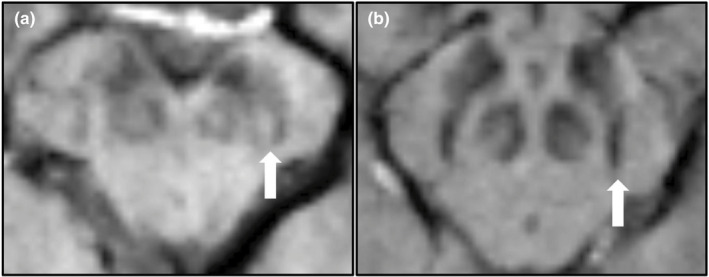
\includegraphics[width=0.8\linewidth]{FileAusiliari/Immagini/degenerative/BRB3-11-e02202-g002}
	\caption{Esempi di segno della coda di rondine (STS) in un individuo malato (a) e di STS assente in un individuo sano (b). Sono mostrate sezioni assiali del mesencefalo mappate tramite imaging pesato con suscettibilità (SWI). Le frecce bianche indicano la diversa configurazione del Nigrosoma-1 (N1). Da Brain Behav. 2021 May 24;11(7):e02202. doi: 10.1002/brb3.2202}
	\label{fig:brb3-11-e02202-g002}
\end{figure*}


La diagnosi differenziale delle sindromi parkinsoniane atipiche beneficia significativamente dell'imaging RM. L'atrofia multisistemica (MSA) evidenzia caratteristica atrofia putaminale, pontica e cerebellare, con ipointensità putaminale T2/SWI e "hot cross bun sign" pontino. La paralisi sopranucleare progressiva (PSP) manifesta atrofia mesencefalica con alterazione del rapporto mesencefalo-ponte, mentre la degenerazione corticobasale (CBD) presenta atrofia frontoparietale asimmetrica con iperintensità della sostanza bianca subcorticale.
Metodiche avanzate quali Diffusion Tensor Imaging (DTI) e risonanza magnetica funzionale (fMRI) consentono la caratterizzazione delle alterazioni microstrutturali della sostanza bianca e delle modificazioni funzionali cerebrali, sebbene la sensibilità nell'identificazione della progressione patologica e nella valutazione della risposta terapeutica necessiti ulteriore validazione. Le limitazioni metodologiche includono variabilità interindividuale e sovrapposizione dei reperti radiologici nelle diverse sindromi parkinsoniane.

\subsection{Trattamento e prognosi}

\subsection{Checklist di refertazione}

\begin{itemize}[label=$\square$] % Riquadro vuoto come simbolo
	\item Escludi altre cause di parkinsonismo (es ictus)
	\item Controlla il segnale dei nigrosomi
	\item Controlla il trofismo delle strutture sottotentoriali
\end{itemize}

\subsection{Bibliografia}
\small{
	
	
}

\note{Nota a margine}
\expl{Nota a margine colorata}
\input{Capitoli/degenerative/approccio.tex}
\input{Capitoli/degenerative/degenerative.tex}
\section{Morbo di Parkinson}

\subsection{Definizione}

\subsection{Eziologia}

\begin{figure*}[h]
	\centering
	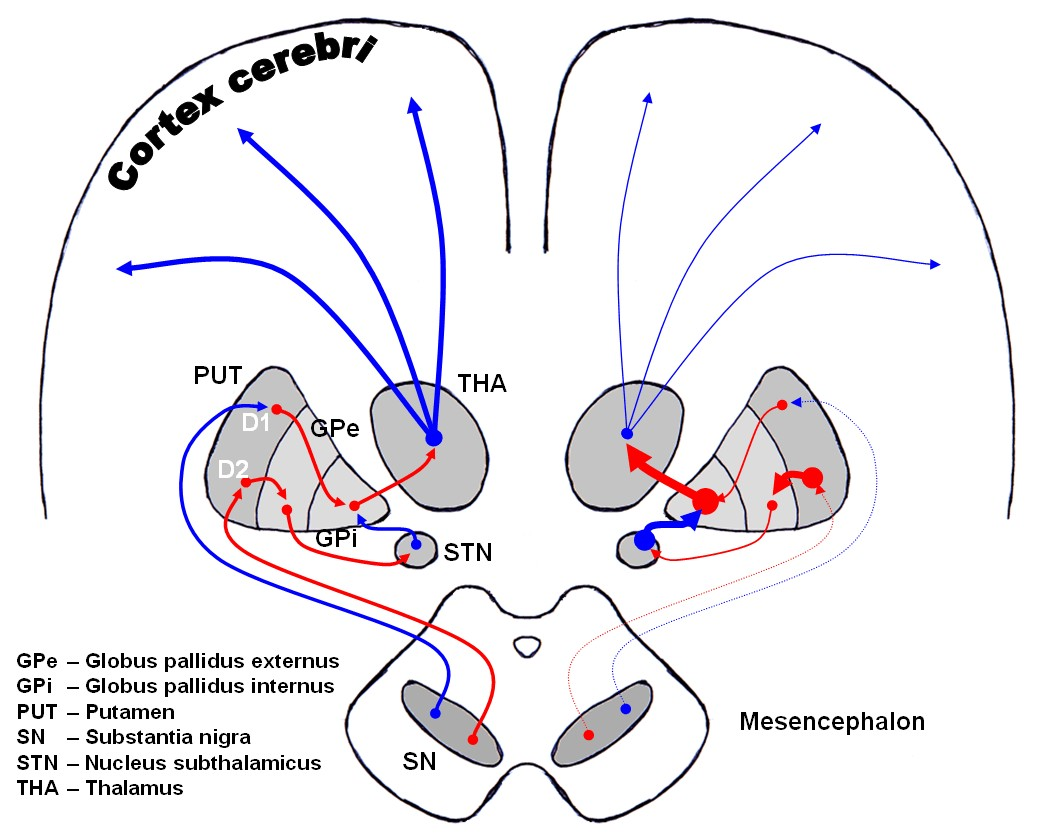
\includegraphics[width=0.5\linewidth]{FileAusiliari/Immagini/degenerative/dopamine-in-parkinsons-disease-illustration}
	\caption[Vie dopaminergiche]{L'immagine mostra le vie dopaminergiche del cervello umano in condizioni normali (a sinistra) e nella malattia di Parkinson (a destra). Le frecce rosse indicano la soppressione del bersaglio, quelle blu la stimolazione della struttura bersaglio. Caso per gentile concessione di Wikipedia, Radiopaedia.org, rID: 36286}
	\label{fig:dopamine-in-parkinsons-disease-illustration}
\end{figure*}

\subsection{Epidemiologia}
Il MP costituisce una delle principali cause di disabilità e mortalità nell'ambito delle patologie neurologiche, con una prevalenza particolarmente elevata negli Stati Uniti e in Canada (160-180 casi/100.000 abitanti). L'incidenza annuale in Nord America oscilla tra 108 e 212 casi ogni 100.000 individui di età $\geq$65 anni, con una prevalenza dello 0,3\% nella popolazione adulta $\geq$40 anni e dell'1,6\% nei soggetti ultrasessantacinquenni.
L'esordio della patologia mostra una significativa correlazione con l'età, manifestandosi tipicamente dalla quinta decade di vita, con un'età media alla diagnosi di 70,5 anni e una finestra di esordio prevalente tra i 45 e i 70 anni. Una variante giovanile può presentarsi tra i 20 e i 40 anni, sebbene l'esordio prima dei 30 anni risulti infrequente. La distribuzione per sesso evidenzia una predominanza maschile, particolarmente accentuata nella fascia d'età 50-60 anni.
L'eziologia del MP comprende fattori di rischio genetici, con particolare rilevanza nelle forme ad esordio precoce, e ambientali, tra cui l'esposizione a pesticidi e inquinanti atmosferici. Sono stati identificati fattori protettivi, inclusi il consumo di caffè, l'attività fisica e il fumo di sigaretta. La patologia si presenta prevalentemente in forma sporadica (85-90\% dei casi), mentre una minoranza dei casi (10-15\%) presenta familiarità positiva.

\subsubsection{Fattori di rischio}
L'eziopatogenesi del Morbo di Parkinson (MP) presenta una complessa interazione di fattori di rischio genetici, ambientali e non modificabili. L'anamnesi familiare positiva per MP in consanguinei di primo grado comporta un incremento del rischio relativo di 2-3 volte. Le forme monogeniche, rappresentanti meno del 10\% della casistica totale, manifestano pattern di ereditarietà autosomica dominante, recessiva o X-linked, caratterizzandosi per un esordio precoce rispetto alle forme sporadiche.
Le mutazioni eterozigoti del gene GBA1 costituiscono un significativo fattore di rischio genetico, unitamente ad alterazioni di altri geni codificanti per enzimi lisosomiali. Il coinvolgimento di geni quali SNCA, LRRK2, VPS35, Parkin, PINK1 e DJ-1 è stato ampiamente documentato. Particolare rilevanza assumono le mutazioni del gene Nurr1, determinante per l'identità neuronale dopaminergica, e del gene DJ-1, cruciale nella risposta allo stress ossidativo. Le alterazioni del gene PINK1, codificante per una chinasi mitocondriale, e del gene Park2, responsabile della sintesi della proteina parkina, sono associate a forme ad esordio precoce.
L'esposizione a neurotossine ambientali, inclusi mercurio, manganese, disolfuro di carbonio, solventi organici, MPTP e monossido di carbonio, può indurre degenerazione nigrostriatale e parkinsonismo. L'uso di neurolettici e l'abuso endovenoso di efedrone possono causare sindromi parkinsoniane potenzialmente irreversibili. Traumi cranici ripetuti, pesticidi, solventi e inquinamento atmosferico rappresentano ulteriori fattori di rischio ambientale documentati.
Tra i fattori non modificabili, l'età avanzata e il sesso maschile emergono come significativi predittori di rischio, con predominanza nella sesta decade di vita. Comorbidità quali depressione, ansia, stipsi, diabete mellito tipo 2, obesità e alterazioni del metabolismo del ferro sono state correlate a un incrementato rischio di MP.
Il consumo di tabacco e caffè, unitamente all'attività fisica regolare, ha mostrato effetti protettivi, sebbene di modesta entità. È fondamentale sottolineare che la maggioranza dei casi di MP rimane idiopatica, suggerendo un'eziologia multifattoriale.

\subsection{Presentazione  clinica}
La sintomatologia del Morbo di Parkinson manifesta un quadro clinico caratterizzato da manifestazioni motorie cardinali e sintomatologia non motoria associata. Il complesso sintomatologico motorio comprende tremore a riposo spesso asimmetrico con frequenza di 4-6 Hz, tipicamente descritto come "pill-rolling", bradicinesia manifestantesi con rallentamento motorio, ipomimia e ridotta oscillazione pendolare degli arti superiori durante la deambulazione, rigidità muscolare ("lead-pipe" o fenomeno della ruota dentata), e instabilità posturale documentabile attraverso il test della retropulsione. La deambulazione risulta caratterizzata da una progressione a piccoli passi con tendenza allo strascicamento e ridotta oscillazione degli arti superiori.
La sintomatologia accessoria include disartria con eloquio esplosivo secondario a incoordinazione linguo-diaframmatica, movimenti involontari della lingua con conseguente difficoltà protrusiva, e incremento della frequenza di ammiccamento palpebrale, quest'ultimo in contrasto con quanto osservato nella corea di Huntington. La disfunzione autonomica, i disturbi olfattivi, la sintomatologia algica, le alterazioni sensitive e i disturbi timici costituiscono il corredo sintomatologico non motorio. Il deterioramento cognitivo, con particolare coinvolgimento delle funzioni attentive, può manifestarsi e progredire nel decorso della patologia.
La progressione temporale della malattia evidenzia un esordio tipicamente unilaterale con successiva bilateralizzazione, manifestandosi prevalentemente nella sesta decade di vita. La responsività alla terapia dopaminergica, in particolare alla levodopa, rappresenta un elemento caratteristico, sebbene il tremore possa risultare farmacoresistente, in contrasto con la significativa risposta della bradicinesia e della rigidità. La variabilità fenotipica interindividuale costituisce un elemento distintivo della patologia.

\subsection{Approccio diagnostico}
L'iter diagnostico della malattia di Parkinson si fonda primariamente sulla valutazione clinica, data l'assenza di biomarcatori patognomonici. La diagnosi richiede la documentazione di bradicinesia associata ad almeno un sintomo cardine tra tremore a riposo o rigidità, valutati mediante la scala MDS-UPDRS standardizzata.
L'approccio diagnostico contempla un'accurata anamnesi ed esame obiettivo neurologico, focalizzati sull'identificazione dei sintomi cardinali: bradicinesia, tremore a riposo (4-6 Hz) tipicamente asimmetrico, rigidità e instabilità posturale. La responsività alla terapia dopaminergica, particolarmente evidente per bradicinesia e rigidità, costituisce un elemento diagnostico supportivo significativo, mentre una mancata risposta a dosaggi adeguati di levodopa suggerisce diagnosi alternative.
L'esclusione di parkinsonismi secondari richiede particolare attenzione all'insorgenza temporale dei sintomi e alla distribuzione topografica del coinvolgimento motorio. La diagnostica per immagini, sebbene non necessaria nelle presentazioni cliniche tipiche con adeguata risposta alla levodopa, può includere RM cerebrale, particolarmente utile mediante sequenze SWI per la valutazione del "swallow tail sign" nigrostriatale. La SPECT con 123I-FP-CIT (DaTscan) documenta la disfunzione dopaminergica presinaptica, mentre la PET con FDG consente la differenziazione metabolica tra PD e sindromi parkinsoniane atipiche.
L'analisi genetica, indicata in casi selezionati (esordio precoce, familiarità positiva, specifiche etnie), e la valutazione autonomica mediante scintigrafia miocardica con MIBG, che evidenzia la denervazione simpatica caratteristica, completano l'iter diagnostico. L'ecografia transcranica può evidenziare l'iperecogenicità della sostanza nera, supportando la diagnosi differenziale.
I criteri MDS stratificano la diagnosi in PD clinicamente stabilita e probabile, bilanciando specificità e sensibilità diagnostica nella pratica clinica.

\begin{Oss}
	La scala MDS-UPDRS (Movement Disorder Society-Unified Parkinson's Disease Rating Scale) è uno strumento di valutazione clinica ampiamente utilizzato per quantificare la gravità dei sintomi motori e non motori della malattia di Parkinson. Questa scala è stata sviluppata per migliorare la consistenza nella valutazione dei sintomi e per integrare meglio gli aspetti non motori della PD.
	Struttura: La scala MDS-UPDRS è composta da quattro sezioni:
	\begin{description}
		\item[Sezione I]{Esperienze non motorie della vita quotidiana. Questa sezione valuta aspetti come le capacità cognitive, i disturbi comportamentali e dell'umore}
		\item [Sezione II]{Esperienze motorie della vita quotidiana. Questa sezione valuta l'impatto dei sintomi motori sulle attività quotidiane}
		\item [Sezione III]{Esame motorio. Questa sezione valuta i segni motori della PD attraverso un esame clinico, come il tremore, la rigidità e la bradicinesia}
		\item[Sezione IV]{Complicanze della terapia. Questa sezione valuta le complicanze associate al trattamento farmacologico}
	\end{description}
	Il punteggio totale per le sezioni I-IV varia da 0 (nessuna disabilità) a 199 (disabilità totale). La sezione III, che valuta i sintomi motori, ha un punteggio che varia da 0 a 132.
	Oltre alla scala MDS-UPDRS, esistono altre scale di valutazione utilizzate nella PD, come la scala di Hoehn e Yahr e la scala di Schwab e England. La scala di Hoehn e Yahr valuta la gravità della malattia da 0 (nessuna malattia) a 5 (paziente costretto su sedia a rotelle o allettato senza assistenza).
\end{Oss}

\subsection{Anatomia patologica}
Dal punto di vista anatomopatologico il morbo di Parkinson si manifesta attraverso inclusioni proteiche intraneuronali denominate corpi di Lewy, costituiti primariamente da aggregati patologici di alfa-sinucleina, una proteina sinaptica fisiologicamente presente nel sistema nervoso centrale. L'accumulo di queste inclusioni, sebbene non patognomonico del morbo di Parkinson essendo documentabile anche nella demenza a corpi di Lewy, rappresenta una caratteristica istopatologica fondamentale quando localizzato nella substantia nigra, in associazione alla perdita neuronale dopaminergica. L'assenza di corpi di Lewy nelle forme post-encefalitiche, caratterizzate invece da grovigli neurofibrillari, e in alcune forme geneticamente determinate, sottolinea l'eterogeneità patogenetica della malattia.
La progressione spazio-temporale della patologia, codificata nello staging di Braak, delinea sei stadi evolutivi caratterizzati da una diffusione ascendente delle alterazioni neuropatologiche. Gli stadi iniziali (1-2) coinvolgono il nucleo motore dorsale dei nervi glossofaringeo e vago e il nucleo olfattivo anteriore, precedendo frequentemente la sintomatologia motoria. Gli stadi intermedi (3-4) documentano il coinvolgimento della substantia nigra pars compacta, del prosencefalo basale e della mesocorteccia temporale, correlando con l'esordio clinico della malattia. Gli stadi terminali (5-6) evidenziano una progressione neocorticale diffusa.
La patogenesi molecolare implica alterazioni del metabolismo dell'alfa-sinucleina, potenzialmente accelerate da disfunzioni delle proteine heat shock o dall'azione della dopamina. Il coinvolgimento della proteina parkin nella degradazione proteasomica evidenzia meccanismi neurodegenerativi potenzialmente indipendenti dalla formazione dei corpi di Lewy.
L'alfa-sinucleina, proteina fisiologicamente localizzata nelle terminazioni presinaptiche neuronali, manifesta nella patogenesi del morbo di Parkinson un processo patologico caratterizzato da misfolding proteico e successiva aggregazione in oligomeri, protofibrille e fibrille, culminante nella formazione dei corpi di Lewy intraneuronali. Questi aggregati proteici, considerati hallmark istopatologico della malattia, evidenziano particolare neurotossicità nella forma protofibrillare, determinando disfunzione e successiva degenerazione neuronale dopaminergica nigrostriatale.
L'identificazione di mutazioni nel gene SNCA, codificante per l'alfa-sinucleina, nelle forme familiari di malattia, unitamente alla documentazione di fenotipi clinici particolarmente aggressivi in presenza di duplicazione o triplicazione genica, ha fornito evidenze significative del ruolo causale di questa proteina nella patogenesi della malattia. La documentata capacità di trasmissione transcellulare dell'alfa-sinucleina patologica costituisce il substrato molecolare della progressione anatomopatologica descritta nello staging di Braak.
La disfunzione sinaptica correlata all'accumulo di alfa-sinucleina rappresenta un meccanismo patogenetico critico, modulato da fattori quali stress ossidativo, alterazioni del sistema ubiquitina-proteasoma e interazione con il metabolismo dopaminergico. Mutazioni nei geni parkin, PINK1 e DJ-1 influenzano il metabolismo dell'alfa-sinucleina attraverso alterazioni dei sistemi di degradazione proteica.
L'alfa-sinucleina costituisce attualmente un promettente target terapeutico, con particolare interesse per lo sviluppo di anticorpi monoclonali specifici e inibitori dell'aggregazione proteica, finalizzati al rallentamento della progressione patologica.

\subsection{Imaging}

\subsubsection{TC}
La TC manifesta un'utilità clinica circoscritta nella valutazione diagnostica primaria del MP, assumendo rilevanza nell'esclusione di patologie strutturali mimiche quali lesioni espansive, idrocefalo o alterazioni vascolari, particolarmente in presenza di presentazioni cliniche atipiche o "red flags" suggestive di diagnosi alternative.
Nel contesto della gestione terapeutica, la TC assume particolare rilevanza nella valutazione post-chirurgica della stimolazione cerebrale profonda (DBS), consentendo la verifica del corretto posizionamento degli elettrodi nel nucleo subtalamico (STN), tipicamente localizzati a 9mm dalla linea mediana, e l'identificazione di eventuali complicanze post-procedurali quali eventi emorragici, ischemici o fenomeni infiammatori transitori, questi ultimi caratterizzati da aree ipodense perilettrodiche a risoluzione graduale. L'utilità della metodica nel follow-up routinario post-DBS risulta secondaria.
La sensibilità subottimale della TC nella diagnosi differenziale tra PD e sindromi parkinsoniane atipiche, incluse atrofia multisistemica e paralisi sopranucleare progressiva, nonché nella distinzione dal tremore essenziale, ne limita significativamente l'applicazione clinica in questo contesto diagnostico.

\subsubsection{RM}
La RM è frequentemente normale nelle sequenze convenzionali (T1, T2, FLAIR) nelle fasi iniziali di malattia. L'implementazione di sequenze susceptibility-weighted imaging (SWI) o T2*-weighted ad alta risoluzione consente la visualizzazione del nigrosoma-1, struttura caratterizzata dal patognomonico "swallow tail sign", la cui perdita correla con la degenerazione dopaminergica nigrostriatale. L'accumulo patologico di ferro nella substantia nigra, quantificabile mediante sequenze SWI/T2* e incrementato del 50\% rispetto ai controlli, costituisce un ulteriore marker diagnostico, complementato dall'imaging della neuromelanina mediante sequenze T1 con impulsi di trasferimento di magnetizzazione (MTC).

\begin{figure*}[h]
	\centering
	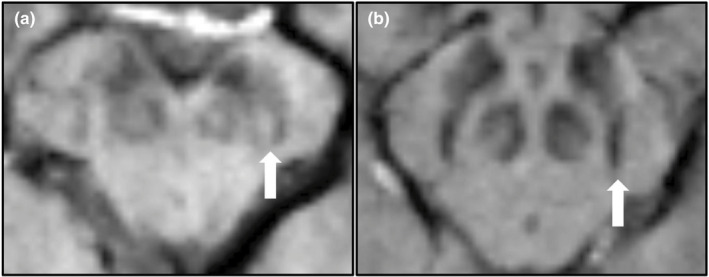
\includegraphics[width=0.8\linewidth]{FileAusiliari/Immagini/degenerative/BRB3-11-e02202-g002}
	\caption{Esempi di segno della coda di rondine (STS) in un individuo malato (a) e di STS assente in un individuo sano (b). Sono mostrate sezioni assiali del mesencefalo mappate tramite imaging pesato con suscettibilità (SWI). Le frecce bianche indicano la diversa configurazione del Nigrosoma-1 (N1). Da Brain Behav. 2021 May 24;11(7):e02202. doi: 10.1002/brb3.2202}
	\label{fig:brb3-11-e02202-g002}
\end{figure*}


La diagnosi differenziale delle sindromi parkinsoniane atipiche beneficia significativamente dell'imaging RM. L'atrofia multisistemica (MSA) evidenzia caratteristica atrofia putaminale, pontica e cerebellare, con ipointensità putaminale T2/SWI e "hot cross bun sign" pontino. La paralisi sopranucleare progressiva (PSP) manifesta atrofia mesencefalica con alterazione del rapporto mesencefalo-ponte, mentre la degenerazione corticobasale (CBD) presenta atrofia frontoparietale asimmetrica con iperintensità della sostanza bianca subcorticale.
Metodiche avanzate quali Diffusion Tensor Imaging (DTI) e risonanza magnetica funzionale (fMRI) consentono la caratterizzazione delle alterazioni microstrutturali della sostanza bianca e delle modificazioni funzionali cerebrali, sebbene la sensibilità nell'identificazione della progressione patologica e nella valutazione della risposta terapeutica necessiti ulteriore validazione. Le limitazioni metodologiche includono variabilità interindividuale e sovrapposizione dei reperti radiologici nelle diverse sindromi parkinsoniane.

\subsection{Trattamento e prognosi}

\subsection{Checklist di refertazione}

\begin{itemize}[label=$\square$] % Riquadro vuoto come simbolo
	\item Escludi altre cause di parkinsonismo (es ictus)
	\item Controlla il segnale dei nigrosomi
	\item Controlla il trofismo delle strutture sottotentoriali
\end{itemize}

\subsection{Bibliografia}
\small{
	
	
}

\note{Nota a margine}
\expl{Nota a margine colorata}
\input{Capitoli/degenerative/approccio.tex}
\input{Capitoli/degenerative/degenerative.tex}
\section{Morbo di Parkinson}

\subsection{Definizione}

\subsection{Eziologia}

\begin{figure*}[h]
	\centering
	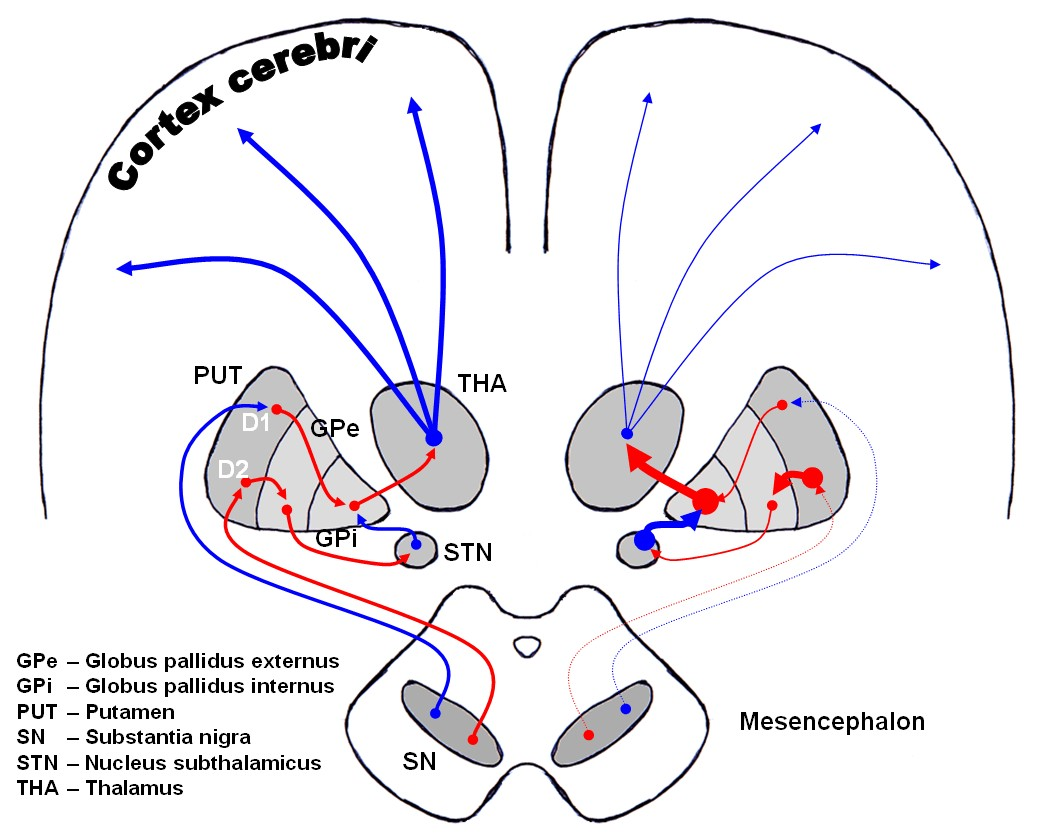
\includegraphics[width=0.5\linewidth]{FileAusiliari/Immagini/degenerative/dopamine-in-parkinsons-disease-illustration}
	\caption[Vie dopaminergiche]{L'immagine mostra le vie dopaminergiche del cervello umano in condizioni normali (a sinistra) e nella malattia di Parkinson (a destra). Le frecce rosse indicano la soppressione del bersaglio, quelle blu la stimolazione della struttura bersaglio. Caso per gentile concessione di Wikipedia, Radiopaedia.org, rID: 36286}
	\label{fig:dopamine-in-parkinsons-disease-illustration}
\end{figure*}

\subsection{Epidemiologia}
Il MP costituisce una delle principali cause di disabilità e mortalità nell'ambito delle patologie neurologiche, con una prevalenza particolarmente elevata negli Stati Uniti e in Canada (160-180 casi/100.000 abitanti). L'incidenza annuale in Nord America oscilla tra 108 e 212 casi ogni 100.000 individui di età $\geq$65 anni, con una prevalenza dello 0,3\% nella popolazione adulta $\geq$40 anni e dell'1,6\% nei soggetti ultrasessantacinquenni.
L'esordio della patologia mostra una significativa correlazione con l'età, manifestandosi tipicamente dalla quinta decade di vita, con un'età media alla diagnosi di 70,5 anni e una finestra di esordio prevalente tra i 45 e i 70 anni. Una variante giovanile può presentarsi tra i 20 e i 40 anni, sebbene l'esordio prima dei 30 anni risulti infrequente. La distribuzione per sesso evidenzia una predominanza maschile, particolarmente accentuata nella fascia d'età 50-60 anni.
L'eziologia del MP comprende fattori di rischio genetici, con particolare rilevanza nelle forme ad esordio precoce, e ambientali, tra cui l'esposizione a pesticidi e inquinanti atmosferici. Sono stati identificati fattori protettivi, inclusi il consumo di caffè, l'attività fisica e il fumo di sigaretta. La patologia si presenta prevalentemente in forma sporadica (85-90\% dei casi), mentre una minoranza dei casi (10-15\%) presenta familiarità positiva.

\subsubsection{Fattori di rischio}
L'eziopatogenesi del Morbo di Parkinson (MP) presenta una complessa interazione di fattori di rischio genetici, ambientali e non modificabili. L'anamnesi familiare positiva per MP in consanguinei di primo grado comporta un incremento del rischio relativo di 2-3 volte. Le forme monogeniche, rappresentanti meno del 10\% della casistica totale, manifestano pattern di ereditarietà autosomica dominante, recessiva o X-linked, caratterizzandosi per un esordio precoce rispetto alle forme sporadiche.
Le mutazioni eterozigoti del gene GBA1 costituiscono un significativo fattore di rischio genetico, unitamente ad alterazioni di altri geni codificanti per enzimi lisosomiali. Il coinvolgimento di geni quali SNCA, LRRK2, VPS35, Parkin, PINK1 e DJ-1 è stato ampiamente documentato. Particolare rilevanza assumono le mutazioni del gene Nurr1, determinante per l'identità neuronale dopaminergica, e del gene DJ-1, cruciale nella risposta allo stress ossidativo. Le alterazioni del gene PINK1, codificante per una chinasi mitocondriale, e del gene Park2, responsabile della sintesi della proteina parkina, sono associate a forme ad esordio precoce.
L'esposizione a neurotossine ambientali, inclusi mercurio, manganese, disolfuro di carbonio, solventi organici, MPTP e monossido di carbonio, può indurre degenerazione nigrostriatale e parkinsonismo. L'uso di neurolettici e l'abuso endovenoso di efedrone possono causare sindromi parkinsoniane potenzialmente irreversibili. Traumi cranici ripetuti, pesticidi, solventi e inquinamento atmosferico rappresentano ulteriori fattori di rischio ambientale documentati.
Tra i fattori non modificabili, l'età avanzata e il sesso maschile emergono come significativi predittori di rischio, con predominanza nella sesta decade di vita. Comorbidità quali depressione, ansia, stipsi, diabete mellito tipo 2, obesità e alterazioni del metabolismo del ferro sono state correlate a un incrementato rischio di MP.
Il consumo di tabacco e caffè, unitamente all'attività fisica regolare, ha mostrato effetti protettivi, sebbene di modesta entità. È fondamentale sottolineare che la maggioranza dei casi di MP rimane idiopatica, suggerendo un'eziologia multifattoriale.

\subsection{Presentazione  clinica}
La sintomatologia del Morbo di Parkinson manifesta un quadro clinico caratterizzato da manifestazioni motorie cardinali e sintomatologia non motoria associata. Il complesso sintomatologico motorio comprende tremore a riposo spesso asimmetrico con frequenza di 4-6 Hz, tipicamente descritto come "pill-rolling", bradicinesia manifestantesi con rallentamento motorio, ipomimia e ridotta oscillazione pendolare degli arti superiori durante la deambulazione, rigidità muscolare ("lead-pipe" o fenomeno della ruota dentata), e instabilità posturale documentabile attraverso il test della retropulsione. La deambulazione risulta caratterizzata da una progressione a piccoli passi con tendenza allo strascicamento e ridotta oscillazione degli arti superiori.
La sintomatologia accessoria include disartria con eloquio esplosivo secondario a incoordinazione linguo-diaframmatica, movimenti involontari della lingua con conseguente difficoltà protrusiva, e incremento della frequenza di ammiccamento palpebrale, quest'ultimo in contrasto con quanto osservato nella corea di Huntington. La disfunzione autonomica, i disturbi olfattivi, la sintomatologia algica, le alterazioni sensitive e i disturbi timici costituiscono il corredo sintomatologico non motorio. Il deterioramento cognitivo, con particolare coinvolgimento delle funzioni attentive, può manifestarsi e progredire nel decorso della patologia.
La progressione temporale della malattia evidenzia un esordio tipicamente unilaterale con successiva bilateralizzazione, manifestandosi prevalentemente nella sesta decade di vita. La responsività alla terapia dopaminergica, in particolare alla levodopa, rappresenta un elemento caratteristico, sebbene il tremore possa risultare farmacoresistente, in contrasto con la significativa risposta della bradicinesia e della rigidità. La variabilità fenotipica interindividuale costituisce un elemento distintivo della patologia.

\subsection{Approccio diagnostico}
L'iter diagnostico della malattia di Parkinson si fonda primariamente sulla valutazione clinica, data l'assenza di biomarcatori patognomonici. La diagnosi richiede la documentazione di bradicinesia associata ad almeno un sintomo cardine tra tremore a riposo o rigidità, valutati mediante la scala MDS-UPDRS standardizzata.
L'approccio diagnostico contempla un'accurata anamnesi ed esame obiettivo neurologico, focalizzati sull'identificazione dei sintomi cardinali: bradicinesia, tremore a riposo (4-6 Hz) tipicamente asimmetrico, rigidità e instabilità posturale. La responsività alla terapia dopaminergica, particolarmente evidente per bradicinesia e rigidità, costituisce un elemento diagnostico supportivo significativo, mentre una mancata risposta a dosaggi adeguati di levodopa suggerisce diagnosi alternative.
L'esclusione di parkinsonismi secondari richiede particolare attenzione all'insorgenza temporale dei sintomi e alla distribuzione topografica del coinvolgimento motorio. La diagnostica per immagini, sebbene non necessaria nelle presentazioni cliniche tipiche con adeguata risposta alla levodopa, può includere RM cerebrale, particolarmente utile mediante sequenze SWI per la valutazione del "swallow tail sign" nigrostriatale. La SPECT con 123I-FP-CIT (DaTscan) documenta la disfunzione dopaminergica presinaptica, mentre la PET con FDG consente la differenziazione metabolica tra PD e sindromi parkinsoniane atipiche.
L'analisi genetica, indicata in casi selezionati (esordio precoce, familiarità positiva, specifiche etnie), e la valutazione autonomica mediante scintigrafia miocardica con MIBG, che evidenzia la denervazione simpatica caratteristica, completano l'iter diagnostico. L'ecografia transcranica può evidenziare l'iperecogenicità della sostanza nera, supportando la diagnosi differenziale.
I criteri MDS stratificano la diagnosi in PD clinicamente stabilita e probabile, bilanciando specificità e sensibilità diagnostica nella pratica clinica.

\begin{Oss}
	La scala MDS-UPDRS (Movement Disorder Society-Unified Parkinson's Disease Rating Scale) è uno strumento di valutazione clinica ampiamente utilizzato per quantificare la gravità dei sintomi motori e non motori della malattia di Parkinson. Questa scala è stata sviluppata per migliorare la consistenza nella valutazione dei sintomi e per integrare meglio gli aspetti non motori della PD.
	Struttura: La scala MDS-UPDRS è composta da quattro sezioni:
	\begin{description}
		\item[Sezione I]{Esperienze non motorie della vita quotidiana. Questa sezione valuta aspetti come le capacità cognitive, i disturbi comportamentali e dell'umore}
		\item [Sezione II]{Esperienze motorie della vita quotidiana. Questa sezione valuta l'impatto dei sintomi motori sulle attività quotidiane}
		\item [Sezione III]{Esame motorio. Questa sezione valuta i segni motori della PD attraverso un esame clinico, come il tremore, la rigidità e la bradicinesia}
		\item[Sezione IV]{Complicanze della terapia. Questa sezione valuta le complicanze associate al trattamento farmacologico}
	\end{description}
	Il punteggio totale per le sezioni I-IV varia da 0 (nessuna disabilità) a 199 (disabilità totale). La sezione III, che valuta i sintomi motori, ha un punteggio che varia da 0 a 132.
	Oltre alla scala MDS-UPDRS, esistono altre scale di valutazione utilizzate nella PD, come la scala di Hoehn e Yahr e la scala di Schwab e England. La scala di Hoehn e Yahr valuta la gravità della malattia da 0 (nessuna malattia) a 5 (paziente costretto su sedia a rotelle o allettato senza assistenza).
\end{Oss}

\subsection{Anatomia patologica}
Dal punto di vista anatomopatologico il morbo di Parkinson si manifesta attraverso inclusioni proteiche intraneuronali denominate corpi di Lewy, costituiti primariamente da aggregati patologici di alfa-sinucleina, una proteina sinaptica fisiologicamente presente nel sistema nervoso centrale. L'accumulo di queste inclusioni, sebbene non patognomonico del morbo di Parkinson essendo documentabile anche nella demenza a corpi di Lewy, rappresenta una caratteristica istopatologica fondamentale quando localizzato nella substantia nigra, in associazione alla perdita neuronale dopaminergica. L'assenza di corpi di Lewy nelle forme post-encefalitiche, caratterizzate invece da grovigli neurofibrillari, e in alcune forme geneticamente determinate, sottolinea l'eterogeneità patogenetica della malattia.
La progressione spazio-temporale della patologia, codificata nello staging di Braak, delinea sei stadi evolutivi caratterizzati da una diffusione ascendente delle alterazioni neuropatologiche. Gli stadi iniziali (1-2) coinvolgono il nucleo motore dorsale dei nervi glossofaringeo e vago e il nucleo olfattivo anteriore, precedendo frequentemente la sintomatologia motoria. Gli stadi intermedi (3-4) documentano il coinvolgimento della substantia nigra pars compacta, del prosencefalo basale e della mesocorteccia temporale, correlando con l'esordio clinico della malattia. Gli stadi terminali (5-6) evidenziano una progressione neocorticale diffusa.
La patogenesi molecolare implica alterazioni del metabolismo dell'alfa-sinucleina, potenzialmente accelerate da disfunzioni delle proteine heat shock o dall'azione della dopamina. Il coinvolgimento della proteina parkin nella degradazione proteasomica evidenzia meccanismi neurodegenerativi potenzialmente indipendenti dalla formazione dei corpi di Lewy.
L'alfa-sinucleina, proteina fisiologicamente localizzata nelle terminazioni presinaptiche neuronali, manifesta nella patogenesi del morbo di Parkinson un processo patologico caratterizzato da misfolding proteico e successiva aggregazione in oligomeri, protofibrille e fibrille, culminante nella formazione dei corpi di Lewy intraneuronali. Questi aggregati proteici, considerati hallmark istopatologico della malattia, evidenziano particolare neurotossicità nella forma protofibrillare, determinando disfunzione e successiva degenerazione neuronale dopaminergica nigrostriatale.
L'identificazione di mutazioni nel gene SNCA, codificante per l'alfa-sinucleina, nelle forme familiari di malattia, unitamente alla documentazione di fenotipi clinici particolarmente aggressivi in presenza di duplicazione o triplicazione genica, ha fornito evidenze significative del ruolo causale di questa proteina nella patogenesi della malattia. La documentata capacità di trasmissione transcellulare dell'alfa-sinucleina patologica costituisce il substrato molecolare della progressione anatomopatologica descritta nello staging di Braak.
La disfunzione sinaptica correlata all'accumulo di alfa-sinucleina rappresenta un meccanismo patogenetico critico, modulato da fattori quali stress ossidativo, alterazioni del sistema ubiquitina-proteasoma e interazione con il metabolismo dopaminergico. Mutazioni nei geni parkin, PINK1 e DJ-1 influenzano il metabolismo dell'alfa-sinucleina attraverso alterazioni dei sistemi di degradazione proteica.
L'alfa-sinucleina costituisce attualmente un promettente target terapeutico, con particolare interesse per lo sviluppo di anticorpi monoclonali specifici e inibitori dell'aggregazione proteica, finalizzati al rallentamento della progressione patologica.

\subsection{Imaging}

\subsubsection{TC}
La TC manifesta un'utilità clinica circoscritta nella valutazione diagnostica primaria del MP, assumendo rilevanza nell'esclusione di patologie strutturali mimiche quali lesioni espansive, idrocefalo o alterazioni vascolari, particolarmente in presenza di presentazioni cliniche atipiche o "red flags" suggestive di diagnosi alternative.
Nel contesto della gestione terapeutica, la TC assume particolare rilevanza nella valutazione post-chirurgica della stimolazione cerebrale profonda (DBS), consentendo la verifica del corretto posizionamento degli elettrodi nel nucleo subtalamico (STN), tipicamente localizzati a 9mm dalla linea mediana, e l'identificazione di eventuali complicanze post-procedurali quali eventi emorragici, ischemici o fenomeni infiammatori transitori, questi ultimi caratterizzati da aree ipodense perilettrodiche a risoluzione graduale. L'utilità della metodica nel follow-up routinario post-DBS risulta secondaria.
La sensibilità subottimale della TC nella diagnosi differenziale tra PD e sindromi parkinsoniane atipiche, incluse atrofia multisistemica e paralisi sopranucleare progressiva, nonché nella distinzione dal tremore essenziale, ne limita significativamente l'applicazione clinica in questo contesto diagnostico.

\subsubsection{RM}
La RM è frequentemente normale nelle sequenze convenzionali (T1, T2, FLAIR) nelle fasi iniziali di malattia. L'implementazione di sequenze susceptibility-weighted imaging (SWI) o T2*-weighted ad alta risoluzione consente la visualizzazione del nigrosoma-1, struttura caratterizzata dal patognomonico "swallow tail sign", la cui perdita correla con la degenerazione dopaminergica nigrostriatale. L'accumulo patologico di ferro nella substantia nigra, quantificabile mediante sequenze SWI/T2* e incrementato del 50\% rispetto ai controlli, costituisce un ulteriore marker diagnostico, complementato dall'imaging della neuromelanina mediante sequenze T1 con impulsi di trasferimento di magnetizzazione (MTC).

\begin{figure*}[h]
	\centering
	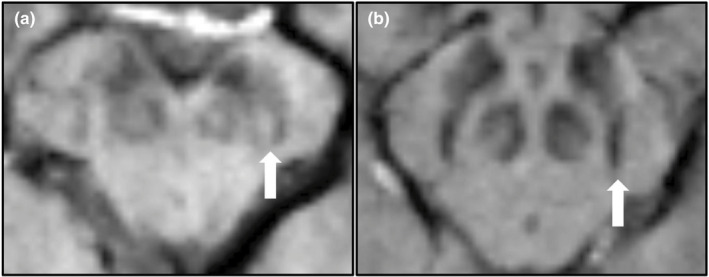
\includegraphics[width=0.8\linewidth]{FileAusiliari/Immagini/degenerative/BRB3-11-e02202-g002}
	\caption{Esempi di segno della coda di rondine (STS) in un individuo malato (a) e di STS assente in un individuo sano (b). Sono mostrate sezioni assiali del mesencefalo mappate tramite imaging pesato con suscettibilità (SWI). Le frecce bianche indicano la diversa configurazione del Nigrosoma-1 (N1). Da Brain Behav. 2021 May 24;11(7):e02202. doi: 10.1002/brb3.2202}
	\label{fig:brb3-11-e02202-g002}
\end{figure*}


La diagnosi differenziale delle sindromi parkinsoniane atipiche beneficia significativamente dell'imaging RM. L'atrofia multisistemica (MSA) evidenzia caratteristica atrofia putaminale, pontica e cerebellare, con ipointensità putaminale T2/SWI e "hot cross bun sign" pontino. La paralisi sopranucleare progressiva (PSP) manifesta atrofia mesencefalica con alterazione del rapporto mesencefalo-ponte, mentre la degenerazione corticobasale (CBD) presenta atrofia frontoparietale asimmetrica con iperintensità della sostanza bianca subcorticale.
Metodiche avanzate quali Diffusion Tensor Imaging (DTI) e risonanza magnetica funzionale (fMRI) consentono la caratterizzazione delle alterazioni microstrutturali della sostanza bianca e delle modificazioni funzionali cerebrali, sebbene la sensibilità nell'identificazione della progressione patologica e nella valutazione della risposta terapeutica necessiti ulteriore validazione. Le limitazioni metodologiche includono variabilità interindividuale e sovrapposizione dei reperti radiologici nelle diverse sindromi parkinsoniane.

\subsection{Trattamento e prognosi}

\subsection{Checklist di refertazione}

\begin{itemize}[label=$\square$] % Riquadro vuoto come simbolo
	\item Escludi altre cause di parkinsonismo (es ictus)
	\item Controlla il segnale dei nigrosomi
	\item Controlla il trofismo delle strutture sottotentoriali
\end{itemize}

\subsection{Bibliografia}
\small{
	
	
}

\note{Nota a margine}
\expl{Nota a margine colorata}
\input{Capitoli/degenerative/approccio.tex}
\input{Capitoli/degenerative/degenerative.tex}
\section{Morbo di Parkinson}

\subsection{Definizione}

\subsection{Eziologia}

\begin{figure*}[h]
	\centering
	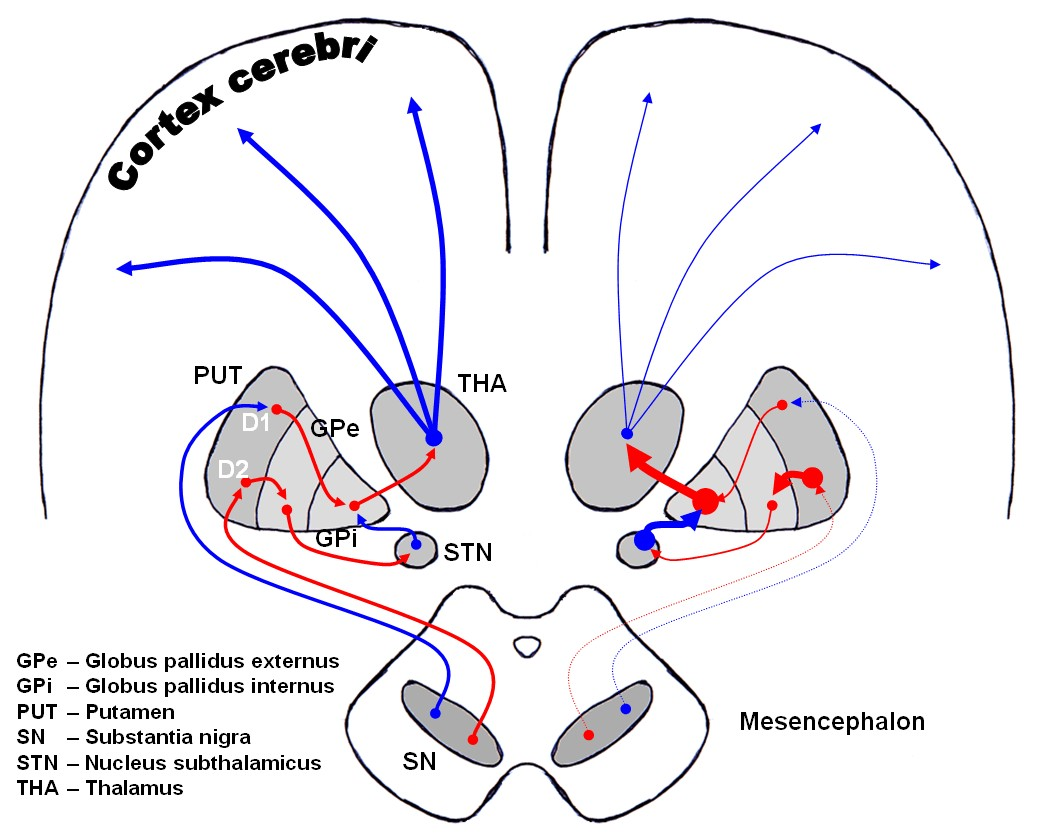
\includegraphics[width=0.5\linewidth]{FileAusiliari/Immagini/degenerative/dopamine-in-parkinsons-disease-illustration}
	\caption[Vie dopaminergiche]{L'immagine mostra le vie dopaminergiche del cervello umano in condizioni normali (a sinistra) e nella malattia di Parkinson (a destra). Le frecce rosse indicano la soppressione del bersaglio, quelle blu la stimolazione della struttura bersaglio. Caso per gentile concessione di Wikipedia, Radiopaedia.org, rID: 36286}
	\label{fig:dopamine-in-parkinsons-disease-illustration}
\end{figure*}

\subsection{Epidemiologia}
Il MP costituisce una delle principali cause di disabilità e mortalità nell'ambito delle patologie neurologiche, con una prevalenza particolarmente elevata negli Stati Uniti e in Canada (160-180 casi/100.000 abitanti). L'incidenza annuale in Nord America oscilla tra 108 e 212 casi ogni 100.000 individui di età $\geq$65 anni, con una prevalenza dello 0,3\% nella popolazione adulta $\geq$40 anni e dell'1,6\% nei soggetti ultrasessantacinquenni.
L'esordio della patologia mostra una significativa correlazione con l'età, manifestandosi tipicamente dalla quinta decade di vita, con un'età media alla diagnosi di 70,5 anni e una finestra di esordio prevalente tra i 45 e i 70 anni. Una variante giovanile può presentarsi tra i 20 e i 40 anni, sebbene l'esordio prima dei 30 anni risulti infrequente. La distribuzione per sesso evidenzia una predominanza maschile, particolarmente accentuata nella fascia d'età 50-60 anni.
L'eziologia del MP comprende fattori di rischio genetici, con particolare rilevanza nelle forme ad esordio precoce, e ambientali, tra cui l'esposizione a pesticidi e inquinanti atmosferici. Sono stati identificati fattori protettivi, inclusi il consumo di caffè, l'attività fisica e il fumo di sigaretta. La patologia si presenta prevalentemente in forma sporadica (85-90\% dei casi), mentre una minoranza dei casi (10-15\%) presenta familiarità positiva.

\subsubsection{Fattori di rischio}
L'eziopatogenesi del Morbo di Parkinson (MP) presenta una complessa interazione di fattori di rischio genetici, ambientali e non modificabili. L'anamnesi familiare positiva per MP in consanguinei di primo grado comporta un incremento del rischio relativo di 2-3 volte. Le forme monogeniche, rappresentanti meno del 10\% della casistica totale, manifestano pattern di ereditarietà autosomica dominante, recessiva o X-linked, caratterizzandosi per un esordio precoce rispetto alle forme sporadiche.
Le mutazioni eterozigoti del gene GBA1 costituiscono un significativo fattore di rischio genetico, unitamente ad alterazioni di altri geni codificanti per enzimi lisosomiali. Il coinvolgimento di geni quali SNCA, LRRK2, VPS35, Parkin, PINK1 e DJ-1 è stato ampiamente documentato. Particolare rilevanza assumono le mutazioni del gene Nurr1, determinante per l'identità neuronale dopaminergica, e del gene DJ-1, cruciale nella risposta allo stress ossidativo. Le alterazioni del gene PINK1, codificante per una chinasi mitocondriale, e del gene Park2, responsabile della sintesi della proteina parkina, sono associate a forme ad esordio precoce.
L'esposizione a neurotossine ambientali, inclusi mercurio, manganese, disolfuro di carbonio, solventi organici, MPTP e monossido di carbonio, può indurre degenerazione nigrostriatale e parkinsonismo. L'uso di neurolettici e l'abuso endovenoso di efedrone possono causare sindromi parkinsoniane potenzialmente irreversibili. Traumi cranici ripetuti, pesticidi, solventi e inquinamento atmosferico rappresentano ulteriori fattori di rischio ambientale documentati.
Tra i fattori non modificabili, l'età avanzata e il sesso maschile emergono come significativi predittori di rischio, con predominanza nella sesta decade di vita. Comorbidità quali depressione, ansia, stipsi, diabete mellito tipo 2, obesità e alterazioni del metabolismo del ferro sono state correlate a un incrementato rischio di MP.
Il consumo di tabacco e caffè, unitamente all'attività fisica regolare, ha mostrato effetti protettivi, sebbene di modesta entità. È fondamentale sottolineare che la maggioranza dei casi di MP rimane idiopatica, suggerendo un'eziologia multifattoriale.

\subsection{Presentazione  clinica}
La sintomatologia del Morbo di Parkinson manifesta un quadro clinico caratterizzato da manifestazioni motorie cardinali e sintomatologia non motoria associata. Il complesso sintomatologico motorio comprende tremore a riposo spesso asimmetrico con frequenza di 4-6 Hz, tipicamente descritto come "pill-rolling", bradicinesia manifestantesi con rallentamento motorio, ipomimia e ridotta oscillazione pendolare degli arti superiori durante la deambulazione, rigidità muscolare ("lead-pipe" o fenomeno della ruota dentata), e instabilità posturale documentabile attraverso il test della retropulsione. La deambulazione risulta caratterizzata da una progressione a piccoli passi con tendenza allo strascicamento e ridotta oscillazione degli arti superiori.
La sintomatologia accessoria include disartria con eloquio esplosivo secondario a incoordinazione linguo-diaframmatica, movimenti involontari della lingua con conseguente difficoltà protrusiva, e incremento della frequenza di ammiccamento palpebrale, quest'ultimo in contrasto con quanto osservato nella corea di Huntington. La disfunzione autonomica, i disturbi olfattivi, la sintomatologia algica, le alterazioni sensitive e i disturbi timici costituiscono il corredo sintomatologico non motorio. Il deterioramento cognitivo, con particolare coinvolgimento delle funzioni attentive, può manifestarsi e progredire nel decorso della patologia.
La progressione temporale della malattia evidenzia un esordio tipicamente unilaterale con successiva bilateralizzazione, manifestandosi prevalentemente nella sesta decade di vita. La responsività alla terapia dopaminergica, in particolare alla levodopa, rappresenta un elemento caratteristico, sebbene il tremore possa risultare farmacoresistente, in contrasto con la significativa risposta della bradicinesia e della rigidità. La variabilità fenotipica interindividuale costituisce un elemento distintivo della patologia.

\subsection{Approccio diagnostico}
L'iter diagnostico della malattia di Parkinson si fonda primariamente sulla valutazione clinica, data l'assenza di biomarcatori patognomonici. La diagnosi richiede la documentazione di bradicinesia associata ad almeno un sintomo cardine tra tremore a riposo o rigidità, valutati mediante la scala MDS-UPDRS standardizzata.
L'approccio diagnostico contempla un'accurata anamnesi ed esame obiettivo neurologico, focalizzati sull'identificazione dei sintomi cardinali: bradicinesia, tremore a riposo (4-6 Hz) tipicamente asimmetrico, rigidità e instabilità posturale. La responsività alla terapia dopaminergica, particolarmente evidente per bradicinesia e rigidità, costituisce un elemento diagnostico supportivo significativo, mentre una mancata risposta a dosaggi adeguati di levodopa suggerisce diagnosi alternative.
L'esclusione di parkinsonismi secondari richiede particolare attenzione all'insorgenza temporale dei sintomi e alla distribuzione topografica del coinvolgimento motorio. La diagnostica per immagini, sebbene non necessaria nelle presentazioni cliniche tipiche con adeguata risposta alla levodopa, può includere RM cerebrale, particolarmente utile mediante sequenze SWI per la valutazione del "swallow tail sign" nigrostriatale. La SPECT con 123I-FP-CIT (DaTscan) documenta la disfunzione dopaminergica presinaptica, mentre la PET con FDG consente la differenziazione metabolica tra PD e sindromi parkinsoniane atipiche.
L'analisi genetica, indicata in casi selezionati (esordio precoce, familiarità positiva, specifiche etnie), e la valutazione autonomica mediante scintigrafia miocardica con MIBG, che evidenzia la denervazione simpatica caratteristica, completano l'iter diagnostico. L'ecografia transcranica può evidenziare l'iperecogenicità della sostanza nera, supportando la diagnosi differenziale.
I criteri MDS stratificano la diagnosi in PD clinicamente stabilita e probabile, bilanciando specificità e sensibilità diagnostica nella pratica clinica.

\begin{Oss}
	La scala MDS-UPDRS (Movement Disorder Society-Unified Parkinson's Disease Rating Scale) è uno strumento di valutazione clinica ampiamente utilizzato per quantificare la gravità dei sintomi motori e non motori della malattia di Parkinson. Questa scala è stata sviluppata per migliorare la consistenza nella valutazione dei sintomi e per integrare meglio gli aspetti non motori della PD.
	Struttura: La scala MDS-UPDRS è composta da quattro sezioni:
	\begin{description}
		\item[Sezione I]{Esperienze non motorie della vita quotidiana. Questa sezione valuta aspetti come le capacità cognitive, i disturbi comportamentali e dell'umore}
		\item [Sezione II]{Esperienze motorie della vita quotidiana. Questa sezione valuta l'impatto dei sintomi motori sulle attività quotidiane}
		\item [Sezione III]{Esame motorio. Questa sezione valuta i segni motori della PD attraverso un esame clinico, come il tremore, la rigidità e la bradicinesia}
		\item[Sezione IV]{Complicanze della terapia. Questa sezione valuta le complicanze associate al trattamento farmacologico}
	\end{description}
	Il punteggio totale per le sezioni I-IV varia da 0 (nessuna disabilità) a 199 (disabilità totale). La sezione III, che valuta i sintomi motori, ha un punteggio che varia da 0 a 132.
	Oltre alla scala MDS-UPDRS, esistono altre scale di valutazione utilizzate nella PD, come la scala di Hoehn e Yahr e la scala di Schwab e England. La scala di Hoehn e Yahr valuta la gravità della malattia da 0 (nessuna malattia) a 5 (paziente costretto su sedia a rotelle o allettato senza assistenza).
\end{Oss}

\subsection{Anatomia patologica}
Dal punto di vista anatomopatologico il morbo di Parkinson si manifesta attraverso inclusioni proteiche intraneuronali denominate corpi di Lewy, costituiti primariamente da aggregati patologici di alfa-sinucleina, una proteina sinaptica fisiologicamente presente nel sistema nervoso centrale. L'accumulo di queste inclusioni, sebbene non patognomonico del morbo di Parkinson essendo documentabile anche nella demenza a corpi di Lewy, rappresenta una caratteristica istopatologica fondamentale quando localizzato nella substantia nigra, in associazione alla perdita neuronale dopaminergica. L'assenza di corpi di Lewy nelle forme post-encefalitiche, caratterizzate invece da grovigli neurofibrillari, e in alcune forme geneticamente determinate, sottolinea l'eterogeneità patogenetica della malattia.
La progressione spazio-temporale della patologia, codificata nello staging di Braak, delinea sei stadi evolutivi caratterizzati da una diffusione ascendente delle alterazioni neuropatologiche. Gli stadi iniziali (1-2) coinvolgono il nucleo motore dorsale dei nervi glossofaringeo e vago e il nucleo olfattivo anteriore, precedendo frequentemente la sintomatologia motoria. Gli stadi intermedi (3-4) documentano il coinvolgimento della substantia nigra pars compacta, del prosencefalo basale e della mesocorteccia temporale, correlando con l'esordio clinico della malattia. Gli stadi terminali (5-6) evidenziano una progressione neocorticale diffusa.
La patogenesi molecolare implica alterazioni del metabolismo dell'alfa-sinucleina, potenzialmente accelerate da disfunzioni delle proteine heat shock o dall'azione della dopamina. Il coinvolgimento della proteina parkin nella degradazione proteasomica evidenzia meccanismi neurodegenerativi potenzialmente indipendenti dalla formazione dei corpi di Lewy.
L'alfa-sinucleina, proteina fisiologicamente localizzata nelle terminazioni presinaptiche neuronali, manifesta nella patogenesi del morbo di Parkinson un processo patologico caratterizzato da misfolding proteico e successiva aggregazione in oligomeri, protofibrille e fibrille, culminante nella formazione dei corpi di Lewy intraneuronali. Questi aggregati proteici, considerati hallmark istopatologico della malattia, evidenziano particolare neurotossicità nella forma protofibrillare, determinando disfunzione e successiva degenerazione neuronale dopaminergica nigrostriatale.
L'identificazione di mutazioni nel gene SNCA, codificante per l'alfa-sinucleina, nelle forme familiari di malattia, unitamente alla documentazione di fenotipi clinici particolarmente aggressivi in presenza di duplicazione o triplicazione genica, ha fornito evidenze significative del ruolo causale di questa proteina nella patogenesi della malattia. La documentata capacità di trasmissione transcellulare dell'alfa-sinucleina patologica costituisce il substrato molecolare della progressione anatomopatologica descritta nello staging di Braak.
La disfunzione sinaptica correlata all'accumulo di alfa-sinucleina rappresenta un meccanismo patogenetico critico, modulato da fattori quali stress ossidativo, alterazioni del sistema ubiquitina-proteasoma e interazione con il metabolismo dopaminergico. Mutazioni nei geni parkin, PINK1 e DJ-1 influenzano il metabolismo dell'alfa-sinucleina attraverso alterazioni dei sistemi di degradazione proteica.
L'alfa-sinucleina costituisce attualmente un promettente target terapeutico, con particolare interesse per lo sviluppo di anticorpi monoclonali specifici e inibitori dell'aggregazione proteica, finalizzati al rallentamento della progressione patologica.

\subsection{Imaging}

\subsubsection{TC}
La TC manifesta un'utilità clinica circoscritta nella valutazione diagnostica primaria del MP, assumendo rilevanza nell'esclusione di patologie strutturali mimiche quali lesioni espansive, idrocefalo o alterazioni vascolari, particolarmente in presenza di presentazioni cliniche atipiche o "red flags" suggestive di diagnosi alternative.
Nel contesto della gestione terapeutica, la TC assume particolare rilevanza nella valutazione post-chirurgica della stimolazione cerebrale profonda (DBS), consentendo la verifica del corretto posizionamento degli elettrodi nel nucleo subtalamico (STN), tipicamente localizzati a 9mm dalla linea mediana, e l'identificazione di eventuali complicanze post-procedurali quali eventi emorragici, ischemici o fenomeni infiammatori transitori, questi ultimi caratterizzati da aree ipodense perilettrodiche a risoluzione graduale. L'utilità della metodica nel follow-up routinario post-DBS risulta secondaria.
La sensibilità subottimale della TC nella diagnosi differenziale tra PD e sindromi parkinsoniane atipiche, incluse atrofia multisistemica e paralisi sopranucleare progressiva, nonché nella distinzione dal tremore essenziale, ne limita significativamente l'applicazione clinica in questo contesto diagnostico.

\subsubsection{RM}
La RM è frequentemente normale nelle sequenze convenzionali (T1, T2, FLAIR) nelle fasi iniziali di malattia. L'implementazione di sequenze susceptibility-weighted imaging (SWI) o T2*-weighted ad alta risoluzione consente la visualizzazione del nigrosoma-1, struttura caratterizzata dal patognomonico "swallow tail sign", la cui perdita correla con la degenerazione dopaminergica nigrostriatale. L'accumulo patologico di ferro nella substantia nigra, quantificabile mediante sequenze SWI/T2* e incrementato del 50\% rispetto ai controlli, costituisce un ulteriore marker diagnostico, complementato dall'imaging della neuromelanina mediante sequenze T1 con impulsi di trasferimento di magnetizzazione (MTC).

\begin{figure*}[h]
	\centering
	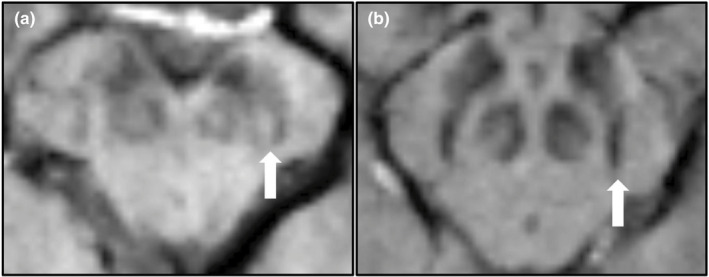
\includegraphics[width=0.8\linewidth]{FileAusiliari/Immagini/degenerative/BRB3-11-e02202-g002}
	\caption{Esempi di segno della coda di rondine (STS) in un individuo malato (a) e di STS assente in un individuo sano (b). Sono mostrate sezioni assiali del mesencefalo mappate tramite imaging pesato con suscettibilità (SWI). Le frecce bianche indicano la diversa configurazione del Nigrosoma-1 (N1). Da Brain Behav. 2021 May 24;11(7):e02202. doi: 10.1002/brb3.2202}
	\label{fig:brb3-11-e02202-g002}
\end{figure*}


La diagnosi differenziale delle sindromi parkinsoniane atipiche beneficia significativamente dell'imaging RM. L'atrofia multisistemica (MSA) evidenzia caratteristica atrofia putaminale, pontica e cerebellare, con ipointensità putaminale T2/SWI e "hot cross bun sign" pontino. La paralisi sopranucleare progressiva (PSP) manifesta atrofia mesencefalica con alterazione del rapporto mesencefalo-ponte, mentre la degenerazione corticobasale (CBD) presenta atrofia frontoparietale asimmetrica con iperintensità della sostanza bianca subcorticale.
Metodiche avanzate quali Diffusion Tensor Imaging (DTI) e risonanza magnetica funzionale (fMRI) consentono la caratterizzazione delle alterazioni microstrutturali della sostanza bianca e delle modificazioni funzionali cerebrali, sebbene la sensibilità nell'identificazione della progressione patologica e nella valutazione della risposta terapeutica necessiti ulteriore validazione. Le limitazioni metodologiche includono variabilità interindividuale e sovrapposizione dei reperti radiologici nelle diverse sindromi parkinsoniane.

\subsection{Trattamento e prognosi}

\subsection{Checklist di refertazione}

\begin{itemize}[label=$\square$] % Riquadro vuoto come simbolo
	\item Escludi altre cause di parkinsonismo (es ictus)
	\item Controlla il segnale dei nigrosomi
	\item Controlla il trofismo delle strutture sottotentoriali
\end{itemize}

\subsection{Bibliografia}
\small{
	
	
}

\note{Nota a margine}
\expl{Nota a margine colorata}
\input{Capitoli/degenerative/approccio.tex}
\input{Capitoli/degenerative/degenerative.tex}
\section{Morbo di Parkinson}

\subsection{Definizione}

\subsection{Eziologia}

\begin{figure*}[h]
	\centering
	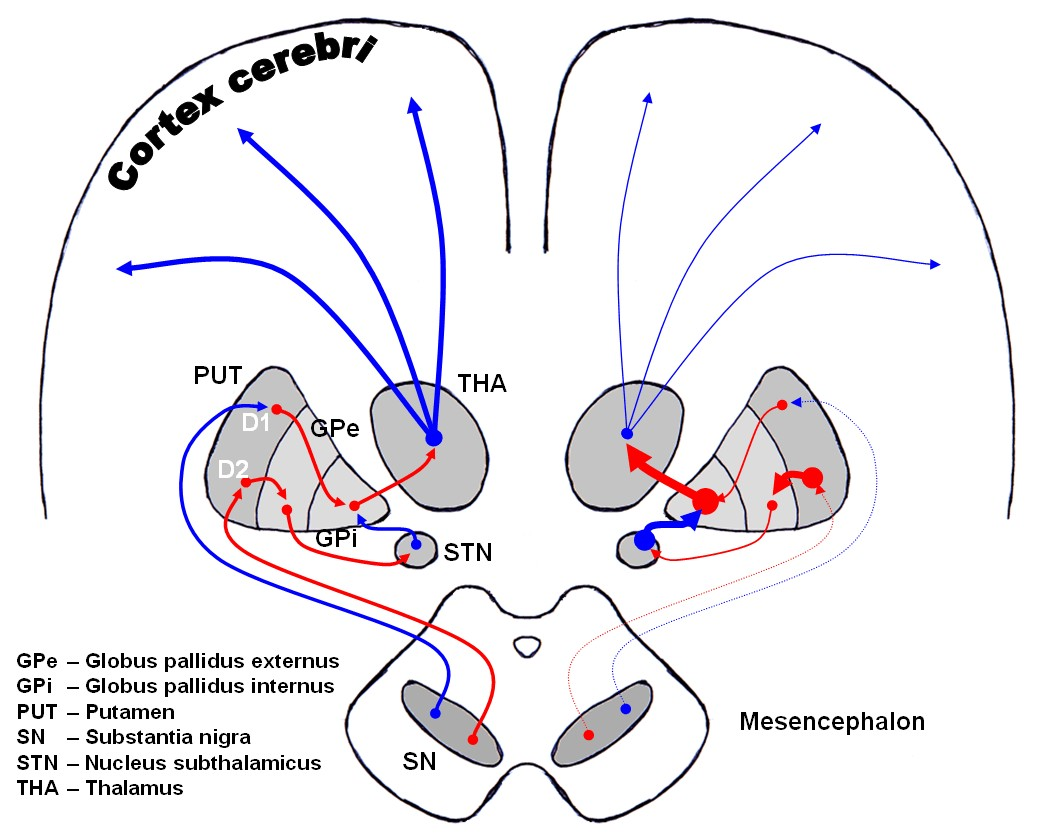
\includegraphics[width=0.5\linewidth]{FileAusiliari/Immagini/degenerative/dopamine-in-parkinsons-disease-illustration}
	\caption[Vie dopaminergiche]{L'immagine mostra le vie dopaminergiche del cervello umano in condizioni normali (a sinistra) e nella malattia di Parkinson (a destra). Le frecce rosse indicano la soppressione del bersaglio, quelle blu la stimolazione della struttura bersaglio. Caso per gentile concessione di Wikipedia, Radiopaedia.org, rID: 36286}
	\label{fig:dopamine-in-parkinsons-disease-illustration}
\end{figure*}

\subsection{Epidemiologia}
Il MP costituisce una delle principali cause di disabilità e mortalità nell'ambito delle patologie neurologiche, con una prevalenza particolarmente elevata negli Stati Uniti e in Canada (160-180 casi/100.000 abitanti). L'incidenza annuale in Nord America oscilla tra 108 e 212 casi ogni 100.000 individui di età $\geq$65 anni, con una prevalenza dello 0,3\% nella popolazione adulta $\geq$40 anni e dell'1,6\% nei soggetti ultrasessantacinquenni.
L'esordio della patologia mostra una significativa correlazione con l'età, manifestandosi tipicamente dalla quinta decade di vita, con un'età media alla diagnosi di 70,5 anni e una finestra di esordio prevalente tra i 45 e i 70 anni. Una variante giovanile può presentarsi tra i 20 e i 40 anni, sebbene l'esordio prima dei 30 anni risulti infrequente. La distribuzione per sesso evidenzia una predominanza maschile, particolarmente accentuata nella fascia d'età 50-60 anni.
L'eziologia del MP comprende fattori di rischio genetici, con particolare rilevanza nelle forme ad esordio precoce, e ambientali, tra cui l'esposizione a pesticidi e inquinanti atmosferici. Sono stati identificati fattori protettivi, inclusi il consumo di caffè, l'attività fisica e il fumo di sigaretta. La patologia si presenta prevalentemente in forma sporadica (85-90\% dei casi), mentre una minoranza dei casi (10-15\%) presenta familiarità positiva.

\subsubsection{Fattori di rischio}
L'eziopatogenesi del Morbo di Parkinson (MP) presenta una complessa interazione di fattori di rischio genetici, ambientali e non modificabili. L'anamnesi familiare positiva per MP in consanguinei di primo grado comporta un incremento del rischio relativo di 2-3 volte. Le forme monogeniche, rappresentanti meno del 10\% della casistica totale, manifestano pattern di ereditarietà autosomica dominante, recessiva o X-linked, caratterizzandosi per un esordio precoce rispetto alle forme sporadiche.
Le mutazioni eterozigoti del gene GBA1 costituiscono un significativo fattore di rischio genetico, unitamente ad alterazioni di altri geni codificanti per enzimi lisosomiali. Il coinvolgimento di geni quali SNCA, LRRK2, VPS35, Parkin, PINK1 e DJ-1 è stato ampiamente documentato. Particolare rilevanza assumono le mutazioni del gene Nurr1, determinante per l'identità neuronale dopaminergica, e del gene DJ-1, cruciale nella risposta allo stress ossidativo. Le alterazioni del gene PINK1, codificante per una chinasi mitocondriale, e del gene Park2, responsabile della sintesi della proteina parkina, sono associate a forme ad esordio precoce.
L'esposizione a neurotossine ambientali, inclusi mercurio, manganese, disolfuro di carbonio, solventi organici, MPTP e monossido di carbonio, può indurre degenerazione nigrostriatale e parkinsonismo. L'uso di neurolettici e l'abuso endovenoso di efedrone possono causare sindromi parkinsoniane potenzialmente irreversibili. Traumi cranici ripetuti, pesticidi, solventi e inquinamento atmosferico rappresentano ulteriori fattori di rischio ambientale documentati.
Tra i fattori non modificabili, l'età avanzata e il sesso maschile emergono come significativi predittori di rischio, con predominanza nella sesta decade di vita. Comorbidità quali depressione, ansia, stipsi, diabete mellito tipo 2, obesità e alterazioni del metabolismo del ferro sono state correlate a un incrementato rischio di MP.
Il consumo di tabacco e caffè, unitamente all'attività fisica regolare, ha mostrato effetti protettivi, sebbene di modesta entità. È fondamentale sottolineare che la maggioranza dei casi di MP rimane idiopatica, suggerendo un'eziologia multifattoriale.

\subsection{Presentazione  clinica}
La sintomatologia del Morbo di Parkinson manifesta un quadro clinico caratterizzato da manifestazioni motorie cardinali e sintomatologia non motoria associata. Il complesso sintomatologico motorio comprende tremore a riposo spesso asimmetrico con frequenza di 4-6 Hz, tipicamente descritto come "pill-rolling", bradicinesia manifestantesi con rallentamento motorio, ipomimia e ridotta oscillazione pendolare degli arti superiori durante la deambulazione, rigidità muscolare ("lead-pipe" o fenomeno della ruota dentata), e instabilità posturale documentabile attraverso il test della retropulsione. La deambulazione risulta caratterizzata da una progressione a piccoli passi con tendenza allo strascicamento e ridotta oscillazione degli arti superiori.
La sintomatologia accessoria include disartria con eloquio esplosivo secondario a incoordinazione linguo-diaframmatica, movimenti involontari della lingua con conseguente difficoltà protrusiva, e incremento della frequenza di ammiccamento palpebrale, quest'ultimo in contrasto con quanto osservato nella corea di Huntington. La disfunzione autonomica, i disturbi olfattivi, la sintomatologia algica, le alterazioni sensitive e i disturbi timici costituiscono il corredo sintomatologico non motorio. Il deterioramento cognitivo, con particolare coinvolgimento delle funzioni attentive, può manifestarsi e progredire nel decorso della patologia.
La progressione temporale della malattia evidenzia un esordio tipicamente unilaterale con successiva bilateralizzazione, manifestandosi prevalentemente nella sesta decade di vita. La responsività alla terapia dopaminergica, in particolare alla levodopa, rappresenta un elemento caratteristico, sebbene il tremore possa risultare farmacoresistente, in contrasto con la significativa risposta della bradicinesia e della rigidità. La variabilità fenotipica interindividuale costituisce un elemento distintivo della patologia.

\subsection{Approccio diagnostico}
L'iter diagnostico della malattia di Parkinson si fonda primariamente sulla valutazione clinica, data l'assenza di biomarcatori patognomonici. La diagnosi richiede la documentazione di bradicinesia associata ad almeno un sintomo cardine tra tremore a riposo o rigidità, valutati mediante la scala MDS-UPDRS standardizzata.
L'approccio diagnostico contempla un'accurata anamnesi ed esame obiettivo neurologico, focalizzati sull'identificazione dei sintomi cardinali: bradicinesia, tremore a riposo (4-6 Hz) tipicamente asimmetrico, rigidità e instabilità posturale. La responsività alla terapia dopaminergica, particolarmente evidente per bradicinesia e rigidità, costituisce un elemento diagnostico supportivo significativo, mentre una mancata risposta a dosaggi adeguati di levodopa suggerisce diagnosi alternative.
L'esclusione di parkinsonismi secondari richiede particolare attenzione all'insorgenza temporale dei sintomi e alla distribuzione topografica del coinvolgimento motorio. La diagnostica per immagini, sebbene non necessaria nelle presentazioni cliniche tipiche con adeguata risposta alla levodopa, può includere RM cerebrale, particolarmente utile mediante sequenze SWI per la valutazione del "swallow tail sign" nigrostriatale. La SPECT con 123I-FP-CIT (DaTscan) documenta la disfunzione dopaminergica presinaptica, mentre la PET con FDG consente la differenziazione metabolica tra PD e sindromi parkinsoniane atipiche.
L'analisi genetica, indicata in casi selezionati (esordio precoce, familiarità positiva, specifiche etnie), e la valutazione autonomica mediante scintigrafia miocardica con MIBG, che evidenzia la denervazione simpatica caratteristica, completano l'iter diagnostico. L'ecografia transcranica può evidenziare l'iperecogenicità della sostanza nera, supportando la diagnosi differenziale.
I criteri MDS stratificano la diagnosi in PD clinicamente stabilita e probabile, bilanciando specificità e sensibilità diagnostica nella pratica clinica.

\begin{Oss}
	La scala MDS-UPDRS (Movement Disorder Society-Unified Parkinson's Disease Rating Scale) è uno strumento di valutazione clinica ampiamente utilizzato per quantificare la gravità dei sintomi motori e non motori della malattia di Parkinson. Questa scala è stata sviluppata per migliorare la consistenza nella valutazione dei sintomi e per integrare meglio gli aspetti non motori della PD.
	Struttura: La scala MDS-UPDRS è composta da quattro sezioni:
	\begin{description}
		\item[Sezione I]{Esperienze non motorie della vita quotidiana. Questa sezione valuta aspetti come le capacità cognitive, i disturbi comportamentali e dell'umore}
		\item [Sezione II]{Esperienze motorie della vita quotidiana. Questa sezione valuta l'impatto dei sintomi motori sulle attività quotidiane}
		\item [Sezione III]{Esame motorio. Questa sezione valuta i segni motori della PD attraverso un esame clinico, come il tremore, la rigidità e la bradicinesia}
		\item[Sezione IV]{Complicanze della terapia. Questa sezione valuta le complicanze associate al trattamento farmacologico}
	\end{description}
	Il punteggio totale per le sezioni I-IV varia da 0 (nessuna disabilità) a 199 (disabilità totale). La sezione III, che valuta i sintomi motori, ha un punteggio che varia da 0 a 132.
	Oltre alla scala MDS-UPDRS, esistono altre scale di valutazione utilizzate nella PD, come la scala di Hoehn e Yahr e la scala di Schwab e England. La scala di Hoehn e Yahr valuta la gravità della malattia da 0 (nessuna malattia) a 5 (paziente costretto su sedia a rotelle o allettato senza assistenza).
\end{Oss}

\subsection{Anatomia patologica}
Dal punto di vista anatomopatologico il morbo di Parkinson si manifesta attraverso inclusioni proteiche intraneuronali denominate corpi di Lewy, costituiti primariamente da aggregati patologici di alfa-sinucleina, una proteina sinaptica fisiologicamente presente nel sistema nervoso centrale. L'accumulo di queste inclusioni, sebbene non patognomonico del morbo di Parkinson essendo documentabile anche nella demenza a corpi di Lewy, rappresenta una caratteristica istopatologica fondamentale quando localizzato nella substantia nigra, in associazione alla perdita neuronale dopaminergica. L'assenza di corpi di Lewy nelle forme post-encefalitiche, caratterizzate invece da grovigli neurofibrillari, e in alcune forme geneticamente determinate, sottolinea l'eterogeneità patogenetica della malattia.
La progressione spazio-temporale della patologia, codificata nello staging di Braak, delinea sei stadi evolutivi caratterizzati da una diffusione ascendente delle alterazioni neuropatologiche. Gli stadi iniziali (1-2) coinvolgono il nucleo motore dorsale dei nervi glossofaringeo e vago e il nucleo olfattivo anteriore, precedendo frequentemente la sintomatologia motoria. Gli stadi intermedi (3-4) documentano il coinvolgimento della substantia nigra pars compacta, del prosencefalo basale e della mesocorteccia temporale, correlando con l'esordio clinico della malattia. Gli stadi terminali (5-6) evidenziano una progressione neocorticale diffusa.
La patogenesi molecolare implica alterazioni del metabolismo dell'alfa-sinucleina, potenzialmente accelerate da disfunzioni delle proteine heat shock o dall'azione della dopamina. Il coinvolgimento della proteina parkin nella degradazione proteasomica evidenzia meccanismi neurodegenerativi potenzialmente indipendenti dalla formazione dei corpi di Lewy.
L'alfa-sinucleina, proteina fisiologicamente localizzata nelle terminazioni presinaptiche neuronali, manifesta nella patogenesi del morbo di Parkinson un processo patologico caratterizzato da misfolding proteico e successiva aggregazione in oligomeri, protofibrille e fibrille, culminante nella formazione dei corpi di Lewy intraneuronali. Questi aggregati proteici, considerati hallmark istopatologico della malattia, evidenziano particolare neurotossicità nella forma protofibrillare, determinando disfunzione e successiva degenerazione neuronale dopaminergica nigrostriatale.
L'identificazione di mutazioni nel gene SNCA, codificante per l'alfa-sinucleina, nelle forme familiari di malattia, unitamente alla documentazione di fenotipi clinici particolarmente aggressivi in presenza di duplicazione o triplicazione genica, ha fornito evidenze significative del ruolo causale di questa proteina nella patogenesi della malattia. La documentata capacità di trasmissione transcellulare dell'alfa-sinucleina patologica costituisce il substrato molecolare della progressione anatomopatologica descritta nello staging di Braak.
La disfunzione sinaptica correlata all'accumulo di alfa-sinucleina rappresenta un meccanismo patogenetico critico, modulato da fattori quali stress ossidativo, alterazioni del sistema ubiquitina-proteasoma e interazione con il metabolismo dopaminergico. Mutazioni nei geni parkin, PINK1 e DJ-1 influenzano il metabolismo dell'alfa-sinucleina attraverso alterazioni dei sistemi di degradazione proteica.
L'alfa-sinucleina costituisce attualmente un promettente target terapeutico, con particolare interesse per lo sviluppo di anticorpi monoclonali specifici e inibitori dell'aggregazione proteica, finalizzati al rallentamento della progressione patologica.

\subsection{Imaging}

\subsubsection{TC}
La TC manifesta un'utilità clinica circoscritta nella valutazione diagnostica primaria del MP, assumendo rilevanza nell'esclusione di patologie strutturali mimiche quali lesioni espansive, idrocefalo o alterazioni vascolari, particolarmente in presenza di presentazioni cliniche atipiche o "red flags" suggestive di diagnosi alternative.
Nel contesto della gestione terapeutica, la TC assume particolare rilevanza nella valutazione post-chirurgica della stimolazione cerebrale profonda (DBS), consentendo la verifica del corretto posizionamento degli elettrodi nel nucleo subtalamico (STN), tipicamente localizzati a 9mm dalla linea mediana, e l'identificazione di eventuali complicanze post-procedurali quali eventi emorragici, ischemici o fenomeni infiammatori transitori, questi ultimi caratterizzati da aree ipodense perilettrodiche a risoluzione graduale. L'utilità della metodica nel follow-up routinario post-DBS risulta secondaria.
La sensibilità subottimale della TC nella diagnosi differenziale tra PD e sindromi parkinsoniane atipiche, incluse atrofia multisistemica e paralisi sopranucleare progressiva, nonché nella distinzione dal tremore essenziale, ne limita significativamente l'applicazione clinica in questo contesto diagnostico.

\subsubsection{RM}
La RM è frequentemente normale nelle sequenze convenzionali (T1, T2, FLAIR) nelle fasi iniziali di malattia. L'implementazione di sequenze susceptibility-weighted imaging (SWI) o T2*-weighted ad alta risoluzione consente la visualizzazione del nigrosoma-1, struttura caratterizzata dal patognomonico "swallow tail sign", la cui perdita correla con la degenerazione dopaminergica nigrostriatale. L'accumulo patologico di ferro nella substantia nigra, quantificabile mediante sequenze SWI/T2* e incrementato del 50\% rispetto ai controlli, costituisce un ulteriore marker diagnostico, complementato dall'imaging della neuromelanina mediante sequenze T1 con impulsi di trasferimento di magnetizzazione (MTC).

\begin{figure*}[h]
	\centering
	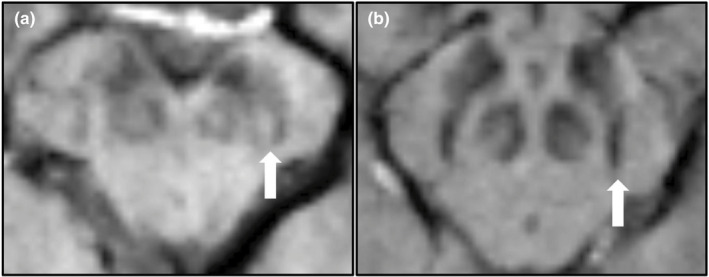
\includegraphics[width=0.8\linewidth]{FileAusiliari/Immagini/degenerative/BRB3-11-e02202-g002}
	\caption{Esempi di segno della coda di rondine (STS) in un individuo malato (a) e di STS assente in un individuo sano (b). Sono mostrate sezioni assiali del mesencefalo mappate tramite imaging pesato con suscettibilità (SWI). Le frecce bianche indicano la diversa configurazione del Nigrosoma-1 (N1). Da Brain Behav. 2021 May 24;11(7):e02202. doi: 10.1002/brb3.2202}
	\label{fig:brb3-11-e02202-g002}
\end{figure*}


La diagnosi differenziale delle sindromi parkinsoniane atipiche beneficia significativamente dell'imaging RM. L'atrofia multisistemica (MSA) evidenzia caratteristica atrofia putaminale, pontica e cerebellare, con ipointensità putaminale T2/SWI e "hot cross bun sign" pontino. La paralisi sopranucleare progressiva (PSP) manifesta atrofia mesencefalica con alterazione del rapporto mesencefalo-ponte, mentre la degenerazione corticobasale (CBD) presenta atrofia frontoparietale asimmetrica con iperintensità della sostanza bianca subcorticale.
Metodiche avanzate quali Diffusion Tensor Imaging (DTI) e risonanza magnetica funzionale (fMRI) consentono la caratterizzazione delle alterazioni microstrutturali della sostanza bianca e delle modificazioni funzionali cerebrali, sebbene la sensibilità nell'identificazione della progressione patologica e nella valutazione della risposta terapeutica necessiti ulteriore validazione. Le limitazioni metodologiche includono variabilità interindividuale e sovrapposizione dei reperti radiologici nelle diverse sindromi parkinsoniane.

\subsection{Trattamento e prognosi}

\subsection{Checklist di refertazione}

\begin{itemize}[label=$\square$] % Riquadro vuoto come simbolo
	\item Escludi altre cause di parkinsonismo (es ictus)
	\item Controlla il segnale dei nigrosomi
	\item Controlla il trofismo delle strutture sottotentoriali
\end{itemize}

\subsection{Bibliografia}
\small{
	
	
}

\note{Nota a margine}
\expl{Nota a margine colorata}
\input{Capitoli/degenerative/approccio.tex}
\input{Capitoli/degenerative/degenerative.tex}
\section{Morbo di Parkinson}

\subsection{Definizione}

\subsection{Eziologia}

\begin{figure*}[h]
	\centering
	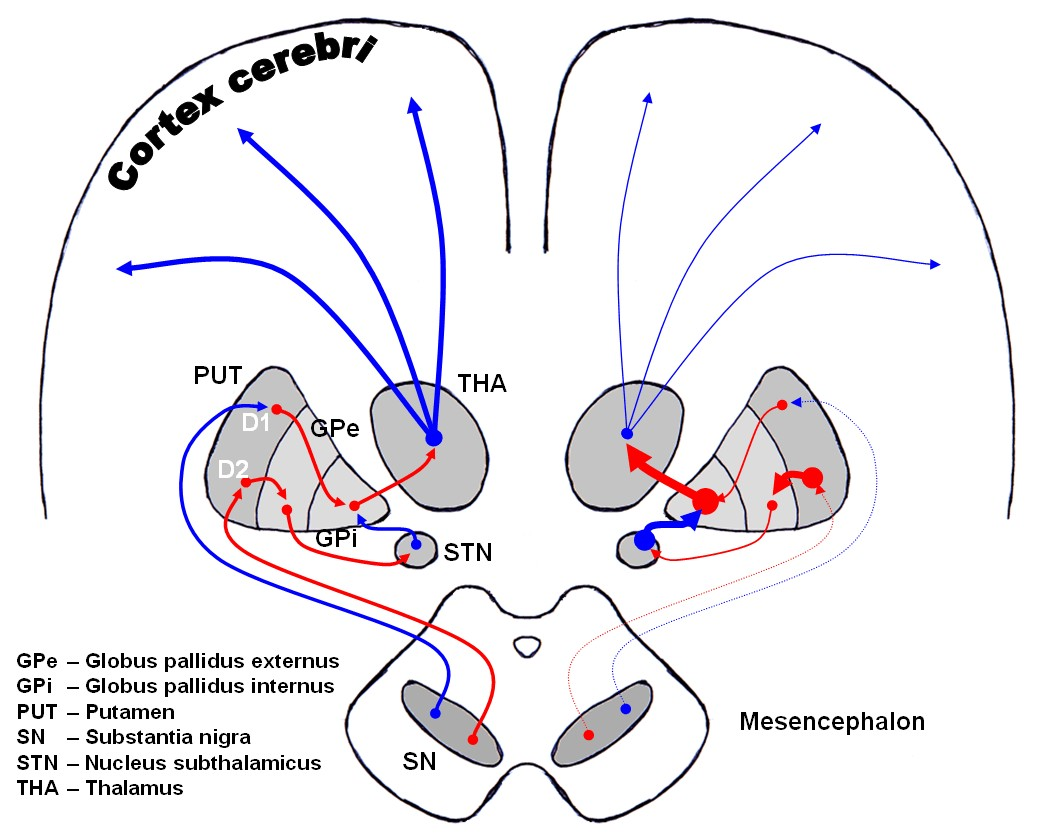
\includegraphics[width=0.5\linewidth]{FileAusiliari/Immagini/degenerative/dopamine-in-parkinsons-disease-illustration}
	\caption[Vie dopaminergiche]{L'immagine mostra le vie dopaminergiche del cervello umano in condizioni normali (a sinistra) e nella malattia di Parkinson (a destra). Le frecce rosse indicano la soppressione del bersaglio, quelle blu la stimolazione della struttura bersaglio. Caso per gentile concessione di Wikipedia, Radiopaedia.org, rID: 36286}
	\label{fig:dopamine-in-parkinsons-disease-illustration}
\end{figure*}

\subsection{Epidemiologia}
Il MP costituisce una delle principali cause di disabilità e mortalità nell'ambito delle patologie neurologiche, con una prevalenza particolarmente elevata negli Stati Uniti e in Canada (160-180 casi/100.000 abitanti). L'incidenza annuale in Nord America oscilla tra 108 e 212 casi ogni 100.000 individui di età $\geq$65 anni, con una prevalenza dello 0,3\% nella popolazione adulta $\geq$40 anni e dell'1,6\% nei soggetti ultrasessantacinquenni.
L'esordio della patologia mostra una significativa correlazione con l'età, manifestandosi tipicamente dalla quinta decade di vita, con un'età media alla diagnosi di 70,5 anni e una finestra di esordio prevalente tra i 45 e i 70 anni. Una variante giovanile può presentarsi tra i 20 e i 40 anni, sebbene l'esordio prima dei 30 anni risulti infrequente. La distribuzione per sesso evidenzia una predominanza maschile, particolarmente accentuata nella fascia d'età 50-60 anni.
L'eziologia del MP comprende fattori di rischio genetici, con particolare rilevanza nelle forme ad esordio precoce, e ambientali, tra cui l'esposizione a pesticidi e inquinanti atmosferici. Sono stati identificati fattori protettivi, inclusi il consumo di caffè, l'attività fisica e il fumo di sigaretta. La patologia si presenta prevalentemente in forma sporadica (85-90\% dei casi), mentre una minoranza dei casi (10-15\%) presenta familiarità positiva.

\subsubsection{Fattori di rischio}
L'eziopatogenesi del Morbo di Parkinson (MP) presenta una complessa interazione di fattori di rischio genetici, ambientali e non modificabili. L'anamnesi familiare positiva per MP in consanguinei di primo grado comporta un incremento del rischio relativo di 2-3 volte. Le forme monogeniche, rappresentanti meno del 10\% della casistica totale, manifestano pattern di ereditarietà autosomica dominante, recessiva o X-linked, caratterizzandosi per un esordio precoce rispetto alle forme sporadiche.
Le mutazioni eterozigoti del gene GBA1 costituiscono un significativo fattore di rischio genetico, unitamente ad alterazioni di altri geni codificanti per enzimi lisosomiali. Il coinvolgimento di geni quali SNCA, LRRK2, VPS35, Parkin, PINK1 e DJ-1 è stato ampiamente documentato. Particolare rilevanza assumono le mutazioni del gene Nurr1, determinante per l'identità neuronale dopaminergica, e del gene DJ-1, cruciale nella risposta allo stress ossidativo. Le alterazioni del gene PINK1, codificante per una chinasi mitocondriale, e del gene Park2, responsabile della sintesi della proteina parkina, sono associate a forme ad esordio precoce.
L'esposizione a neurotossine ambientali, inclusi mercurio, manganese, disolfuro di carbonio, solventi organici, MPTP e monossido di carbonio, può indurre degenerazione nigrostriatale e parkinsonismo. L'uso di neurolettici e l'abuso endovenoso di efedrone possono causare sindromi parkinsoniane potenzialmente irreversibili. Traumi cranici ripetuti, pesticidi, solventi e inquinamento atmosferico rappresentano ulteriori fattori di rischio ambientale documentati.
Tra i fattori non modificabili, l'età avanzata e il sesso maschile emergono come significativi predittori di rischio, con predominanza nella sesta decade di vita. Comorbidità quali depressione, ansia, stipsi, diabete mellito tipo 2, obesità e alterazioni del metabolismo del ferro sono state correlate a un incrementato rischio di MP.
Il consumo di tabacco e caffè, unitamente all'attività fisica regolare, ha mostrato effetti protettivi, sebbene di modesta entità. È fondamentale sottolineare che la maggioranza dei casi di MP rimane idiopatica, suggerendo un'eziologia multifattoriale.

\subsection{Presentazione  clinica}
La sintomatologia del Morbo di Parkinson manifesta un quadro clinico caratterizzato da manifestazioni motorie cardinali e sintomatologia non motoria associata. Il complesso sintomatologico motorio comprende tremore a riposo spesso asimmetrico con frequenza di 4-6 Hz, tipicamente descritto come "pill-rolling", bradicinesia manifestantesi con rallentamento motorio, ipomimia e ridotta oscillazione pendolare degli arti superiori durante la deambulazione, rigidità muscolare ("lead-pipe" o fenomeno della ruota dentata), e instabilità posturale documentabile attraverso il test della retropulsione. La deambulazione risulta caratterizzata da una progressione a piccoli passi con tendenza allo strascicamento e ridotta oscillazione degli arti superiori.
La sintomatologia accessoria include disartria con eloquio esplosivo secondario a incoordinazione linguo-diaframmatica, movimenti involontari della lingua con conseguente difficoltà protrusiva, e incremento della frequenza di ammiccamento palpebrale, quest'ultimo in contrasto con quanto osservato nella corea di Huntington. La disfunzione autonomica, i disturbi olfattivi, la sintomatologia algica, le alterazioni sensitive e i disturbi timici costituiscono il corredo sintomatologico non motorio. Il deterioramento cognitivo, con particolare coinvolgimento delle funzioni attentive, può manifestarsi e progredire nel decorso della patologia.
La progressione temporale della malattia evidenzia un esordio tipicamente unilaterale con successiva bilateralizzazione, manifestandosi prevalentemente nella sesta decade di vita. La responsività alla terapia dopaminergica, in particolare alla levodopa, rappresenta un elemento caratteristico, sebbene il tremore possa risultare farmacoresistente, in contrasto con la significativa risposta della bradicinesia e della rigidità. La variabilità fenotipica interindividuale costituisce un elemento distintivo della patologia.

\subsection{Approccio diagnostico}
L'iter diagnostico della malattia di Parkinson si fonda primariamente sulla valutazione clinica, data l'assenza di biomarcatori patognomonici. La diagnosi richiede la documentazione di bradicinesia associata ad almeno un sintomo cardine tra tremore a riposo o rigidità, valutati mediante la scala MDS-UPDRS standardizzata.
L'approccio diagnostico contempla un'accurata anamnesi ed esame obiettivo neurologico, focalizzati sull'identificazione dei sintomi cardinali: bradicinesia, tremore a riposo (4-6 Hz) tipicamente asimmetrico, rigidità e instabilità posturale. La responsività alla terapia dopaminergica, particolarmente evidente per bradicinesia e rigidità, costituisce un elemento diagnostico supportivo significativo, mentre una mancata risposta a dosaggi adeguati di levodopa suggerisce diagnosi alternative.
L'esclusione di parkinsonismi secondari richiede particolare attenzione all'insorgenza temporale dei sintomi e alla distribuzione topografica del coinvolgimento motorio. La diagnostica per immagini, sebbene non necessaria nelle presentazioni cliniche tipiche con adeguata risposta alla levodopa, può includere RM cerebrale, particolarmente utile mediante sequenze SWI per la valutazione del "swallow tail sign" nigrostriatale. La SPECT con 123I-FP-CIT (DaTscan) documenta la disfunzione dopaminergica presinaptica, mentre la PET con FDG consente la differenziazione metabolica tra PD e sindromi parkinsoniane atipiche.
L'analisi genetica, indicata in casi selezionati (esordio precoce, familiarità positiva, specifiche etnie), e la valutazione autonomica mediante scintigrafia miocardica con MIBG, che evidenzia la denervazione simpatica caratteristica, completano l'iter diagnostico. L'ecografia transcranica può evidenziare l'iperecogenicità della sostanza nera, supportando la diagnosi differenziale.
I criteri MDS stratificano la diagnosi in PD clinicamente stabilita e probabile, bilanciando specificità e sensibilità diagnostica nella pratica clinica.

\begin{Oss}
	La scala MDS-UPDRS (Movement Disorder Society-Unified Parkinson's Disease Rating Scale) è uno strumento di valutazione clinica ampiamente utilizzato per quantificare la gravità dei sintomi motori e non motori della malattia di Parkinson. Questa scala è stata sviluppata per migliorare la consistenza nella valutazione dei sintomi e per integrare meglio gli aspetti non motori della PD.
	Struttura: La scala MDS-UPDRS è composta da quattro sezioni:
	\begin{description}
		\item[Sezione I]{Esperienze non motorie della vita quotidiana. Questa sezione valuta aspetti come le capacità cognitive, i disturbi comportamentali e dell'umore}
		\item [Sezione II]{Esperienze motorie della vita quotidiana. Questa sezione valuta l'impatto dei sintomi motori sulle attività quotidiane}
		\item [Sezione III]{Esame motorio. Questa sezione valuta i segni motori della PD attraverso un esame clinico, come il tremore, la rigidità e la bradicinesia}
		\item[Sezione IV]{Complicanze della terapia. Questa sezione valuta le complicanze associate al trattamento farmacologico}
	\end{description}
	Il punteggio totale per le sezioni I-IV varia da 0 (nessuna disabilità) a 199 (disabilità totale). La sezione III, che valuta i sintomi motori, ha un punteggio che varia da 0 a 132.
	Oltre alla scala MDS-UPDRS, esistono altre scale di valutazione utilizzate nella PD, come la scala di Hoehn e Yahr e la scala di Schwab e England. La scala di Hoehn e Yahr valuta la gravità della malattia da 0 (nessuna malattia) a 5 (paziente costretto su sedia a rotelle o allettato senza assistenza).
\end{Oss}

\subsection{Anatomia patologica}
Dal punto di vista anatomopatologico il morbo di Parkinson si manifesta attraverso inclusioni proteiche intraneuronali denominate corpi di Lewy, costituiti primariamente da aggregati patologici di alfa-sinucleina, una proteina sinaptica fisiologicamente presente nel sistema nervoso centrale. L'accumulo di queste inclusioni, sebbene non patognomonico del morbo di Parkinson essendo documentabile anche nella demenza a corpi di Lewy, rappresenta una caratteristica istopatologica fondamentale quando localizzato nella substantia nigra, in associazione alla perdita neuronale dopaminergica. L'assenza di corpi di Lewy nelle forme post-encefalitiche, caratterizzate invece da grovigli neurofibrillari, e in alcune forme geneticamente determinate, sottolinea l'eterogeneità patogenetica della malattia.
La progressione spazio-temporale della patologia, codificata nello staging di Braak, delinea sei stadi evolutivi caratterizzati da una diffusione ascendente delle alterazioni neuropatologiche. Gli stadi iniziali (1-2) coinvolgono il nucleo motore dorsale dei nervi glossofaringeo e vago e il nucleo olfattivo anteriore, precedendo frequentemente la sintomatologia motoria. Gli stadi intermedi (3-4) documentano il coinvolgimento della substantia nigra pars compacta, del prosencefalo basale e della mesocorteccia temporale, correlando con l'esordio clinico della malattia. Gli stadi terminali (5-6) evidenziano una progressione neocorticale diffusa.
La patogenesi molecolare implica alterazioni del metabolismo dell'alfa-sinucleina, potenzialmente accelerate da disfunzioni delle proteine heat shock o dall'azione della dopamina. Il coinvolgimento della proteina parkin nella degradazione proteasomica evidenzia meccanismi neurodegenerativi potenzialmente indipendenti dalla formazione dei corpi di Lewy.
L'alfa-sinucleina, proteina fisiologicamente localizzata nelle terminazioni presinaptiche neuronali, manifesta nella patogenesi del morbo di Parkinson un processo patologico caratterizzato da misfolding proteico e successiva aggregazione in oligomeri, protofibrille e fibrille, culminante nella formazione dei corpi di Lewy intraneuronali. Questi aggregati proteici, considerati hallmark istopatologico della malattia, evidenziano particolare neurotossicità nella forma protofibrillare, determinando disfunzione e successiva degenerazione neuronale dopaminergica nigrostriatale.
L'identificazione di mutazioni nel gene SNCA, codificante per l'alfa-sinucleina, nelle forme familiari di malattia, unitamente alla documentazione di fenotipi clinici particolarmente aggressivi in presenza di duplicazione o triplicazione genica, ha fornito evidenze significative del ruolo causale di questa proteina nella patogenesi della malattia. La documentata capacità di trasmissione transcellulare dell'alfa-sinucleina patologica costituisce il substrato molecolare della progressione anatomopatologica descritta nello staging di Braak.
La disfunzione sinaptica correlata all'accumulo di alfa-sinucleina rappresenta un meccanismo patogenetico critico, modulato da fattori quali stress ossidativo, alterazioni del sistema ubiquitina-proteasoma e interazione con il metabolismo dopaminergico. Mutazioni nei geni parkin, PINK1 e DJ-1 influenzano il metabolismo dell'alfa-sinucleina attraverso alterazioni dei sistemi di degradazione proteica.
L'alfa-sinucleina costituisce attualmente un promettente target terapeutico, con particolare interesse per lo sviluppo di anticorpi monoclonali specifici e inibitori dell'aggregazione proteica, finalizzati al rallentamento della progressione patologica.

\subsection{Imaging}

\subsubsection{TC}
La TC manifesta un'utilità clinica circoscritta nella valutazione diagnostica primaria del MP, assumendo rilevanza nell'esclusione di patologie strutturali mimiche quali lesioni espansive, idrocefalo o alterazioni vascolari, particolarmente in presenza di presentazioni cliniche atipiche o "red flags" suggestive di diagnosi alternative.
Nel contesto della gestione terapeutica, la TC assume particolare rilevanza nella valutazione post-chirurgica della stimolazione cerebrale profonda (DBS), consentendo la verifica del corretto posizionamento degli elettrodi nel nucleo subtalamico (STN), tipicamente localizzati a 9mm dalla linea mediana, e l'identificazione di eventuali complicanze post-procedurali quali eventi emorragici, ischemici o fenomeni infiammatori transitori, questi ultimi caratterizzati da aree ipodense perilettrodiche a risoluzione graduale. L'utilità della metodica nel follow-up routinario post-DBS risulta secondaria.
La sensibilità subottimale della TC nella diagnosi differenziale tra PD e sindromi parkinsoniane atipiche, incluse atrofia multisistemica e paralisi sopranucleare progressiva, nonché nella distinzione dal tremore essenziale, ne limita significativamente l'applicazione clinica in questo contesto diagnostico.

\subsubsection{RM}
La RM è frequentemente normale nelle sequenze convenzionali (T1, T2, FLAIR) nelle fasi iniziali di malattia. L'implementazione di sequenze susceptibility-weighted imaging (SWI) o T2*-weighted ad alta risoluzione consente la visualizzazione del nigrosoma-1, struttura caratterizzata dal patognomonico "swallow tail sign", la cui perdita correla con la degenerazione dopaminergica nigrostriatale. L'accumulo patologico di ferro nella substantia nigra, quantificabile mediante sequenze SWI/T2* e incrementato del 50\% rispetto ai controlli, costituisce un ulteriore marker diagnostico, complementato dall'imaging della neuromelanina mediante sequenze T1 con impulsi di trasferimento di magnetizzazione (MTC).

\begin{figure*}[h]
	\centering
	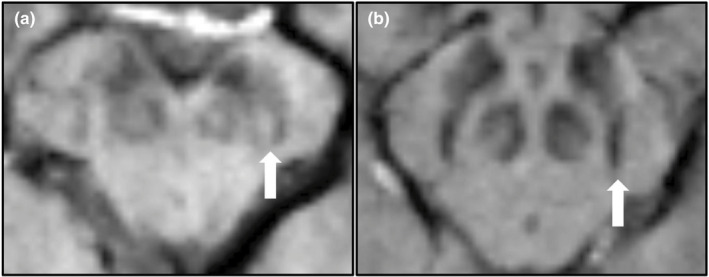
\includegraphics[width=0.8\linewidth]{FileAusiliari/Immagini/degenerative/BRB3-11-e02202-g002}
	\caption{Esempi di segno della coda di rondine (STS) in un individuo malato (a) e di STS assente in un individuo sano (b). Sono mostrate sezioni assiali del mesencefalo mappate tramite imaging pesato con suscettibilità (SWI). Le frecce bianche indicano la diversa configurazione del Nigrosoma-1 (N1). Da Brain Behav. 2021 May 24;11(7):e02202. doi: 10.1002/brb3.2202}
	\label{fig:brb3-11-e02202-g002}
\end{figure*}


La diagnosi differenziale delle sindromi parkinsoniane atipiche beneficia significativamente dell'imaging RM. L'atrofia multisistemica (MSA) evidenzia caratteristica atrofia putaminale, pontica e cerebellare, con ipointensità putaminale T2/SWI e "hot cross bun sign" pontino. La paralisi sopranucleare progressiva (PSP) manifesta atrofia mesencefalica con alterazione del rapporto mesencefalo-ponte, mentre la degenerazione corticobasale (CBD) presenta atrofia frontoparietale asimmetrica con iperintensità della sostanza bianca subcorticale.
Metodiche avanzate quali Diffusion Tensor Imaging (DTI) e risonanza magnetica funzionale (fMRI) consentono la caratterizzazione delle alterazioni microstrutturali della sostanza bianca e delle modificazioni funzionali cerebrali, sebbene la sensibilità nell'identificazione della progressione patologica e nella valutazione della risposta terapeutica necessiti ulteriore validazione. Le limitazioni metodologiche includono variabilità interindividuale e sovrapposizione dei reperti radiologici nelle diverse sindromi parkinsoniane.

\subsection{Trattamento e prognosi}

\subsection{Checklist di refertazione}

\begin{itemize}[label=$\square$] % Riquadro vuoto come simbolo
	\item Escludi altre cause di parkinsonismo (es ictus)
	\item Controlla il segnale dei nigrosomi
	\item Controlla il trofismo delle strutture sottotentoriali
\end{itemize}

\subsection{Bibliografia}
\small{
	
	
}

\note{Nota a margine}
\expl{Nota a margine colorata}
\input{Capitoli/degenerative/approccio.tex}
\input{Capitoli/degenerative/degenerative.tex}
\section{Morbo di Parkinson}

\subsection{Definizione}

\subsection{Eziologia}

\begin{figure*}[h]
	\centering
	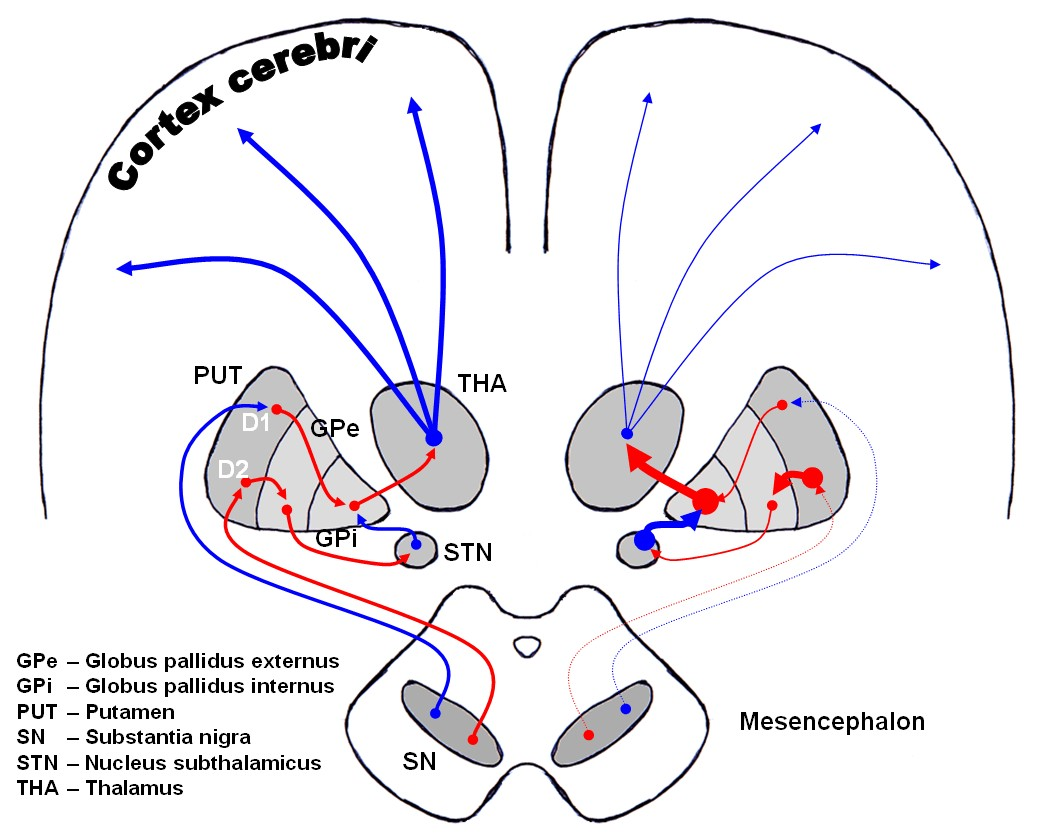
\includegraphics[width=0.5\linewidth]{FileAusiliari/Immagini/degenerative/dopamine-in-parkinsons-disease-illustration}
	\caption[Vie dopaminergiche]{L'immagine mostra le vie dopaminergiche del cervello umano in condizioni normali (a sinistra) e nella malattia di Parkinson (a destra). Le frecce rosse indicano la soppressione del bersaglio, quelle blu la stimolazione della struttura bersaglio. Caso per gentile concessione di Wikipedia, Radiopaedia.org, rID: 36286}
	\label{fig:dopamine-in-parkinsons-disease-illustration}
\end{figure*}

\subsection{Epidemiologia}
Il MP costituisce una delle principali cause di disabilità e mortalità nell'ambito delle patologie neurologiche, con una prevalenza particolarmente elevata negli Stati Uniti e in Canada (160-180 casi/100.000 abitanti). L'incidenza annuale in Nord America oscilla tra 108 e 212 casi ogni 100.000 individui di età $\geq$65 anni, con una prevalenza dello 0,3\% nella popolazione adulta $\geq$40 anni e dell'1,6\% nei soggetti ultrasessantacinquenni.
L'esordio della patologia mostra una significativa correlazione con l'età, manifestandosi tipicamente dalla quinta decade di vita, con un'età media alla diagnosi di 70,5 anni e una finestra di esordio prevalente tra i 45 e i 70 anni. Una variante giovanile può presentarsi tra i 20 e i 40 anni, sebbene l'esordio prima dei 30 anni risulti infrequente. La distribuzione per sesso evidenzia una predominanza maschile, particolarmente accentuata nella fascia d'età 50-60 anni.
L'eziologia del MP comprende fattori di rischio genetici, con particolare rilevanza nelle forme ad esordio precoce, e ambientali, tra cui l'esposizione a pesticidi e inquinanti atmosferici. Sono stati identificati fattori protettivi, inclusi il consumo di caffè, l'attività fisica e il fumo di sigaretta. La patologia si presenta prevalentemente in forma sporadica (85-90\% dei casi), mentre una minoranza dei casi (10-15\%) presenta familiarità positiva.

\subsubsection{Fattori di rischio}
L'eziopatogenesi del Morbo di Parkinson (MP) presenta una complessa interazione di fattori di rischio genetici, ambientali e non modificabili. L'anamnesi familiare positiva per MP in consanguinei di primo grado comporta un incremento del rischio relativo di 2-3 volte. Le forme monogeniche, rappresentanti meno del 10\% della casistica totale, manifestano pattern di ereditarietà autosomica dominante, recessiva o X-linked, caratterizzandosi per un esordio precoce rispetto alle forme sporadiche.
Le mutazioni eterozigoti del gene GBA1 costituiscono un significativo fattore di rischio genetico, unitamente ad alterazioni di altri geni codificanti per enzimi lisosomiali. Il coinvolgimento di geni quali SNCA, LRRK2, VPS35, Parkin, PINK1 e DJ-1 è stato ampiamente documentato. Particolare rilevanza assumono le mutazioni del gene Nurr1, determinante per l'identità neuronale dopaminergica, e del gene DJ-1, cruciale nella risposta allo stress ossidativo. Le alterazioni del gene PINK1, codificante per una chinasi mitocondriale, e del gene Park2, responsabile della sintesi della proteina parkina, sono associate a forme ad esordio precoce.
L'esposizione a neurotossine ambientali, inclusi mercurio, manganese, disolfuro di carbonio, solventi organici, MPTP e monossido di carbonio, può indurre degenerazione nigrostriatale e parkinsonismo. L'uso di neurolettici e l'abuso endovenoso di efedrone possono causare sindromi parkinsoniane potenzialmente irreversibili. Traumi cranici ripetuti, pesticidi, solventi e inquinamento atmosferico rappresentano ulteriori fattori di rischio ambientale documentati.
Tra i fattori non modificabili, l'età avanzata e il sesso maschile emergono come significativi predittori di rischio, con predominanza nella sesta decade di vita. Comorbidità quali depressione, ansia, stipsi, diabete mellito tipo 2, obesità e alterazioni del metabolismo del ferro sono state correlate a un incrementato rischio di MP.
Il consumo di tabacco e caffè, unitamente all'attività fisica regolare, ha mostrato effetti protettivi, sebbene di modesta entità. È fondamentale sottolineare che la maggioranza dei casi di MP rimane idiopatica, suggerendo un'eziologia multifattoriale.

\subsection{Presentazione  clinica}
La sintomatologia del Morbo di Parkinson manifesta un quadro clinico caratterizzato da manifestazioni motorie cardinali e sintomatologia non motoria associata. Il complesso sintomatologico motorio comprende tremore a riposo spesso asimmetrico con frequenza di 4-6 Hz, tipicamente descritto come "pill-rolling", bradicinesia manifestantesi con rallentamento motorio, ipomimia e ridotta oscillazione pendolare degli arti superiori durante la deambulazione, rigidità muscolare ("lead-pipe" o fenomeno della ruota dentata), e instabilità posturale documentabile attraverso il test della retropulsione. La deambulazione risulta caratterizzata da una progressione a piccoli passi con tendenza allo strascicamento e ridotta oscillazione degli arti superiori.
La sintomatologia accessoria include disartria con eloquio esplosivo secondario a incoordinazione linguo-diaframmatica, movimenti involontari della lingua con conseguente difficoltà protrusiva, e incremento della frequenza di ammiccamento palpebrale, quest'ultimo in contrasto con quanto osservato nella corea di Huntington. La disfunzione autonomica, i disturbi olfattivi, la sintomatologia algica, le alterazioni sensitive e i disturbi timici costituiscono il corredo sintomatologico non motorio. Il deterioramento cognitivo, con particolare coinvolgimento delle funzioni attentive, può manifestarsi e progredire nel decorso della patologia.
La progressione temporale della malattia evidenzia un esordio tipicamente unilaterale con successiva bilateralizzazione, manifestandosi prevalentemente nella sesta decade di vita. La responsività alla terapia dopaminergica, in particolare alla levodopa, rappresenta un elemento caratteristico, sebbene il tremore possa risultare farmacoresistente, in contrasto con la significativa risposta della bradicinesia e della rigidità. La variabilità fenotipica interindividuale costituisce un elemento distintivo della patologia.

\subsection{Approccio diagnostico}
L'iter diagnostico della malattia di Parkinson si fonda primariamente sulla valutazione clinica, data l'assenza di biomarcatori patognomonici. La diagnosi richiede la documentazione di bradicinesia associata ad almeno un sintomo cardine tra tremore a riposo o rigidità, valutati mediante la scala MDS-UPDRS standardizzata.
L'approccio diagnostico contempla un'accurata anamnesi ed esame obiettivo neurologico, focalizzati sull'identificazione dei sintomi cardinali: bradicinesia, tremore a riposo (4-6 Hz) tipicamente asimmetrico, rigidità e instabilità posturale. La responsività alla terapia dopaminergica, particolarmente evidente per bradicinesia e rigidità, costituisce un elemento diagnostico supportivo significativo, mentre una mancata risposta a dosaggi adeguati di levodopa suggerisce diagnosi alternative.
L'esclusione di parkinsonismi secondari richiede particolare attenzione all'insorgenza temporale dei sintomi e alla distribuzione topografica del coinvolgimento motorio. La diagnostica per immagini, sebbene non necessaria nelle presentazioni cliniche tipiche con adeguata risposta alla levodopa, può includere RM cerebrale, particolarmente utile mediante sequenze SWI per la valutazione del "swallow tail sign" nigrostriatale. La SPECT con 123I-FP-CIT (DaTscan) documenta la disfunzione dopaminergica presinaptica, mentre la PET con FDG consente la differenziazione metabolica tra PD e sindromi parkinsoniane atipiche.
L'analisi genetica, indicata in casi selezionati (esordio precoce, familiarità positiva, specifiche etnie), e la valutazione autonomica mediante scintigrafia miocardica con MIBG, che evidenzia la denervazione simpatica caratteristica, completano l'iter diagnostico. L'ecografia transcranica può evidenziare l'iperecogenicità della sostanza nera, supportando la diagnosi differenziale.
I criteri MDS stratificano la diagnosi in PD clinicamente stabilita e probabile, bilanciando specificità e sensibilità diagnostica nella pratica clinica.

\begin{Oss}
	La scala MDS-UPDRS (Movement Disorder Society-Unified Parkinson's Disease Rating Scale) è uno strumento di valutazione clinica ampiamente utilizzato per quantificare la gravità dei sintomi motori e non motori della malattia di Parkinson. Questa scala è stata sviluppata per migliorare la consistenza nella valutazione dei sintomi e per integrare meglio gli aspetti non motori della PD.
	Struttura: La scala MDS-UPDRS è composta da quattro sezioni:
	\begin{description}
		\item[Sezione I]{Esperienze non motorie della vita quotidiana. Questa sezione valuta aspetti come le capacità cognitive, i disturbi comportamentali e dell'umore}
		\item [Sezione II]{Esperienze motorie della vita quotidiana. Questa sezione valuta l'impatto dei sintomi motori sulle attività quotidiane}
		\item [Sezione III]{Esame motorio. Questa sezione valuta i segni motori della PD attraverso un esame clinico, come il tremore, la rigidità e la bradicinesia}
		\item[Sezione IV]{Complicanze della terapia. Questa sezione valuta le complicanze associate al trattamento farmacologico}
	\end{description}
	Il punteggio totale per le sezioni I-IV varia da 0 (nessuna disabilità) a 199 (disabilità totale). La sezione III, che valuta i sintomi motori, ha un punteggio che varia da 0 a 132.
	Oltre alla scala MDS-UPDRS, esistono altre scale di valutazione utilizzate nella PD, come la scala di Hoehn e Yahr e la scala di Schwab e England. La scala di Hoehn e Yahr valuta la gravità della malattia da 0 (nessuna malattia) a 5 (paziente costretto su sedia a rotelle o allettato senza assistenza).
\end{Oss}

\subsection{Anatomia patologica}
Dal punto di vista anatomopatologico il morbo di Parkinson si manifesta attraverso inclusioni proteiche intraneuronali denominate corpi di Lewy, costituiti primariamente da aggregati patologici di alfa-sinucleina, una proteina sinaptica fisiologicamente presente nel sistema nervoso centrale. L'accumulo di queste inclusioni, sebbene non patognomonico del morbo di Parkinson essendo documentabile anche nella demenza a corpi di Lewy, rappresenta una caratteristica istopatologica fondamentale quando localizzato nella substantia nigra, in associazione alla perdita neuronale dopaminergica. L'assenza di corpi di Lewy nelle forme post-encefalitiche, caratterizzate invece da grovigli neurofibrillari, e in alcune forme geneticamente determinate, sottolinea l'eterogeneità patogenetica della malattia.
La progressione spazio-temporale della patologia, codificata nello staging di Braak, delinea sei stadi evolutivi caratterizzati da una diffusione ascendente delle alterazioni neuropatologiche. Gli stadi iniziali (1-2) coinvolgono il nucleo motore dorsale dei nervi glossofaringeo e vago e il nucleo olfattivo anteriore, precedendo frequentemente la sintomatologia motoria. Gli stadi intermedi (3-4) documentano il coinvolgimento della substantia nigra pars compacta, del prosencefalo basale e della mesocorteccia temporale, correlando con l'esordio clinico della malattia. Gli stadi terminali (5-6) evidenziano una progressione neocorticale diffusa.
La patogenesi molecolare implica alterazioni del metabolismo dell'alfa-sinucleina, potenzialmente accelerate da disfunzioni delle proteine heat shock o dall'azione della dopamina. Il coinvolgimento della proteina parkin nella degradazione proteasomica evidenzia meccanismi neurodegenerativi potenzialmente indipendenti dalla formazione dei corpi di Lewy.
L'alfa-sinucleina, proteina fisiologicamente localizzata nelle terminazioni presinaptiche neuronali, manifesta nella patogenesi del morbo di Parkinson un processo patologico caratterizzato da misfolding proteico e successiva aggregazione in oligomeri, protofibrille e fibrille, culminante nella formazione dei corpi di Lewy intraneuronali. Questi aggregati proteici, considerati hallmark istopatologico della malattia, evidenziano particolare neurotossicità nella forma protofibrillare, determinando disfunzione e successiva degenerazione neuronale dopaminergica nigrostriatale.
L'identificazione di mutazioni nel gene SNCA, codificante per l'alfa-sinucleina, nelle forme familiari di malattia, unitamente alla documentazione di fenotipi clinici particolarmente aggressivi in presenza di duplicazione o triplicazione genica, ha fornito evidenze significative del ruolo causale di questa proteina nella patogenesi della malattia. La documentata capacità di trasmissione transcellulare dell'alfa-sinucleina patologica costituisce il substrato molecolare della progressione anatomopatologica descritta nello staging di Braak.
La disfunzione sinaptica correlata all'accumulo di alfa-sinucleina rappresenta un meccanismo patogenetico critico, modulato da fattori quali stress ossidativo, alterazioni del sistema ubiquitina-proteasoma e interazione con il metabolismo dopaminergico. Mutazioni nei geni parkin, PINK1 e DJ-1 influenzano il metabolismo dell'alfa-sinucleina attraverso alterazioni dei sistemi di degradazione proteica.
L'alfa-sinucleina costituisce attualmente un promettente target terapeutico, con particolare interesse per lo sviluppo di anticorpi monoclonali specifici e inibitori dell'aggregazione proteica, finalizzati al rallentamento della progressione patologica.

\subsection{Imaging}

\subsubsection{TC}
La TC manifesta un'utilità clinica circoscritta nella valutazione diagnostica primaria del MP, assumendo rilevanza nell'esclusione di patologie strutturali mimiche quali lesioni espansive, idrocefalo o alterazioni vascolari, particolarmente in presenza di presentazioni cliniche atipiche o "red flags" suggestive di diagnosi alternative.
Nel contesto della gestione terapeutica, la TC assume particolare rilevanza nella valutazione post-chirurgica della stimolazione cerebrale profonda (DBS), consentendo la verifica del corretto posizionamento degli elettrodi nel nucleo subtalamico (STN), tipicamente localizzati a 9mm dalla linea mediana, e l'identificazione di eventuali complicanze post-procedurali quali eventi emorragici, ischemici o fenomeni infiammatori transitori, questi ultimi caratterizzati da aree ipodense perilettrodiche a risoluzione graduale. L'utilità della metodica nel follow-up routinario post-DBS risulta secondaria.
La sensibilità subottimale della TC nella diagnosi differenziale tra PD e sindromi parkinsoniane atipiche, incluse atrofia multisistemica e paralisi sopranucleare progressiva, nonché nella distinzione dal tremore essenziale, ne limita significativamente l'applicazione clinica in questo contesto diagnostico.

\subsubsection{RM}
La RM è frequentemente normale nelle sequenze convenzionali (T1, T2, FLAIR) nelle fasi iniziali di malattia. L'implementazione di sequenze susceptibility-weighted imaging (SWI) o T2*-weighted ad alta risoluzione consente la visualizzazione del nigrosoma-1, struttura caratterizzata dal patognomonico "swallow tail sign", la cui perdita correla con la degenerazione dopaminergica nigrostriatale. L'accumulo patologico di ferro nella substantia nigra, quantificabile mediante sequenze SWI/T2* e incrementato del 50\% rispetto ai controlli, costituisce un ulteriore marker diagnostico, complementato dall'imaging della neuromelanina mediante sequenze T1 con impulsi di trasferimento di magnetizzazione (MTC).

\begin{figure*}[h]
	\centering
	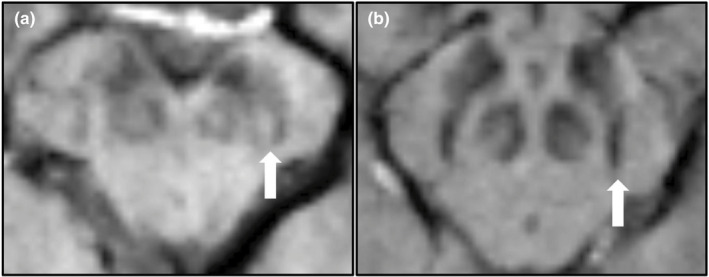
\includegraphics[width=0.8\linewidth]{FileAusiliari/Immagini/degenerative/BRB3-11-e02202-g002}
	\caption{Esempi di segno della coda di rondine (STS) in un individuo malato (a) e di STS assente in un individuo sano (b). Sono mostrate sezioni assiali del mesencefalo mappate tramite imaging pesato con suscettibilità (SWI). Le frecce bianche indicano la diversa configurazione del Nigrosoma-1 (N1). Da Brain Behav. 2021 May 24;11(7):e02202. doi: 10.1002/brb3.2202}
	\label{fig:brb3-11-e02202-g002}
\end{figure*}


La diagnosi differenziale delle sindromi parkinsoniane atipiche beneficia significativamente dell'imaging RM. L'atrofia multisistemica (MSA) evidenzia caratteristica atrofia putaminale, pontica e cerebellare, con ipointensità putaminale T2/SWI e "hot cross bun sign" pontino. La paralisi sopranucleare progressiva (PSP) manifesta atrofia mesencefalica con alterazione del rapporto mesencefalo-ponte, mentre la degenerazione corticobasale (CBD) presenta atrofia frontoparietale asimmetrica con iperintensità della sostanza bianca subcorticale.
Metodiche avanzate quali Diffusion Tensor Imaging (DTI) e risonanza magnetica funzionale (fMRI) consentono la caratterizzazione delle alterazioni microstrutturali della sostanza bianca e delle modificazioni funzionali cerebrali, sebbene la sensibilità nell'identificazione della progressione patologica e nella valutazione della risposta terapeutica necessiti ulteriore validazione. Le limitazioni metodologiche includono variabilità interindividuale e sovrapposizione dei reperti radiologici nelle diverse sindromi parkinsoniane.

\subsection{Trattamento e prognosi}

\subsection{Checklist di refertazione}

\begin{itemize}[label=$\square$] % Riquadro vuoto come simbolo
	\item Escludi altre cause di parkinsonismo (es ictus)
	\item Controlla il segnale dei nigrosomi
	\item Controlla il trofismo delle strutture sottotentoriali
\end{itemize}

\subsection{Bibliografia}
\small{
	
	
}

\note{Nota a margine}
\expl{Nota a margine colorata}
\input{Capitoli/degenerative/approccio.tex}
\input{Capitoli/degenerative/degenerative.tex}
\section{Morbo di Parkinson}

\subsection{Definizione}

\subsection{Eziologia}

\begin{figure*}[h]
	\centering
	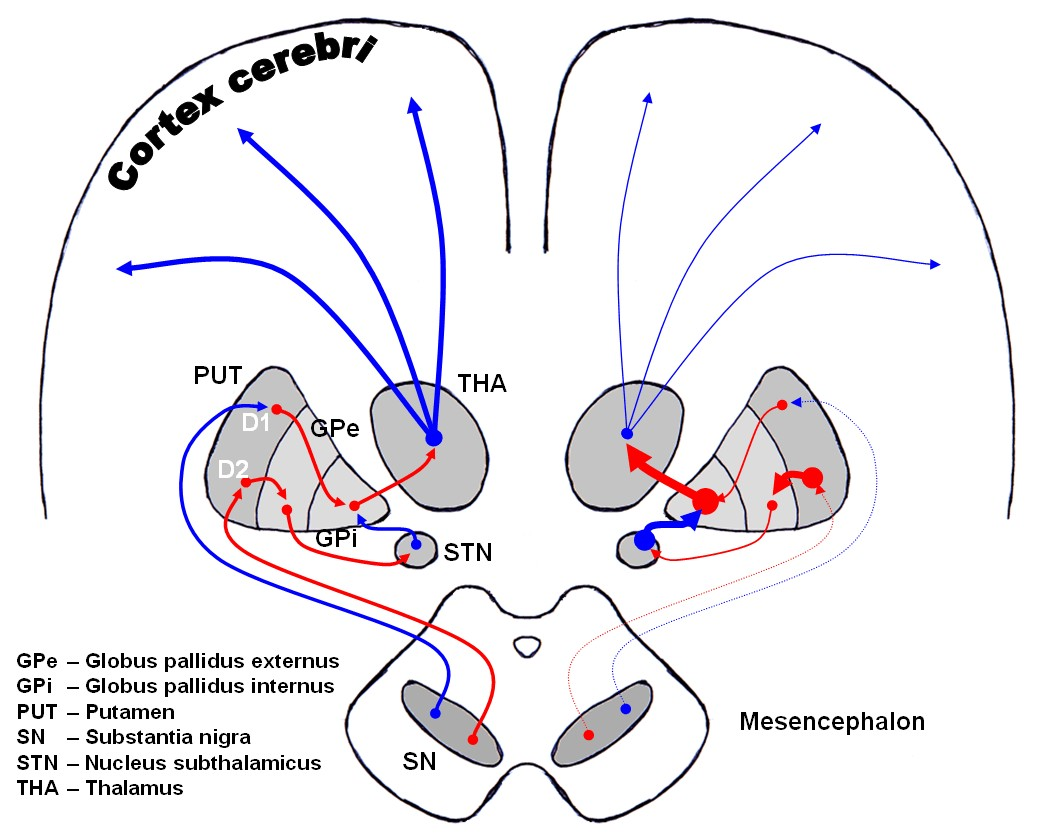
\includegraphics[width=0.5\linewidth]{FileAusiliari/Immagini/degenerative/dopamine-in-parkinsons-disease-illustration}
	\caption[Vie dopaminergiche]{L'immagine mostra le vie dopaminergiche del cervello umano in condizioni normali (a sinistra) e nella malattia di Parkinson (a destra). Le frecce rosse indicano la soppressione del bersaglio, quelle blu la stimolazione della struttura bersaglio. Caso per gentile concessione di Wikipedia, Radiopaedia.org, rID: 36286}
	\label{fig:dopamine-in-parkinsons-disease-illustration}
\end{figure*}

\subsection{Epidemiologia}
Il MP costituisce una delle principali cause di disabilità e mortalità nell'ambito delle patologie neurologiche, con una prevalenza particolarmente elevata negli Stati Uniti e in Canada (160-180 casi/100.000 abitanti). L'incidenza annuale in Nord America oscilla tra 108 e 212 casi ogni 100.000 individui di età $\geq$65 anni, con una prevalenza dello 0,3\% nella popolazione adulta $\geq$40 anni e dell'1,6\% nei soggetti ultrasessantacinquenni.
L'esordio della patologia mostra una significativa correlazione con l'età, manifestandosi tipicamente dalla quinta decade di vita, con un'età media alla diagnosi di 70,5 anni e una finestra di esordio prevalente tra i 45 e i 70 anni. Una variante giovanile può presentarsi tra i 20 e i 40 anni, sebbene l'esordio prima dei 30 anni risulti infrequente. La distribuzione per sesso evidenzia una predominanza maschile, particolarmente accentuata nella fascia d'età 50-60 anni.
L'eziologia del MP comprende fattori di rischio genetici, con particolare rilevanza nelle forme ad esordio precoce, e ambientali, tra cui l'esposizione a pesticidi e inquinanti atmosferici. Sono stati identificati fattori protettivi, inclusi il consumo di caffè, l'attività fisica e il fumo di sigaretta. La patologia si presenta prevalentemente in forma sporadica (85-90\% dei casi), mentre una minoranza dei casi (10-15\%) presenta familiarità positiva.

\subsubsection{Fattori di rischio}
L'eziopatogenesi del Morbo di Parkinson (MP) presenta una complessa interazione di fattori di rischio genetici, ambientali e non modificabili. L'anamnesi familiare positiva per MP in consanguinei di primo grado comporta un incremento del rischio relativo di 2-3 volte. Le forme monogeniche, rappresentanti meno del 10\% della casistica totale, manifestano pattern di ereditarietà autosomica dominante, recessiva o X-linked, caratterizzandosi per un esordio precoce rispetto alle forme sporadiche.
Le mutazioni eterozigoti del gene GBA1 costituiscono un significativo fattore di rischio genetico, unitamente ad alterazioni di altri geni codificanti per enzimi lisosomiali. Il coinvolgimento di geni quali SNCA, LRRK2, VPS35, Parkin, PINK1 e DJ-1 è stato ampiamente documentato. Particolare rilevanza assumono le mutazioni del gene Nurr1, determinante per l'identità neuronale dopaminergica, e del gene DJ-1, cruciale nella risposta allo stress ossidativo. Le alterazioni del gene PINK1, codificante per una chinasi mitocondriale, e del gene Park2, responsabile della sintesi della proteina parkina, sono associate a forme ad esordio precoce.
L'esposizione a neurotossine ambientali, inclusi mercurio, manganese, disolfuro di carbonio, solventi organici, MPTP e monossido di carbonio, può indurre degenerazione nigrostriatale e parkinsonismo. L'uso di neurolettici e l'abuso endovenoso di efedrone possono causare sindromi parkinsoniane potenzialmente irreversibili. Traumi cranici ripetuti, pesticidi, solventi e inquinamento atmosferico rappresentano ulteriori fattori di rischio ambientale documentati.
Tra i fattori non modificabili, l'età avanzata e il sesso maschile emergono come significativi predittori di rischio, con predominanza nella sesta decade di vita. Comorbidità quali depressione, ansia, stipsi, diabete mellito tipo 2, obesità e alterazioni del metabolismo del ferro sono state correlate a un incrementato rischio di MP.
Il consumo di tabacco e caffè, unitamente all'attività fisica regolare, ha mostrato effetti protettivi, sebbene di modesta entità. È fondamentale sottolineare che la maggioranza dei casi di MP rimane idiopatica, suggerendo un'eziologia multifattoriale.

\subsection{Presentazione  clinica}
La sintomatologia del Morbo di Parkinson manifesta un quadro clinico caratterizzato da manifestazioni motorie cardinali e sintomatologia non motoria associata. Il complesso sintomatologico motorio comprende tremore a riposo spesso asimmetrico con frequenza di 4-6 Hz, tipicamente descritto come "pill-rolling", bradicinesia manifestantesi con rallentamento motorio, ipomimia e ridotta oscillazione pendolare degli arti superiori durante la deambulazione, rigidità muscolare ("lead-pipe" o fenomeno della ruota dentata), e instabilità posturale documentabile attraverso il test della retropulsione. La deambulazione risulta caratterizzata da una progressione a piccoli passi con tendenza allo strascicamento e ridotta oscillazione degli arti superiori.
La sintomatologia accessoria include disartria con eloquio esplosivo secondario a incoordinazione linguo-diaframmatica, movimenti involontari della lingua con conseguente difficoltà protrusiva, e incremento della frequenza di ammiccamento palpebrale, quest'ultimo in contrasto con quanto osservato nella corea di Huntington. La disfunzione autonomica, i disturbi olfattivi, la sintomatologia algica, le alterazioni sensitive e i disturbi timici costituiscono il corredo sintomatologico non motorio. Il deterioramento cognitivo, con particolare coinvolgimento delle funzioni attentive, può manifestarsi e progredire nel decorso della patologia.
La progressione temporale della malattia evidenzia un esordio tipicamente unilaterale con successiva bilateralizzazione, manifestandosi prevalentemente nella sesta decade di vita. La responsività alla terapia dopaminergica, in particolare alla levodopa, rappresenta un elemento caratteristico, sebbene il tremore possa risultare farmacoresistente, in contrasto con la significativa risposta della bradicinesia e della rigidità. La variabilità fenotipica interindividuale costituisce un elemento distintivo della patologia.

\subsection{Approccio diagnostico}
L'iter diagnostico della malattia di Parkinson si fonda primariamente sulla valutazione clinica, data l'assenza di biomarcatori patognomonici. La diagnosi richiede la documentazione di bradicinesia associata ad almeno un sintomo cardine tra tremore a riposo o rigidità, valutati mediante la scala MDS-UPDRS standardizzata.
L'approccio diagnostico contempla un'accurata anamnesi ed esame obiettivo neurologico, focalizzati sull'identificazione dei sintomi cardinali: bradicinesia, tremore a riposo (4-6 Hz) tipicamente asimmetrico, rigidità e instabilità posturale. La responsività alla terapia dopaminergica, particolarmente evidente per bradicinesia e rigidità, costituisce un elemento diagnostico supportivo significativo, mentre una mancata risposta a dosaggi adeguati di levodopa suggerisce diagnosi alternative.
L'esclusione di parkinsonismi secondari richiede particolare attenzione all'insorgenza temporale dei sintomi e alla distribuzione topografica del coinvolgimento motorio. La diagnostica per immagini, sebbene non necessaria nelle presentazioni cliniche tipiche con adeguata risposta alla levodopa, può includere RM cerebrale, particolarmente utile mediante sequenze SWI per la valutazione del "swallow tail sign" nigrostriatale. La SPECT con 123I-FP-CIT (DaTscan) documenta la disfunzione dopaminergica presinaptica, mentre la PET con FDG consente la differenziazione metabolica tra PD e sindromi parkinsoniane atipiche.
L'analisi genetica, indicata in casi selezionati (esordio precoce, familiarità positiva, specifiche etnie), e la valutazione autonomica mediante scintigrafia miocardica con MIBG, che evidenzia la denervazione simpatica caratteristica, completano l'iter diagnostico. L'ecografia transcranica può evidenziare l'iperecogenicità della sostanza nera, supportando la diagnosi differenziale.
I criteri MDS stratificano la diagnosi in PD clinicamente stabilita e probabile, bilanciando specificità e sensibilità diagnostica nella pratica clinica.

\begin{Oss}
	La scala MDS-UPDRS (Movement Disorder Society-Unified Parkinson's Disease Rating Scale) è uno strumento di valutazione clinica ampiamente utilizzato per quantificare la gravità dei sintomi motori e non motori della malattia di Parkinson. Questa scala è stata sviluppata per migliorare la consistenza nella valutazione dei sintomi e per integrare meglio gli aspetti non motori della PD.
	Struttura: La scala MDS-UPDRS è composta da quattro sezioni:
	\begin{description}
		\item[Sezione I]{Esperienze non motorie della vita quotidiana. Questa sezione valuta aspetti come le capacità cognitive, i disturbi comportamentali e dell'umore}
		\item [Sezione II]{Esperienze motorie della vita quotidiana. Questa sezione valuta l'impatto dei sintomi motori sulle attività quotidiane}
		\item [Sezione III]{Esame motorio. Questa sezione valuta i segni motori della PD attraverso un esame clinico, come il tremore, la rigidità e la bradicinesia}
		\item[Sezione IV]{Complicanze della terapia. Questa sezione valuta le complicanze associate al trattamento farmacologico}
	\end{description}
	Il punteggio totale per le sezioni I-IV varia da 0 (nessuna disabilità) a 199 (disabilità totale). La sezione III, che valuta i sintomi motori, ha un punteggio che varia da 0 a 132.
	Oltre alla scala MDS-UPDRS, esistono altre scale di valutazione utilizzate nella PD, come la scala di Hoehn e Yahr e la scala di Schwab e England. La scala di Hoehn e Yahr valuta la gravità della malattia da 0 (nessuna malattia) a 5 (paziente costretto su sedia a rotelle o allettato senza assistenza).
\end{Oss}

\subsection{Anatomia patologica}
Dal punto di vista anatomopatologico il morbo di Parkinson si manifesta attraverso inclusioni proteiche intraneuronali denominate corpi di Lewy, costituiti primariamente da aggregati patologici di alfa-sinucleina, una proteina sinaptica fisiologicamente presente nel sistema nervoso centrale. L'accumulo di queste inclusioni, sebbene non patognomonico del morbo di Parkinson essendo documentabile anche nella demenza a corpi di Lewy, rappresenta una caratteristica istopatologica fondamentale quando localizzato nella substantia nigra, in associazione alla perdita neuronale dopaminergica. L'assenza di corpi di Lewy nelle forme post-encefalitiche, caratterizzate invece da grovigli neurofibrillari, e in alcune forme geneticamente determinate, sottolinea l'eterogeneità patogenetica della malattia.
La progressione spazio-temporale della patologia, codificata nello staging di Braak, delinea sei stadi evolutivi caratterizzati da una diffusione ascendente delle alterazioni neuropatologiche. Gli stadi iniziali (1-2) coinvolgono il nucleo motore dorsale dei nervi glossofaringeo e vago e il nucleo olfattivo anteriore, precedendo frequentemente la sintomatologia motoria. Gli stadi intermedi (3-4) documentano il coinvolgimento della substantia nigra pars compacta, del prosencefalo basale e della mesocorteccia temporale, correlando con l'esordio clinico della malattia. Gli stadi terminali (5-6) evidenziano una progressione neocorticale diffusa.
La patogenesi molecolare implica alterazioni del metabolismo dell'alfa-sinucleina, potenzialmente accelerate da disfunzioni delle proteine heat shock o dall'azione della dopamina. Il coinvolgimento della proteina parkin nella degradazione proteasomica evidenzia meccanismi neurodegenerativi potenzialmente indipendenti dalla formazione dei corpi di Lewy.
L'alfa-sinucleina, proteina fisiologicamente localizzata nelle terminazioni presinaptiche neuronali, manifesta nella patogenesi del morbo di Parkinson un processo patologico caratterizzato da misfolding proteico e successiva aggregazione in oligomeri, protofibrille e fibrille, culminante nella formazione dei corpi di Lewy intraneuronali. Questi aggregati proteici, considerati hallmark istopatologico della malattia, evidenziano particolare neurotossicità nella forma protofibrillare, determinando disfunzione e successiva degenerazione neuronale dopaminergica nigrostriatale.
L'identificazione di mutazioni nel gene SNCA, codificante per l'alfa-sinucleina, nelle forme familiari di malattia, unitamente alla documentazione di fenotipi clinici particolarmente aggressivi in presenza di duplicazione o triplicazione genica, ha fornito evidenze significative del ruolo causale di questa proteina nella patogenesi della malattia. La documentata capacità di trasmissione transcellulare dell'alfa-sinucleina patologica costituisce il substrato molecolare della progressione anatomopatologica descritta nello staging di Braak.
La disfunzione sinaptica correlata all'accumulo di alfa-sinucleina rappresenta un meccanismo patogenetico critico, modulato da fattori quali stress ossidativo, alterazioni del sistema ubiquitina-proteasoma e interazione con il metabolismo dopaminergico. Mutazioni nei geni parkin, PINK1 e DJ-1 influenzano il metabolismo dell'alfa-sinucleina attraverso alterazioni dei sistemi di degradazione proteica.
L'alfa-sinucleina costituisce attualmente un promettente target terapeutico, con particolare interesse per lo sviluppo di anticorpi monoclonali specifici e inibitori dell'aggregazione proteica, finalizzati al rallentamento della progressione patologica.

\subsection{Imaging}

\subsubsection{TC}
La TC manifesta un'utilità clinica circoscritta nella valutazione diagnostica primaria del MP, assumendo rilevanza nell'esclusione di patologie strutturali mimiche quali lesioni espansive, idrocefalo o alterazioni vascolari, particolarmente in presenza di presentazioni cliniche atipiche o "red flags" suggestive di diagnosi alternative.
Nel contesto della gestione terapeutica, la TC assume particolare rilevanza nella valutazione post-chirurgica della stimolazione cerebrale profonda (DBS), consentendo la verifica del corretto posizionamento degli elettrodi nel nucleo subtalamico (STN), tipicamente localizzati a 9mm dalla linea mediana, e l'identificazione di eventuali complicanze post-procedurali quali eventi emorragici, ischemici o fenomeni infiammatori transitori, questi ultimi caratterizzati da aree ipodense perilettrodiche a risoluzione graduale. L'utilità della metodica nel follow-up routinario post-DBS risulta secondaria.
La sensibilità subottimale della TC nella diagnosi differenziale tra PD e sindromi parkinsoniane atipiche, incluse atrofia multisistemica e paralisi sopranucleare progressiva, nonché nella distinzione dal tremore essenziale, ne limita significativamente l'applicazione clinica in questo contesto diagnostico.

\subsubsection{RM}
La RM è frequentemente normale nelle sequenze convenzionali (T1, T2, FLAIR) nelle fasi iniziali di malattia. L'implementazione di sequenze susceptibility-weighted imaging (SWI) o T2*-weighted ad alta risoluzione consente la visualizzazione del nigrosoma-1, struttura caratterizzata dal patognomonico "swallow tail sign", la cui perdita correla con la degenerazione dopaminergica nigrostriatale. L'accumulo patologico di ferro nella substantia nigra, quantificabile mediante sequenze SWI/T2* e incrementato del 50\% rispetto ai controlli, costituisce un ulteriore marker diagnostico, complementato dall'imaging della neuromelanina mediante sequenze T1 con impulsi di trasferimento di magnetizzazione (MTC).

\begin{figure*}[h]
	\centering
	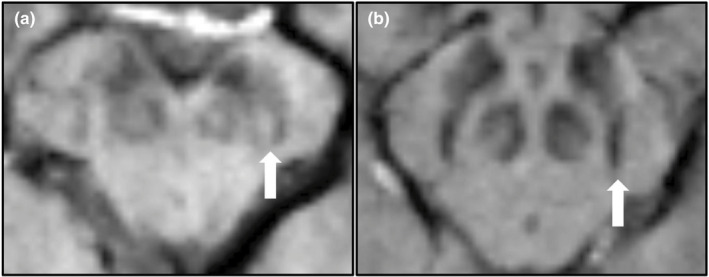
\includegraphics[width=0.8\linewidth]{FileAusiliari/Immagini/degenerative/BRB3-11-e02202-g002}
	\caption{Esempi di segno della coda di rondine (STS) in un individuo malato (a) e di STS assente in un individuo sano (b). Sono mostrate sezioni assiali del mesencefalo mappate tramite imaging pesato con suscettibilità (SWI). Le frecce bianche indicano la diversa configurazione del Nigrosoma-1 (N1). Da Brain Behav. 2021 May 24;11(7):e02202. doi: 10.1002/brb3.2202}
	\label{fig:brb3-11-e02202-g002}
\end{figure*}


La diagnosi differenziale delle sindromi parkinsoniane atipiche beneficia significativamente dell'imaging RM. L'atrofia multisistemica (MSA) evidenzia caratteristica atrofia putaminale, pontica e cerebellare, con ipointensità putaminale T2/SWI e "hot cross bun sign" pontino. La paralisi sopranucleare progressiva (PSP) manifesta atrofia mesencefalica con alterazione del rapporto mesencefalo-ponte, mentre la degenerazione corticobasale (CBD) presenta atrofia frontoparietale asimmetrica con iperintensità della sostanza bianca subcorticale.
Metodiche avanzate quali Diffusion Tensor Imaging (DTI) e risonanza magnetica funzionale (fMRI) consentono la caratterizzazione delle alterazioni microstrutturali della sostanza bianca e delle modificazioni funzionali cerebrali, sebbene la sensibilità nell'identificazione della progressione patologica e nella valutazione della risposta terapeutica necessiti ulteriore validazione. Le limitazioni metodologiche includono variabilità interindividuale e sovrapposizione dei reperti radiologici nelle diverse sindromi parkinsoniane.

\subsection{Trattamento e prognosi}

\subsection{Checklist di refertazione}

\begin{itemize}[label=$\square$] % Riquadro vuoto come simbolo
	\item Escludi altre cause di parkinsonismo (es ictus)
	\item Controlla il segnale dei nigrosomi
	\item Controlla il trofismo delle strutture sottotentoriali
\end{itemize}

\subsection{Bibliografia}
\small{
	
	
}

\note{Nota a margine}
\expl{Nota a margine colorata}
\input{Capitoli/degenerative/approccio.tex}
\input{Capitoli/degenerative/degenerative.tex}
\section{Morbo di Parkinson}

\subsection{Definizione}

\subsection{Eziologia}

\begin{figure*}[h]
	\centering
	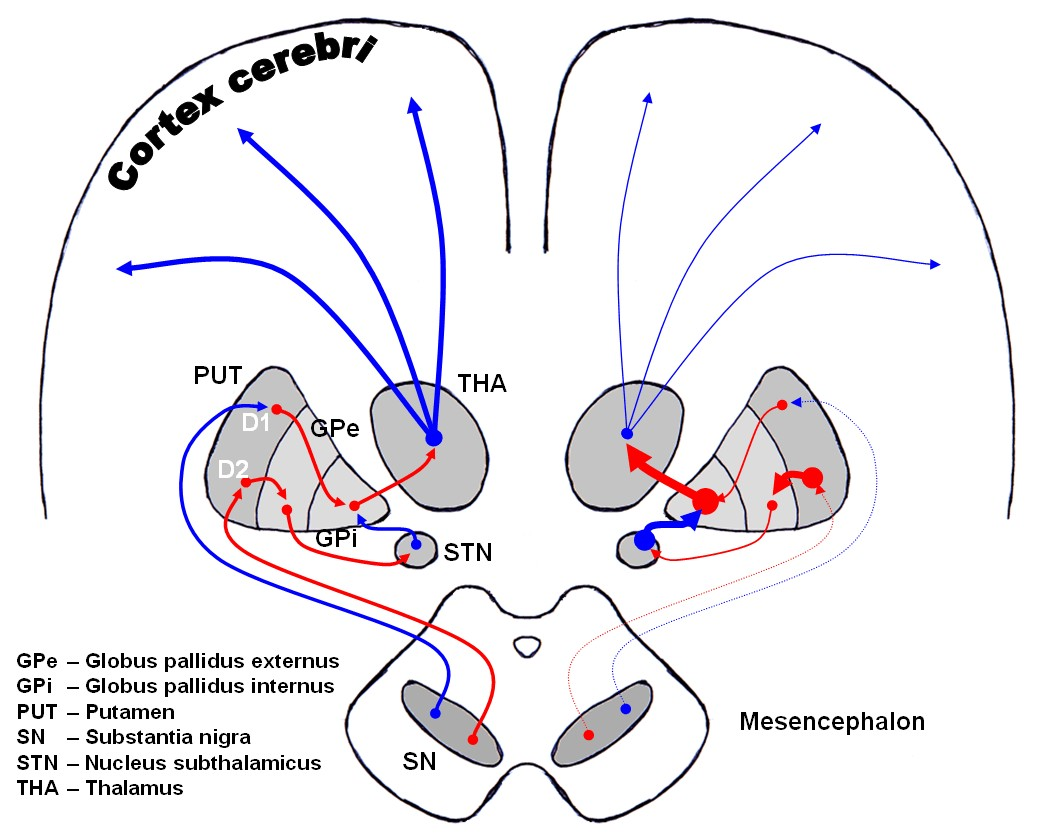
\includegraphics[width=0.5\linewidth]{FileAusiliari/Immagini/degenerative/dopamine-in-parkinsons-disease-illustration}
	\caption[Vie dopaminergiche]{L'immagine mostra le vie dopaminergiche del cervello umano in condizioni normali (a sinistra) e nella malattia di Parkinson (a destra). Le frecce rosse indicano la soppressione del bersaglio, quelle blu la stimolazione della struttura bersaglio. Caso per gentile concessione di Wikipedia, Radiopaedia.org, rID: 36286}
	\label{fig:dopamine-in-parkinsons-disease-illustration}
\end{figure*}

\subsection{Epidemiologia}
Il MP costituisce una delle principali cause di disabilità e mortalità nell'ambito delle patologie neurologiche, con una prevalenza particolarmente elevata negli Stati Uniti e in Canada (160-180 casi/100.000 abitanti). L'incidenza annuale in Nord America oscilla tra 108 e 212 casi ogni 100.000 individui di età $\geq$65 anni, con una prevalenza dello 0,3\% nella popolazione adulta $\geq$40 anni e dell'1,6\% nei soggetti ultrasessantacinquenni.
L'esordio della patologia mostra una significativa correlazione con l'età, manifestandosi tipicamente dalla quinta decade di vita, con un'età media alla diagnosi di 70,5 anni e una finestra di esordio prevalente tra i 45 e i 70 anni. Una variante giovanile può presentarsi tra i 20 e i 40 anni, sebbene l'esordio prima dei 30 anni risulti infrequente. La distribuzione per sesso evidenzia una predominanza maschile, particolarmente accentuata nella fascia d'età 50-60 anni.
L'eziologia del MP comprende fattori di rischio genetici, con particolare rilevanza nelle forme ad esordio precoce, e ambientali, tra cui l'esposizione a pesticidi e inquinanti atmosferici. Sono stati identificati fattori protettivi, inclusi il consumo di caffè, l'attività fisica e il fumo di sigaretta. La patologia si presenta prevalentemente in forma sporadica (85-90\% dei casi), mentre una minoranza dei casi (10-15\%) presenta familiarità positiva.

\subsubsection{Fattori di rischio}
L'eziopatogenesi del Morbo di Parkinson (MP) presenta una complessa interazione di fattori di rischio genetici, ambientali e non modificabili. L'anamnesi familiare positiva per MP in consanguinei di primo grado comporta un incremento del rischio relativo di 2-3 volte. Le forme monogeniche, rappresentanti meno del 10\% della casistica totale, manifestano pattern di ereditarietà autosomica dominante, recessiva o X-linked, caratterizzandosi per un esordio precoce rispetto alle forme sporadiche.
Le mutazioni eterozigoti del gene GBA1 costituiscono un significativo fattore di rischio genetico, unitamente ad alterazioni di altri geni codificanti per enzimi lisosomiali. Il coinvolgimento di geni quali SNCA, LRRK2, VPS35, Parkin, PINK1 e DJ-1 è stato ampiamente documentato. Particolare rilevanza assumono le mutazioni del gene Nurr1, determinante per l'identità neuronale dopaminergica, e del gene DJ-1, cruciale nella risposta allo stress ossidativo. Le alterazioni del gene PINK1, codificante per una chinasi mitocondriale, e del gene Park2, responsabile della sintesi della proteina parkina, sono associate a forme ad esordio precoce.
L'esposizione a neurotossine ambientali, inclusi mercurio, manganese, disolfuro di carbonio, solventi organici, MPTP e monossido di carbonio, può indurre degenerazione nigrostriatale e parkinsonismo. L'uso di neurolettici e l'abuso endovenoso di efedrone possono causare sindromi parkinsoniane potenzialmente irreversibili. Traumi cranici ripetuti, pesticidi, solventi e inquinamento atmosferico rappresentano ulteriori fattori di rischio ambientale documentati.
Tra i fattori non modificabili, l'età avanzata e il sesso maschile emergono come significativi predittori di rischio, con predominanza nella sesta decade di vita. Comorbidità quali depressione, ansia, stipsi, diabete mellito tipo 2, obesità e alterazioni del metabolismo del ferro sono state correlate a un incrementato rischio di MP.
Il consumo di tabacco e caffè, unitamente all'attività fisica regolare, ha mostrato effetti protettivi, sebbene di modesta entità. È fondamentale sottolineare che la maggioranza dei casi di MP rimane idiopatica, suggerendo un'eziologia multifattoriale.

\subsection{Presentazione  clinica}
La sintomatologia del Morbo di Parkinson manifesta un quadro clinico caratterizzato da manifestazioni motorie cardinali e sintomatologia non motoria associata. Il complesso sintomatologico motorio comprende tremore a riposo spesso asimmetrico con frequenza di 4-6 Hz, tipicamente descritto come "pill-rolling", bradicinesia manifestantesi con rallentamento motorio, ipomimia e ridotta oscillazione pendolare degli arti superiori durante la deambulazione, rigidità muscolare ("lead-pipe" o fenomeno della ruota dentata), e instabilità posturale documentabile attraverso il test della retropulsione. La deambulazione risulta caratterizzata da una progressione a piccoli passi con tendenza allo strascicamento e ridotta oscillazione degli arti superiori.
La sintomatologia accessoria include disartria con eloquio esplosivo secondario a incoordinazione linguo-diaframmatica, movimenti involontari della lingua con conseguente difficoltà protrusiva, e incremento della frequenza di ammiccamento palpebrale, quest'ultimo in contrasto con quanto osservato nella corea di Huntington. La disfunzione autonomica, i disturbi olfattivi, la sintomatologia algica, le alterazioni sensitive e i disturbi timici costituiscono il corredo sintomatologico non motorio. Il deterioramento cognitivo, con particolare coinvolgimento delle funzioni attentive, può manifestarsi e progredire nel decorso della patologia.
La progressione temporale della malattia evidenzia un esordio tipicamente unilaterale con successiva bilateralizzazione, manifestandosi prevalentemente nella sesta decade di vita. La responsività alla terapia dopaminergica, in particolare alla levodopa, rappresenta un elemento caratteristico, sebbene il tremore possa risultare farmacoresistente, in contrasto con la significativa risposta della bradicinesia e della rigidità. La variabilità fenotipica interindividuale costituisce un elemento distintivo della patologia.

\subsection{Approccio diagnostico}
L'iter diagnostico della malattia di Parkinson si fonda primariamente sulla valutazione clinica, data l'assenza di biomarcatori patognomonici. La diagnosi richiede la documentazione di bradicinesia associata ad almeno un sintomo cardine tra tremore a riposo o rigidità, valutati mediante la scala MDS-UPDRS standardizzata.
L'approccio diagnostico contempla un'accurata anamnesi ed esame obiettivo neurologico, focalizzati sull'identificazione dei sintomi cardinali: bradicinesia, tremore a riposo (4-6 Hz) tipicamente asimmetrico, rigidità e instabilità posturale. La responsività alla terapia dopaminergica, particolarmente evidente per bradicinesia e rigidità, costituisce un elemento diagnostico supportivo significativo, mentre una mancata risposta a dosaggi adeguati di levodopa suggerisce diagnosi alternative.
L'esclusione di parkinsonismi secondari richiede particolare attenzione all'insorgenza temporale dei sintomi e alla distribuzione topografica del coinvolgimento motorio. La diagnostica per immagini, sebbene non necessaria nelle presentazioni cliniche tipiche con adeguata risposta alla levodopa, può includere RM cerebrale, particolarmente utile mediante sequenze SWI per la valutazione del "swallow tail sign" nigrostriatale. La SPECT con 123I-FP-CIT (DaTscan) documenta la disfunzione dopaminergica presinaptica, mentre la PET con FDG consente la differenziazione metabolica tra PD e sindromi parkinsoniane atipiche.
L'analisi genetica, indicata in casi selezionati (esordio precoce, familiarità positiva, specifiche etnie), e la valutazione autonomica mediante scintigrafia miocardica con MIBG, che evidenzia la denervazione simpatica caratteristica, completano l'iter diagnostico. L'ecografia transcranica può evidenziare l'iperecogenicità della sostanza nera, supportando la diagnosi differenziale.
I criteri MDS stratificano la diagnosi in PD clinicamente stabilita e probabile, bilanciando specificità e sensibilità diagnostica nella pratica clinica.

\begin{Oss}
	La scala MDS-UPDRS (Movement Disorder Society-Unified Parkinson's Disease Rating Scale) è uno strumento di valutazione clinica ampiamente utilizzato per quantificare la gravità dei sintomi motori e non motori della malattia di Parkinson. Questa scala è stata sviluppata per migliorare la consistenza nella valutazione dei sintomi e per integrare meglio gli aspetti non motori della PD.
	Struttura: La scala MDS-UPDRS è composta da quattro sezioni:
	\begin{description}
		\item[Sezione I]{Esperienze non motorie della vita quotidiana. Questa sezione valuta aspetti come le capacità cognitive, i disturbi comportamentali e dell'umore}
		\item [Sezione II]{Esperienze motorie della vita quotidiana. Questa sezione valuta l'impatto dei sintomi motori sulle attività quotidiane}
		\item [Sezione III]{Esame motorio. Questa sezione valuta i segni motori della PD attraverso un esame clinico, come il tremore, la rigidità e la bradicinesia}
		\item[Sezione IV]{Complicanze della terapia. Questa sezione valuta le complicanze associate al trattamento farmacologico}
	\end{description}
	Il punteggio totale per le sezioni I-IV varia da 0 (nessuna disabilità) a 199 (disabilità totale). La sezione III, che valuta i sintomi motori, ha un punteggio che varia da 0 a 132.
	Oltre alla scala MDS-UPDRS, esistono altre scale di valutazione utilizzate nella PD, come la scala di Hoehn e Yahr e la scala di Schwab e England. La scala di Hoehn e Yahr valuta la gravità della malattia da 0 (nessuna malattia) a 5 (paziente costretto su sedia a rotelle o allettato senza assistenza).
\end{Oss}

\subsection{Anatomia patologica}
Dal punto di vista anatomopatologico il morbo di Parkinson si manifesta attraverso inclusioni proteiche intraneuronali denominate corpi di Lewy, costituiti primariamente da aggregati patologici di alfa-sinucleina, una proteina sinaptica fisiologicamente presente nel sistema nervoso centrale. L'accumulo di queste inclusioni, sebbene non patognomonico del morbo di Parkinson essendo documentabile anche nella demenza a corpi di Lewy, rappresenta una caratteristica istopatologica fondamentale quando localizzato nella substantia nigra, in associazione alla perdita neuronale dopaminergica. L'assenza di corpi di Lewy nelle forme post-encefalitiche, caratterizzate invece da grovigli neurofibrillari, e in alcune forme geneticamente determinate, sottolinea l'eterogeneità patogenetica della malattia.
La progressione spazio-temporale della patologia, codificata nello staging di Braak, delinea sei stadi evolutivi caratterizzati da una diffusione ascendente delle alterazioni neuropatologiche. Gli stadi iniziali (1-2) coinvolgono il nucleo motore dorsale dei nervi glossofaringeo e vago e il nucleo olfattivo anteriore, precedendo frequentemente la sintomatologia motoria. Gli stadi intermedi (3-4) documentano il coinvolgimento della substantia nigra pars compacta, del prosencefalo basale e della mesocorteccia temporale, correlando con l'esordio clinico della malattia. Gli stadi terminali (5-6) evidenziano una progressione neocorticale diffusa.
La patogenesi molecolare implica alterazioni del metabolismo dell'alfa-sinucleina, potenzialmente accelerate da disfunzioni delle proteine heat shock o dall'azione della dopamina. Il coinvolgimento della proteina parkin nella degradazione proteasomica evidenzia meccanismi neurodegenerativi potenzialmente indipendenti dalla formazione dei corpi di Lewy.
L'alfa-sinucleina, proteina fisiologicamente localizzata nelle terminazioni presinaptiche neuronali, manifesta nella patogenesi del morbo di Parkinson un processo patologico caratterizzato da misfolding proteico e successiva aggregazione in oligomeri, protofibrille e fibrille, culminante nella formazione dei corpi di Lewy intraneuronali. Questi aggregati proteici, considerati hallmark istopatologico della malattia, evidenziano particolare neurotossicità nella forma protofibrillare, determinando disfunzione e successiva degenerazione neuronale dopaminergica nigrostriatale.
L'identificazione di mutazioni nel gene SNCA, codificante per l'alfa-sinucleina, nelle forme familiari di malattia, unitamente alla documentazione di fenotipi clinici particolarmente aggressivi in presenza di duplicazione o triplicazione genica, ha fornito evidenze significative del ruolo causale di questa proteina nella patogenesi della malattia. La documentata capacità di trasmissione transcellulare dell'alfa-sinucleina patologica costituisce il substrato molecolare della progressione anatomopatologica descritta nello staging di Braak.
La disfunzione sinaptica correlata all'accumulo di alfa-sinucleina rappresenta un meccanismo patogenetico critico, modulato da fattori quali stress ossidativo, alterazioni del sistema ubiquitina-proteasoma e interazione con il metabolismo dopaminergico. Mutazioni nei geni parkin, PINK1 e DJ-1 influenzano il metabolismo dell'alfa-sinucleina attraverso alterazioni dei sistemi di degradazione proteica.
L'alfa-sinucleina costituisce attualmente un promettente target terapeutico, con particolare interesse per lo sviluppo di anticorpi monoclonali specifici e inibitori dell'aggregazione proteica, finalizzati al rallentamento della progressione patologica.

\subsection{Imaging}

\subsubsection{TC}
La TC manifesta un'utilità clinica circoscritta nella valutazione diagnostica primaria del MP, assumendo rilevanza nell'esclusione di patologie strutturali mimiche quali lesioni espansive, idrocefalo o alterazioni vascolari, particolarmente in presenza di presentazioni cliniche atipiche o "red flags" suggestive di diagnosi alternative.
Nel contesto della gestione terapeutica, la TC assume particolare rilevanza nella valutazione post-chirurgica della stimolazione cerebrale profonda (DBS), consentendo la verifica del corretto posizionamento degli elettrodi nel nucleo subtalamico (STN), tipicamente localizzati a 9mm dalla linea mediana, e l'identificazione di eventuali complicanze post-procedurali quali eventi emorragici, ischemici o fenomeni infiammatori transitori, questi ultimi caratterizzati da aree ipodense perilettrodiche a risoluzione graduale. L'utilità della metodica nel follow-up routinario post-DBS risulta secondaria.
La sensibilità subottimale della TC nella diagnosi differenziale tra PD e sindromi parkinsoniane atipiche, incluse atrofia multisistemica e paralisi sopranucleare progressiva, nonché nella distinzione dal tremore essenziale, ne limita significativamente l'applicazione clinica in questo contesto diagnostico.

\subsubsection{RM}
La RM è frequentemente normale nelle sequenze convenzionali (T1, T2, FLAIR) nelle fasi iniziali di malattia. L'implementazione di sequenze susceptibility-weighted imaging (SWI) o T2*-weighted ad alta risoluzione consente la visualizzazione del nigrosoma-1, struttura caratterizzata dal patognomonico "swallow tail sign", la cui perdita correla con la degenerazione dopaminergica nigrostriatale. L'accumulo patologico di ferro nella substantia nigra, quantificabile mediante sequenze SWI/T2* e incrementato del 50\% rispetto ai controlli, costituisce un ulteriore marker diagnostico, complementato dall'imaging della neuromelanina mediante sequenze T1 con impulsi di trasferimento di magnetizzazione (MTC).

\begin{figure*}[h]
	\centering
	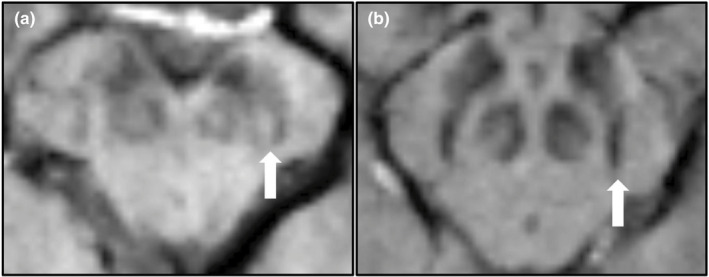
\includegraphics[width=0.8\linewidth]{FileAusiliari/Immagini/degenerative/BRB3-11-e02202-g002}
	\caption{Esempi di segno della coda di rondine (STS) in un individuo malato (a) e di STS assente in un individuo sano (b). Sono mostrate sezioni assiali del mesencefalo mappate tramite imaging pesato con suscettibilità (SWI). Le frecce bianche indicano la diversa configurazione del Nigrosoma-1 (N1). Da Brain Behav. 2021 May 24;11(7):e02202. doi: 10.1002/brb3.2202}
	\label{fig:brb3-11-e02202-g002}
\end{figure*}


La diagnosi differenziale delle sindromi parkinsoniane atipiche beneficia significativamente dell'imaging RM. L'atrofia multisistemica (MSA) evidenzia caratteristica atrofia putaminale, pontica e cerebellare, con ipointensità putaminale T2/SWI e "hot cross bun sign" pontino. La paralisi sopranucleare progressiva (PSP) manifesta atrofia mesencefalica con alterazione del rapporto mesencefalo-ponte, mentre la degenerazione corticobasale (CBD) presenta atrofia frontoparietale asimmetrica con iperintensità della sostanza bianca subcorticale.
Metodiche avanzate quali Diffusion Tensor Imaging (DTI) e risonanza magnetica funzionale (fMRI) consentono la caratterizzazione delle alterazioni microstrutturali della sostanza bianca e delle modificazioni funzionali cerebrali, sebbene la sensibilità nell'identificazione della progressione patologica e nella valutazione della risposta terapeutica necessiti ulteriore validazione. Le limitazioni metodologiche includono variabilità interindividuale e sovrapposizione dei reperti radiologici nelle diverse sindromi parkinsoniane.

\subsection{Trattamento e prognosi}

\subsection{Checklist di refertazione}

\begin{itemize}[label=$\square$] % Riquadro vuoto come simbolo
	\item Escludi altre cause di parkinsonismo (es ictus)
	\item Controlla il segnale dei nigrosomi
	\item Controlla il trofismo delle strutture sottotentoriali
\end{itemize}

\subsection{Bibliografia}
\small{
	
	
}

\note{Nota a margine}
\expl{Nota a margine colorata}
\input{Capitoli/degenerative/approccio.tex}
\input{Capitoli/degenerative/degenerative.tex}
\section{Morbo di Parkinson}

\subsection{Definizione}

\subsection{Eziologia}

\begin{figure*}[h]
	\centering
	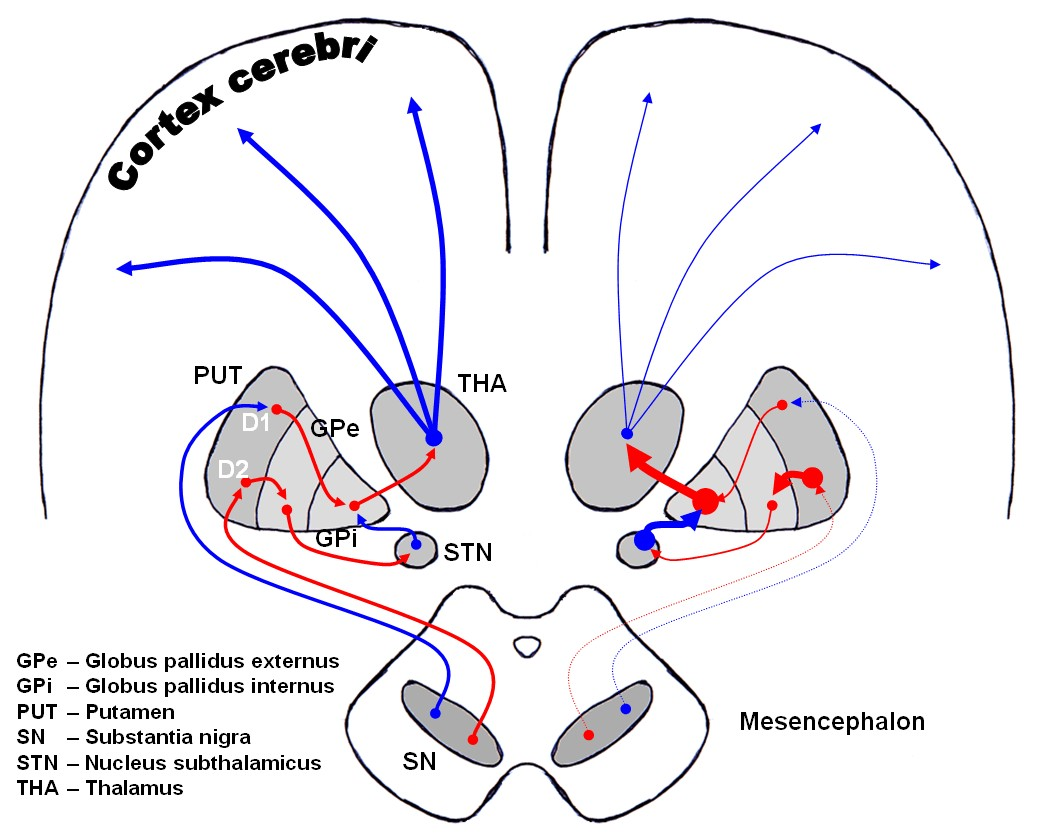
\includegraphics[width=0.5\linewidth]{FileAusiliari/Immagini/degenerative/dopamine-in-parkinsons-disease-illustration}
	\caption[Vie dopaminergiche]{L'immagine mostra le vie dopaminergiche del cervello umano in condizioni normali (a sinistra) e nella malattia di Parkinson (a destra). Le frecce rosse indicano la soppressione del bersaglio, quelle blu la stimolazione della struttura bersaglio. Caso per gentile concessione di Wikipedia, Radiopaedia.org, rID: 36286}
	\label{fig:dopamine-in-parkinsons-disease-illustration}
\end{figure*}

\subsection{Epidemiologia}
Il MP costituisce una delle principali cause di disabilità e mortalità nell'ambito delle patologie neurologiche, con una prevalenza particolarmente elevata negli Stati Uniti e in Canada (160-180 casi/100.000 abitanti). L'incidenza annuale in Nord America oscilla tra 108 e 212 casi ogni 100.000 individui di età $\geq$65 anni, con una prevalenza dello 0,3\% nella popolazione adulta $\geq$40 anni e dell'1,6\% nei soggetti ultrasessantacinquenni.
L'esordio della patologia mostra una significativa correlazione con l'età, manifestandosi tipicamente dalla quinta decade di vita, con un'età media alla diagnosi di 70,5 anni e una finestra di esordio prevalente tra i 45 e i 70 anni. Una variante giovanile può presentarsi tra i 20 e i 40 anni, sebbene l'esordio prima dei 30 anni risulti infrequente. La distribuzione per sesso evidenzia una predominanza maschile, particolarmente accentuata nella fascia d'età 50-60 anni.
L'eziologia del MP comprende fattori di rischio genetici, con particolare rilevanza nelle forme ad esordio precoce, e ambientali, tra cui l'esposizione a pesticidi e inquinanti atmosferici. Sono stati identificati fattori protettivi, inclusi il consumo di caffè, l'attività fisica e il fumo di sigaretta. La patologia si presenta prevalentemente in forma sporadica (85-90\% dei casi), mentre una minoranza dei casi (10-15\%) presenta familiarità positiva.

\subsubsection{Fattori di rischio}
L'eziopatogenesi del Morbo di Parkinson (MP) presenta una complessa interazione di fattori di rischio genetici, ambientali e non modificabili. L'anamnesi familiare positiva per MP in consanguinei di primo grado comporta un incremento del rischio relativo di 2-3 volte. Le forme monogeniche, rappresentanti meno del 10\% della casistica totale, manifestano pattern di ereditarietà autosomica dominante, recessiva o X-linked, caratterizzandosi per un esordio precoce rispetto alle forme sporadiche.
Le mutazioni eterozigoti del gene GBA1 costituiscono un significativo fattore di rischio genetico, unitamente ad alterazioni di altri geni codificanti per enzimi lisosomiali. Il coinvolgimento di geni quali SNCA, LRRK2, VPS35, Parkin, PINK1 e DJ-1 è stato ampiamente documentato. Particolare rilevanza assumono le mutazioni del gene Nurr1, determinante per l'identità neuronale dopaminergica, e del gene DJ-1, cruciale nella risposta allo stress ossidativo. Le alterazioni del gene PINK1, codificante per una chinasi mitocondriale, e del gene Park2, responsabile della sintesi della proteina parkina, sono associate a forme ad esordio precoce.
L'esposizione a neurotossine ambientali, inclusi mercurio, manganese, disolfuro di carbonio, solventi organici, MPTP e monossido di carbonio, può indurre degenerazione nigrostriatale e parkinsonismo. L'uso di neurolettici e l'abuso endovenoso di efedrone possono causare sindromi parkinsoniane potenzialmente irreversibili. Traumi cranici ripetuti, pesticidi, solventi e inquinamento atmosferico rappresentano ulteriori fattori di rischio ambientale documentati.
Tra i fattori non modificabili, l'età avanzata e il sesso maschile emergono come significativi predittori di rischio, con predominanza nella sesta decade di vita. Comorbidità quali depressione, ansia, stipsi, diabete mellito tipo 2, obesità e alterazioni del metabolismo del ferro sono state correlate a un incrementato rischio di MP.
Il consumo di tabacco e caffè, unitamente all'attività fisica regolare, ha mostrato effetti protettivi, sebbene di modesta entità. È fondamentale sottolineare che la maggioranza dei casi di MP rimane idiopatica, suggerendo un'eziologia multifattoriale.

\subsection{Presentazione  clinica}
La sintomatologia del Morbo di Parkinson manifesta un quadro clinico caratterizzato da manifestazioni motorie cardinali e sintomatologia non motoria associata. Il complesso sintomatologico motorio comprende tremore a riposo spesso asimmetrico con frequenza di 4-6 Hz, tipicamente descritto come "pill-rolling", bradicinesia manifestantesi con rallentamento motorio, ipomimia e ridotta oscillazione pendolare degli arti superiori durante la deambulazione, rigidità muscolare ("lead-pipe" o fenomeno della ruota dentata), e instabilità posturale documentabile attraverso il test della retropulsione. La deambulazione risulta caratterizzata da una progressione a piccoli passi con tendenza allo strascicamento e ridotta oscillazione degli arti superiori.
La sintomatologia accessoria include disartria con eloquio esplosivo secondario a incoordinazione linguo-diaframmatica, movimenti involontari della lingua con conseguente difficoltà protrusiva, e incremento della frequenza di ammiccamento palpebrale, quest'ultimo in contrasto con quanto osservato nella corea di Huntington. La disfunzione autonomica, i disturbi olfattivi, la sintomatologia algica, le alterazioni sensitive e i disturbi timici costituiscono il corredo sintomatologico non motorio. Il deterioramento cognitivo, con particolare coinvolgimento delle funzioni attentive, può manifestarsi e progredire nel decorso della patologia.
La progressione temporale della malattia evidenzia un esordio tipicamente unilaterale con successiva bilateralizzazione, manifestandosi prevalentemente nella sesta decade di vita. La responsività alla terapia dopaminergica, in particolare alla levodopa, rappresenta un elemento caratteristico, sebbene il tremore possa risultare farmacoresistente, in contrasto con la significativa risposta della bradicinesia e della rigidità. La variabilità fenotipica interindividuale costituisce un elemento distintivo della patologia.

\subsection{Approccio diagnostico}
L'iter diagnostico della malattia di Parkinson si fonda primariamente sulla valutazione clinica, data l'assenza di biomarcatori patognomonici. La diagnosi richiede la documentazione di bradicinesia associata ad almeno un sintomo cardine tra tremore a riposo o rigidità, valutati mediante la scala MDS-UPDRS standardizzata.
L'approccio diagnostico contempla un'accurata anamnesi ed esame obiettivo neurologico, focalizzati sull'identificazione dei sintomi cardinali: bradicinesia, tremore a riposo (4-6 Hz) tipicamente asimmetrico, rigidità e instabilità posturale. La responsività alla terapia dopaminergica, particolarmente evidente per bradicinesia e rigidità, costituisce un elemento diagnostico supportivo significativo, mentre una mancata risposta a dosaggi adeguati di levodopa suggerisce diagnosi alternative.
L'esclusione di parkinsonismi secondari richiede particolare attenzione all'insorgenza temporale dei sintomi e alla distribuzione topografica del coinvolgimento motorio. La diagnostica per immagini, sebbene non necessaria nelle presentazioni cliniche tipiche con adeguata risposta alla levodopa, può includere RM cerebrale, particolarmente utile mediante sequenze SWI per la valutazione del "swallow tail sign" nigrostriatale. La SPECT con 123I-FP-CIT (DaTscan) documenta la disfunzione dopaminergica presinaptica, mentre la PET con FDG consente la differenziazione metabolica tra PD e sindromi parkinsoniane atipiche.
L'analisi genetica, indicata in casi selezionati (esordio precoce, familiarità positiva, specifiche etnie), e la valutazione autonomica mediante scintigrafia miocardica con MIBG, che evidenzia la denervazione simpatica caratteristica, completano l'iter diagnostico. L'ecografia transcranica può evidenziare l'iperecogenicità della sostanza nera, supportando la diagnosi differenziale.
I criteri MDS stratificano la diagnosi in PD clinicamente stabilita e probabile, bilanciando specificità e sensibilità diagnostica nella pratica clinica.

\begin{Oss}
	La scala MDS-UPDRS (Movement Disorder Society-Unified Parkinson's Disease Rating Scale) è uno strumento di valutazione clinica ampiamente utilizzato per quantificare la gravità dei sintomi motori e non motori della malattia di Parkinson. Questa scala è stata sviluppata per migliorare la consistenza nella valutazione dei sintomi e per integrare meglio gli aspetti non motori della PD.
	Struttura: La scala MDS-UPDRS è composta da quattro sezioni:
	\begin{description}
		\item[Sezione I]{Esperienze non motorie della vita quotidiana. Questa sezione valuta aspetti come le capacità cognitive, i disturbi comportamentali e dell'umore}
		\item [Sezione II]{Esperienze motorie della vita quotidiana. Questa sezione valuta l'impatto dei sintomi motori sulle attività quotidiane}
		\item [Sezione III]{Esame motorio. Questa sezione valuta i segni motori della PD attraverso un esame clinico, come il tremore, la rigidità e la bradicinesia}
		\item[Sezione IV]{Complicanze della terapia. Questa sezione valuta le complicanze associate al trattamento farmacologico}
	\end{description}
	Il punteggio totale per le sezioni I-IV varia da 0 (nessuna disabilità) a 199 (disabilità totale). La sezione III, che valuta i sintomi motori, ha un punteggio che varia da 0 a 132.
	Oltre alla scala MDS-UPDRS, esistono altre scale di valutazione utilizzate nella PD, come la scala di Hoehn e Yahr e la scala di Schwab e England. La scala di Hoehn e Yahr valuta la gravità della malattia da 0 (nessuna malattia) a 5 (paziente costretto su sedia a rotelle o allettato senza assistenza).
\end{Oss}

\subsection{Anatomia patologica}
Dal punto di vista anatomopatologico il morbo di Parkinson si manifesta attraverso inclusioni proteiche intraneuronali denominate corpi di Lewy, costituiti primariamente da aggregati patologici di alfa-sinucleina, una proteina sinaptica fisiologicamente presente nel sistema nervoso centrale. L'accumulo di queste inclusioni, sebbene non patognomonico del morbo di Parkinson essendo documentabile anche nella demenza a corpi di Lewy, rappresenta una caratteristica istopatologica fondamentale quando localizzato nella substantia nigra, in associazione alla perdita neuronale dopaminergica. L'assenza di corpi di Lewy nelle forme post-encefalitiche, caratterizzate invece da grovigli neurofibrillari, e in alcune forme geneticamente determinate, sottolinea l'eterogeneità patogenetica della malattia.
La progressione spazio-temporale della patologia, codificata nello staging di Braak, delinea sei stadi evolutivi caratterizzati da una diffusione ascendente delle alterazioni neuropatologiche. Gli stadi iniziali (1-2) coinvolgono il nucleo motore dorsale dei nervi glossofaringeo e vago e il nucleo olfattivo anteriore, precedendo frequentemente la sintomatologia motoria. Gli stadi intermedi (3-4) documentano il coinvolgimento della substantia nigra pars compacta, del prosencefalo basale e della mesocorteccia temporale, correlando con l'esordio clinico della malattia. Gli stadi terminali (5-6) evidenziano una progressione neocorticale diffusa.
La patogenesi molecolare implica alterazioni del metabolismo dell'alfa-sinucleina, potenzialmente accelerate da disfunzioni delle proteine heat shock o dall'azione della dopamina. Il coinvolgimento della proteina parkin nella degradazione proteasomica evidenzia meccanismi neurodegenerativi potenzialmente indipendenti dalla formazione dei corpi di Lewy.
L'alfa-sinucleina, proteina fisiologicamente localizzata nelle terminazioni presinaptiche neuronali, manifesta nella patogenesi del morbo di Parkinson un processo patologico caratterizzato da misfolding proteico e successiva aggregazione in oligomeri, protofibrille e fibrille, culminante nella formazione dei corpi di Lewy intraneuronali. Questi aggregati proteici, considerati hallmark istopatologico della malattia, evidenziano particolare neurotossicità nella forma protofibrillare, determinando disfunzione e successiva degenerazione neuronale dopaminergica nigrostriatale.
L'identificazione di mutazioni nel gene SNCA, codificante per l'alfa-sinucleina, nelle forme familiari di malattia, unitamente alla documentazione di fenotipi clinici particolarmente aggressivi in presenza di duplicazione o triplicazione genica, ha fornito evidenze significative del ruolo causale di questa proteina nella patogenesi della malattia. La documentata capacità di trasmissione transcellulare dell'alfa-sinucleina patologica costituisce il substrato molecolare della progressione anatomopatologica descritta nello staging di Braak.
La disfunzione sinaptica correlata all'accumulo di alfa-sinucleina rappresenta un meccanismo patogenetico critico, modulato da fattori quali stress ossidativo, alterazioni del sistema ubiquitina-proteasoma e interazione con il metabolismo dopaminergico. Mutazioni nei geni parkin, PINK1 e DJ-1 influenzano il metabolismo dell'alfa-sinucleina attraverso alterazioni dei sistemi di degradazione proteica.
L'alfa-sinucleina costituisce attualmente un promettente target terapeutico, con particolare interesse per lo sviluppo di anticorpi monoclonali specifici e inibitori dell'aggregazione proteica, finalizzati al rallentamento della progressione patologica.

\subsection{Imaging}

\subsubsection{TC}
La TC manifesta un'utilità clinica circoscritta nella valutazione diagnostica primaria del MP, assumendo rilevanza nell'esclusione di patologie strutturali mimiche quali lesioni espansive, idrocefalo o alterazioni vascolari, particolarmente in presenza di presentazioni cliniche atipiche o "red flags" suggestive di diagnosi alternative.
Nel contesto della gestione terapeutica, la TC assume particolare rilevanza nella valutazione post-chirurgica della stimolazione cerebrale profonda (DBS), consentendo la verifica del corretto posizionamento degli elettrodi nel nucleo subtalamico (STN), tipicamente localizzati a 9mm dalla linea mediana, e l'identificazione di eventuali complicanze post-procedurali quali eventi emorragici, ischemici o fenomeni infiammatori transitori, questi ultimi caratterizzati da aree ipodense perilettrodiche a risoluzione graduale. L'utilità della metodica nel follow-up routinario post-DBS risulta secondaria.
La sensibilità subottimale della TC nella diagnosi differenziale tra PD e sindromi parkinsoniane atipiche, incluse atrofia multisistemica e paralisi sopranucleare progressiva, nonché nella distinzione dal tremore essenziale, ne limita significativamente l'applicazione clinica in questo contesto diagnostico.

\subsubsection{RM}
La RM è frequentemente normale nelle sequenze convenzionali (T1, T2, FLAIR) nelle fasi iniziali di malattia. L'implementazione di sequenze susceptibility-weighted imaging (SWI) o T2*-weighted ad alta risoluzione consente la visualizzazione del nigrosoma-1, struttura caratterizzata dal patognomonico "swallow tail sign", la cui perdita correla con la degenerazione dopaminergica nigrostriatale. L'accumulo patologico di ferro nella substantia nigra, quantificabile mediante sequenze SWI/T2* e incrementato del 50\% rispetto ai controlli, costituisce un ulteriore marker diagnostico, complementato dall'imaging della neuromelanina mediante sequenze T1 con impulsi di trasferimento di magnetizzazione (MTC).

\begin{figure*}[h]
	\centering
	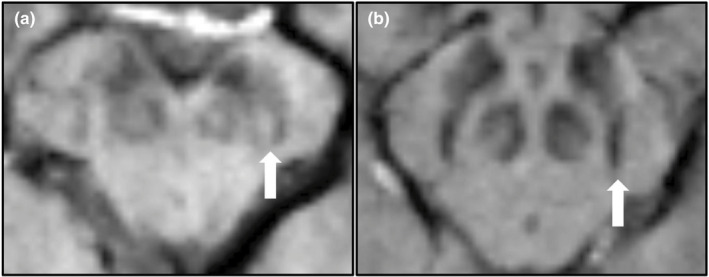
\includegraphics[width=0.8\linewidth]{FileAusiliari/Immagini/degenerative/BRB3-11-e02202-g002}
	\caption{Esempi di segno della coda di rondine (STS) in un individuo malato (a) e di STS assente in un individuo sano (b). Sono mostrate sezioni assiali del mesencefalo mappate tramite imaging pesato con suscettibilità (SWI). Le frecce bianche indicano la diversa configurazione del Nigrosoma-1 (N1). Da Brain Behav. 2021 May 24;11(7):e02202. doi: 10.1002/brb3.2202}
	\label{fig:brb3-11-e02202-g002}
\end{figure*}


La diagnosi differenziale delle sindromi parkinsoniane atipiche beneficia significativamente dell'imaging RM. L'atrofia multisistemica (MSA) evidenzia caratteristica atrofia putaminale, pontica e cerebellare, con ipointensità putaminale T2/SWI e "hot cross bun sign" pontino. La paralisi sopranucleare progressiva (PSP) manifesta atrofia mesencefalica con alterazione del rapporto mesencefalo-ponte, mentre la degenerazione corticobasale (CBD) presenta atrofia frontoparietale asimmetrica con iperintensità della sostanza bianca subcorticale.
Metodiche avanzate quali Diffusion Tensor Imaging (DTI) e risonanza magnetica funzionale (fMRI) consentono la caratterizzazione delle alterazioni microstrutturali della sostanza bianca e delle modificazioni funzionali cerebrali, sebbene la sensibilità nell'identificazione della progressione patologica e nella valutazione della risposta terapeutica necessiti ulteriore validazione. Le limitazioni metodologiche includono variabilità interindividuale e sovrapposizione dei reperti radiologici nelle diverse sindromi parkinsoniane.

\subsection{Trattamento e prognosi}

\subsection{Checklist di refertazione}

\begin{itemize}[label=$\square$] % Riquadro vuoto come simbolo
	\item Escludi altre cause di parkinsonismo (es ictus)
	\item Controlla il segnale dei nigrosomi
	\item Controlla il trofismo delle strutture sottotentoriali
\end{itemize}

\subsection{Bibliografia}
\small{
	
	
}

\note{Nota a margine}
\expl{Nota a margine colorata}
\input{Capitoli/degenerative/approccio.tex}
\input{Capitoli/degenerative/degenerative.tex}
\section{Morbo di Parkinson}

\subsection{Definizione}

\subsection{Eziologia}

\begin{figure*}[h]
	\centering
	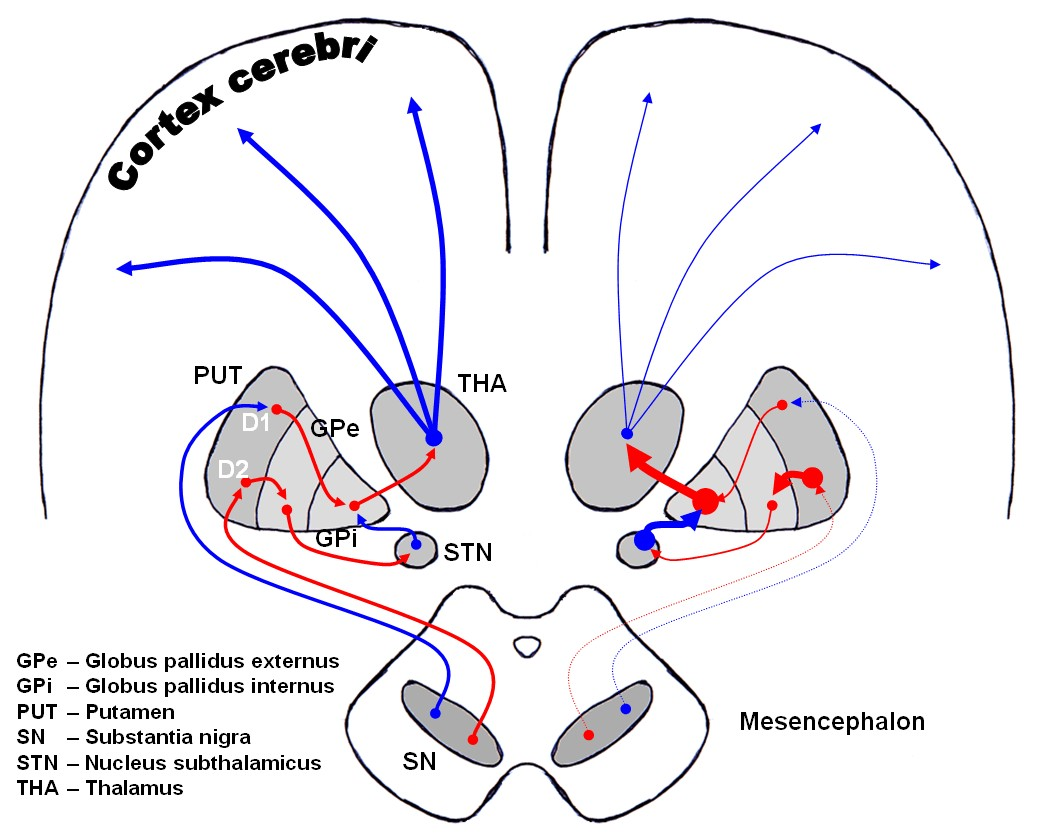
\includegraphics[width=0.5\linewidth]{FileAusiliari/Immagini/degenerative/dopamine-in-parkinsons-disease-illustration}
	\caption[Vie dopaminergiche]{L'immagine mostra le vie dopaminergiche del cervello umano in condizioni normali (a sinistra) e nella malattia di Parkinson (a destra). Le frecce rosse indicano la soppressione del bersaglio, quelle blu la stimolazione della struttura bersaglio. Caso per gentile concessione di Wikipedia, Radiopaedia.org, rID: 36286}
	\label{fig:dopamine-in-parkinsons-disease-illustration}
\end{figure*}

\subsection{Epidemiologia}
Il MP costituisce una delle principali cause di disabilità e mortalità nell'ambito delle patologie neurologiche, con una prevalenza particolarmente elevata negli Stati Uniti e in Canada (160-180 casi/100.000 abitanti). L'incidenza annuale in Nord America oscilla tra 108 e 212 casi ogni 100.000 individui di età $\geq$65 anni, con una prevalenza dello 0,3\% nella popolazione adulta $\geq$40 anni e dell'1,6\% nei soggetti ultrasessantacinquenni.
L'esordio della patologia mostra una significativa correlazione con l'età, manifestandosi tipicamente dalla quinta decade di vita, con un'età media alla diagnosi di 70,5 anni e una finestra di esordio prevalente tra i 45 e i 70 anni. Una variante giovanile può presentarsi tra i 20 e i 40 anni, sebbene l'esordio prima dei 30 anni risulti infrequente. La distribuzione per sesso evidenzia una predominanza maschile, particolarmente accentuata nella fascia d'età 50-60 anni.
L'eziologia del MP comprende fattori di rischio genetici, con particolare rilevanza nelle forme ad esordio precoce, e ambientali, tra cui l'esposizione a pesticidi e inquinanti atmosferici. Sono stati identificati fattori protettivi, inclusi il consumo di caffè, l'attività fisica e il fumo di sigaretta. La patologia si presenta prevalentemente in forma sporadica (85-90\% dei casi), mentre una minoranza dei casi (10-15\%) presenta familiarità positiva.

\subsubsection{Fattori di rischio}
L'eziopatogenesi del Morbo di Parkinson (MP) presenta una complessa interazione di fattori di rischio genetici, ambientali e non modificabili. L'anamnesi familiare positiva per MP in consanguinei di primo grado comporta un incremento del rischio relativo di 2-3 volte. Le forme monogeniche, rappresentanti meno del 10\% della casistica totale, manifestano pattern di ereditarietà autosomica dominante, recessiva o X-linked, caratterizzandosi per un esordio precoce rispetto alle forme sporadiche.
Le mutazioni eterozigoti del gene GBA1 costituiscono un significativo fattore di rischio genetico, unitamente ad alterazioni di altri geni codificanti per enzimi lisosomiali. Il coinvolgimento di geni quali SNCA, LRRK2, VPS35, Parkin, PINK1 e DJ-1 è stato ampiamente documentato. Particolare rilevanza assumono le mutazioni del gene Nurr1, determinante per l'identità neuronale dopaminergica, e del gene DJ-1, cruciale nella risposta allo stress ossidativo. Le alterazioni del gene PINK1, codificante per una chinasi mitocondriale, e del gene Park2, responsabile della sintesi della proteina parkina, sono associate a forme ad esordio precoce.
L'esposizione a neurotossine ambientali, inclusi mercurio, manganese, disolfuro di carbonio, solventi organici, MPTP e monossido di carbonio, può indurre degenerazione nigrostriatale e parkinsonismo. L'uso di neurolettici e l'abuso endovenoso di efedrone possono causare sindromi parkinsoniane potenzialmente irreversibili. Traumi cranici ripetuti, pesticidi, solventi e inquinamento atmosferico rappresentano ulteriori fattori di rischio ambientale documentati.
Tra i fattori non modificabili, l'età avanzata e il sesso maschile emergono come significativi predittori di rischio, con predominanza nella sesta decade di vita. Comorbidità quali depressione, ansia, stipsi, diabete mellito tipo 2, obesità e alterazioni del metabolismo del ferro sono state correlate a un incrementato rischio di MP.
Il consumo di tabacco e caffè, unitamente all'attività fisica regolare, ha mostrato effetti protettivi, sebbene di modesta entità. È fondamentale sottolineare che la maggioranza dei casi di MP rimane idiopatica, suggerendo un'eziologia multifattoriale.

\subsection{Presentazione  clinica}
La sintomatologia del Morbo di Parkinson manifesta un quadro clinico caratterizzato da manifestazioni motorie cardinali e sintomatologia non motoria associata. Il complesso sintomatologico motorio comprende tremore a riposo spesso asimmetrico con frequenza di 4-6 Hz, tipicamente descritto come "pill-rolling", bradicinesia manifestantesi con rallentamento motorio, ipomimia e ridotta oscillazione pendolare degli arti superiori durante la deambulazione, rigidità muscolare ("lead-pipe" o fenomeno della ruota dentata), e instabilità posturale documentabile attraverso il test della retropulsione. La deambulazione risulta caratterizzata da una progressione a piccoli passi con tendenza allo strascicamento e ridotta oscillazione degli arti superiori.
La sintomatologia accessoria include disartria con eloquio esplosivo secondario a incoordinazione linguo-diaframmatica, movimenti involontari della lingua con conseguente difficoltà protrusiva, e incremento della frequenza di ammiccamento palpebrale, quest'ultimo in contrasto con quanto osservato nella corea di Huntington. La disfunzione autonomica, i disturbi olfattivi, la sintomatologia algica, le alterazioni sensitive e i disturbi timici costituiscono il corredo sintomatologico non motorio. Il deterioramento cognitivo, con particolare coinvolgimento delle funzioni attentive, può manifestarsi e progredire nel decorso della patologia.
La progressione temporale della malattia evidenzia un esordio tipicamente unilaterale con successiva bilateralizzazione, manifestandosi prevalentemente nella sesta decade di vita. La responsività alla terapia dopaminergica, in particolare alla levodopa, rappresenta un elemento caratteristico, sebbene il tremore possa risultare farmacoresistente, in contrasto con la significativa risposta della bradicinesia e della rigidità. La variabilità fenotipica interindividuale costituisce un elemento distintivo della patologia.

\subsection{Approccio diagnostico}
L'iter diagnostico della malattia di Parkinson si fonda primariamente sulla valutazione clinica, data l'assenza di biomarcatori patognomonici. La diagnosi richiede la documentazione di bradicinesia associata ad almeno un sintomo cardine tra tremore a riposo o rigidità, valutati mediante la scala MDS-UPDRS standardizzata.
L'approccio diagnostico contempla un'accurata anamnesi ed esame obiettivo neurologico, focalizzati sull'identificazione dei sintomi cardinali: bradicinesia, tremore a riposo (4-6 Hz) tipicamente asimmetrico, rigidità e instabilità posturale. La responsività alla terapia dopaminergica, particolarmente evidente per bradicinesia e rigidità, costituisce un elemento diagnostico supportivo significativo, mentre una mancata risposta a dosaggi adeguati di levodopa suggerisce diagnosi alternative.
L'esclusione di parkinsonismi secondari richiede particolare attenzione all'insorgenza temporale dei sintomi e alla distribuzione topografica del coinvolgimento motorio. La diagnostica per immagini, sebbene non necessaria nelle presentazioni cliniche tipiche con adeguata risposta alla levodopa, può includere RM cerebrale, particolarmente utile mediante sequenze SWI per la valutazione del "swallow tail sign" nigrostriatale. La SPECT con 123I-FP-CIT (DaTscan) documenta la disfunzione dopaminergica presinaptica, mentre la PET con FDG consente la differenziazione metabolica tra PD e sindromi parkinsoniane atipiche.
L'analisi genetica, indicata in casi selezionati (esordio precoce, familiarità positiva, specifiche etnie), e la valutazione autonomica mediante scintigrafia miocardica con MIBG, che evidenzia la denervazione simpatica caratteristica, completano l'iter diagnostico. L'ecografia transcranica può evidenziare l'iperecogenicità della sostanza nera, supportando la diagnosi differenziale.
I criteri MDS stratificano la diagnosi in PD clinicamente stabilita e probabile, bilanciando specificità e sensibilità diagnostica nella pratica clinica.

\begin{Oss}
	La scala MDS-UPDRS (Movement Disorder Society-Unified Parkinson's Disease Rating Scale) è uno strumento di valutazione clinica ampiamente utilizzato per quantificare la gravità dei sintomi motori e non motori della malattia di Parkinson. Questa scala è stata sviluppata per migliorare la consistenza nella valutazione dei sintomi e per integrare meglio gli aspetti non motori della PD.
	Struttura: La scala MDS-UPDRS è composta da quattro sezioni:
	\begin{description}
		\item[Sezione I]{Esperienze non motorie della vita quotidiana. Questa sezione valuta aspetti come le capacità cognitive, i disturbi comportamentali e dell'umore}
		\item [Sezione II]{Esperienze motorie della vita quotidiana. Questa sezione valuta l'impatto dei sintomi motori sulle attività quotidiane}
		\item [Sezione III]{Esame motorio. Questa sezione valuta i segni motori della PD attraverso un esame clinico, come il tremore, la rigidità e la bradicinesia}
		\item[Sezione IV]{Complicanze della terapia. Questa sezione valuta le complicanze associate al trattamento farmacologico}
	\end{description}
	Il punteggio totale per le sezioni I-IV varia da 0 (nessuna disabilità) a 199 (disabilità totale). La sezione III, che valuta i sintomi motori, ha un punteggio che varia da 0 a 132.
	Oltre alla scala MDS-UPDRS, esistono altre scale di valutazione utilizzate nella PD, come la scala di Hoehn e Yahr e la scala di Schwab e England. La scala di Hoehn e Yahr valuta la gravità della malattia da 0 (nessuna malattia) a 5 (paziente costretto su sedia a rotelle o allettato senza assistenza).
\end{Oss}

\subsection{Anatomia patologica}
Dal punto di vista anatomopatologico il morbo di Parkinson si manifesta attraverso inclusioni proteiche intraneuronali denominate corpi di Lewy, costituiti primariamente da aggregati patologici di alfa-sinucleina, una proteina sinaptica fisiologicamente presente nel sistema nervoso centrale. L'accumulo di queste inclusioni, sebbene non patognomonico del morbo di Parkinson essendo documentabile anche nella demenza a corpi di Lewy, rappresenta una caratteristica istopatologica fondamentale quando localizzato nella substantia nigra, in associazione alla perdita neuronale dopaminergica. L'assenza di corpi di Lewy nelle forme post-encefalitiche, caratterizzate invece da grovigli neurofibrillari, e in alcune forme geneticamente determinate, sottolinea l'eterogeneità patogenetica della malattia.
La progressione spazio-temporale della patologia, codificata nello staging di Braak, delinea sei stadi evolutivi caratterizzati da una diffusione ascendente delle alterazioni neuropatologiche. Gli stadi iniziali (1-2) coinvolgono il nucleo motore dorsale dei nervi glossofaringeo e vago e il nucleo olfattivo anteriore, precedendo frequentemente la sintomatologia motoria. Gli stadi intermedi (3-4) documentano il coinvolgimento della substantia nigra pars compacta, del prosencefalo basale e della mesocorteccia temporale, correlando con l'esordio clinico della malattia. Gli stadi terminali (5-6) evidenziano una progressione neocorticale diffusa.
La patogenesi molecolare implica alterazioni del metabolismo dell'alfa-sinucleina, potenzialmente accelerate da disfunzioni delle proteine heat shock o dall'azione della dopamina. Il coinvolgimento della proteina parkin nella degradazione proteasomica evidenzia meccanismi neurodegenerativi potenzialmente indipendenti dalla formazione dei corpi di Lewy.
L'alfa-sinucleina, proteina fisiologicamente localizzata nelle terminazioni presinaptiche neuronali, manifesta nella patogenesi del morbo di Parkinson un processo patologico caratterizzato da misfolding proteico e successiva aggregazione in oligomeri, protofibrille e fibrille, culminante nella formazione dei corpi di Lewy intraneuronali. Questi aggregati proteici, considerati hallmark istopatologico della malattia, evidenziano particolare neurotossicità nella forma protofibrillare, determinando disfunzione e successiva degenerazione neuronale dopaminergica nigrostriatale.
L'identificazione di mutazioni nel gene SNCA, codificante per l'alfa-sinucleina, nelle forme familiari di malattia, unitamente alla documentazione di fenotipi clinici particolarmente aggressivi in presenza di duplicazione o triplicazione genica, ha fornito evidenze significative del ruolo causale di questa proteina nella patogenesi della malattia. La documentata capacità di trasmissione transcellulare dell'alfa-sinucleina patologica costituisce il substrato molecolare della progressione anatomopatologica descritta nello staging di Braak.
La disfunzione sinaptica correlata all'accumulo di alfa-sinucleina rappresenta un meccanismo patogenetico critico, modulato da fattori quali stress ossidativo, alterazioni del sistema ubiquitina-proteasoma e interazione con il metabolismo dopaminergico. Mutazioni nei geni parkin, PINK1 e DJ-1 influenzano il metabolismo dell'alfa-sinucleina attraverso alterazioni dei sistemi di degradazione proteica.
L'alfa-sinucleina costituisce attualmente un promettente target terapeutico, con particolare interesse per lo sviluppo di anticorpi monoclonali specifici e inibitori dell'aggregazione proteica, finalizzati al rallentamento della progressione patologica.

\subsection{Imaging}

\subsubsection{TC}
La TC manifesta un'utilità clinica circoscritta nella valutazione diagnostica primaria del MP, assumendo rilevanza nell'esclusione di patologie strutturali mimiche quali lesioni espansive, idrocefalo o alterazioni vascolari, particolarmente in presenza di presentazioni cliniche atipiche o "red flags" suggestive di diagnosi alternative.
Nel contesto della gestione terapeutica, la TC assume particolare rilevanza nella valutazione post-chirurgica della stimolazione cerebrale profonda (DBS), consentendo la verifica del corretto posizionamento degli elettrodi nel nucleo subtalamico (STN), tipicamente localizzati a 9mm dalla linea mediana, e l'identificazione di eventuali complicanze post-procedurali quali eventi emorragici, ischemici o fenomeni infiammatori transitori, questi ultimi caratterizzati da aree ipodense perilettrodiche a risoluzione graduale. L'utilità della metodica nel follow-up routinario post-DBS risulta secondaria.
La sensibilità subottimale della TC nella diagnosi differenziale tra PD e sindromi parkinsoniane atipiche, incluse atrofia multisistemica e paralisi sopranucleare progressiva, nonché nella distinzione dal tremore essenziale, ne limita significativamente l'applicazione clinica in questo contesto diagnostico.

\subsubsection{RM}
La RM è frequentemente normale nelle sequenze convenzionali (T1, T2, FLAIR) nelle fasi iniziali di malattia. L'implementazione di sequenze susceptibility-weighted imaging (SWI) o T2*-weighted ad alta risoluzione consente la visualizzazione del nigrosoma-1, struttura caratterizzata dal patognomonico "swallow tail sign", la cui perdita correla con la degenerazione dopaminergica nigrostriatale. L'accumulo patologico di ferro nella substantia nigra, quantificabile mediante sequenze SWI/T2* e incrementato del 50\% rispetto ai controlli, costituisce un ulteriore marker diagnostico, complementato dall'imaging della neuromelanina mediante sequenze T1 con impulsi di trasferimento di magnetizzazione (MTC).

\begin{figure*}[h]
	\centering
	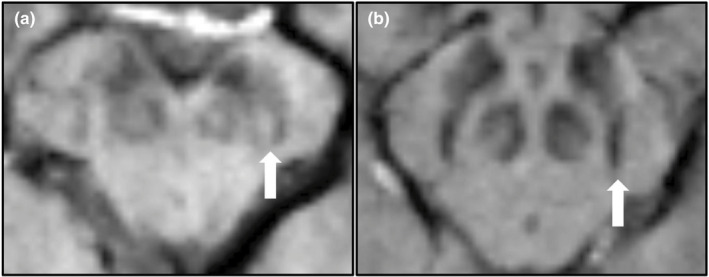
\includegraphics[width=0.8\linewidth]{FileAusiliari/Immagini/degenerative/BRB3-11-e02202-g002}
	\caption{Esempi di segno della coda di rondine (STS) in un individuo malato (a) e di STS assente in un individuo sano (b). Sono mostrate sezioni assiali del mesencefalo mappate tramite imaging pesato con suscettibilità (SWI). Le frecce bianche indicano la diversa configurazione del Nigrosoma-1 (N1). Da Brain Behav. 2021 May 24;11(7):e02202. doi: 10.1002/brb3.2202}
	\label{fig:brb3-11-e02202-g002}
\end{figure*}


La diagnosi differenziale delle sindromi parkinsoniane atipiche beneficia significativamente dell'imaging RM. L'atrofia multisistemica (MSA) evidenzia caratteristica atrofia putaminale, pontica e cerebellare, con ipointensità putaminale T2/SWI e "hot cross bun sign" pontino. La paralisi sopranucleare progressiva (PSP) manifesta atrofia mesencefalica con alterazione del rapporto mesencefalo-ponte, mentre la degenerazione corticobasale (CBD) presenta atrofia frontoparietale asimmetrica con iperintensità della sostanza bianca subcorticale.
Metodiche avanzate quali Diffusion Tensor Imaging (DTI) e risonanza magnetica funzionale (fMRI) consentono la caratterizzazione delle alterazioni microstrutturali della sostanza bianca e delle modificazioni funzionali cerebrali, sebbene la sensibilità nell'identificazione della progressione patologica e nella valutazione della risposta terapeutica necessiti ulteriore validazione. Le limitazioni metodologiche includono variabilità interindividuale e sovrapposizione dei reperti radiologici nelle diverse sindromi parkinsoniane.

\subsection{Trattamento e prognosi}

\subsection{Checklist di refertazione}

\begin{itemize}[label=$\square$] % Riquadro vuoto come simbolo
	\item Escludi altre cause di parkinsonismo (es ictus)
	\item Controlla il segnale dei nigrosomi
	\item Controlla il trofismo delle strutture sottotentoriali
\end{itemize}

\subsection{Bibliografia}
\small{
	
	
}

\note{Nota a margine}
\expl{Nota a margine colorata}
\input{Capitoli/degenerative/approccio.tex}
\input{Capitoli/degenerative/degenerative.tex}
\section{Morbo di Parkinson}

\subsection{Definizione}

\subsection{Eziologia}

\begin{figure*}[h]
	\centering
	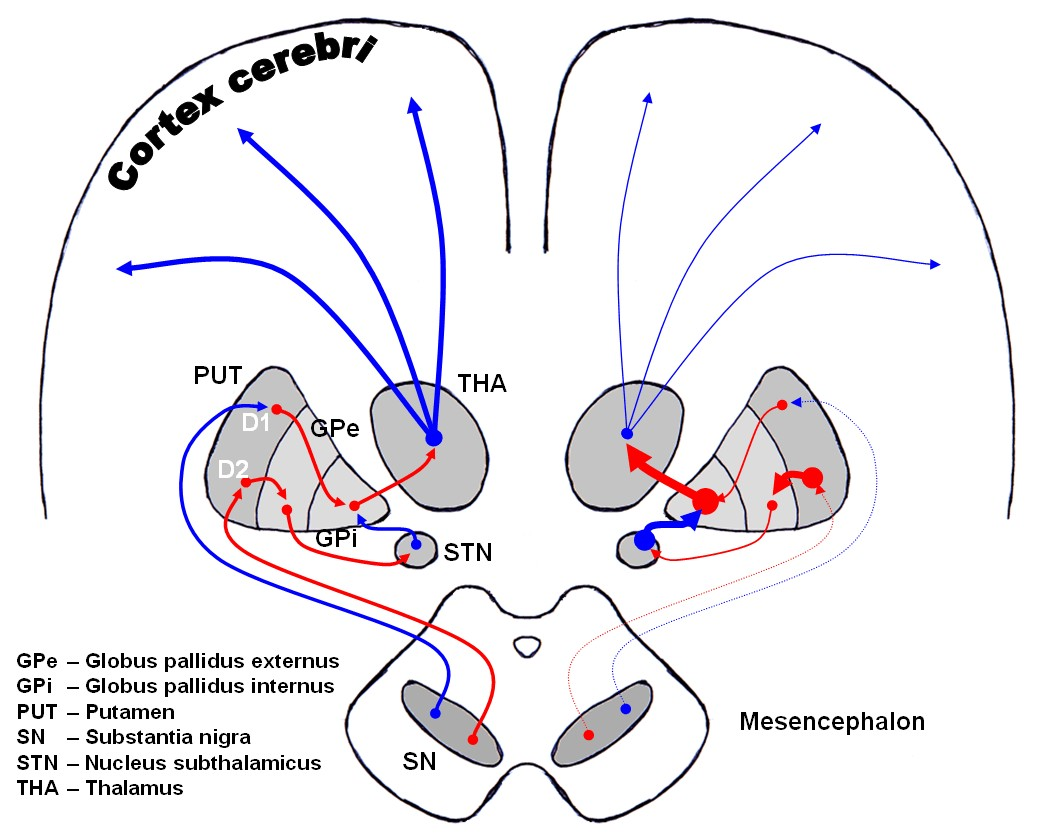
\includegraphics[width=0.5\linewidth]{FileAusiliari/Immagini/degenerative/dopamine-in-parkinsons-disease-illustration}
	\caption[Vie dopaminergiche]{L'immagine mostra le vie dopaminergiche del cervello umano in condizioni normali (a sinistra) e nella malattia di Parkinson (a destra). Le frecce rosse indicano la soppressione del bersaglio, quelle blu la stimolazione della struttura bersaglio. Caso per gentile concessione di Wikipedia, Radiopaedia.org, rID: 36286}
	\label{fig:dopamine-in-parkinsons-disease-illustration}
\end{figure*}

\subsection{Epidemiologia}
Il MP costituisce una delle principali cause di disabilità e mortalità nell'ambito delle patologie neurologiche, con una prevalenza particolarmente elevata negli Stati Uniti e in Canada (160-180 casi/100.000 abitanti). L'incidenza annuale in Nord America oscilla tra 108 e 212 casi ogni 100.000 individui di età $\geq$65 anni, con una prevalenza dello 0,3\% nella popolazione adulta $\geq$40 anni e dell'1,6\% nei soggetti ultrasessantacinquenni.
L'esordio della patologia mostra una significativa correlazione con l'età, manifestandosi tipicamente dalla quinta decade di vita, con un'età media alla diagnosi di 70,5 anni e una finestra di esordio prevalente tra i 45 e i 70 anni. Una variante giovanile può presentarsi tra i 20 e i 40 anni, sebbene l'esordio prima dei 30 anni risulti infrequente. La distribuzione per sesso evidenzia una predominanza maschile, particolarmente accentuata nella fascia d'età 50-60 anni.
L'eziologia del MP comprende fattori di rischio genetici, con particolare rilevanza nelle forme ad esordio precoce, e ambientali, tra cui l'esposizione a pesticidi e inquinanti atmosferici. Sono stati identificati fattori protettivi, inclusi il consumo di caffè, l'attività fisica e il fumo di sigaretta. La patologia si presenta prevalentemente in forma sporadica (85-90\% dei casi), mentre una minoranza dei casi (10-15\%) presenta familiarità positiva.

\subsubsection{Fattori di rischio}
L'eziopatogenesi del Morbo di Parkinson (MP) presenta una complessa interazione di fattori di rischio genetici, ambientali e non modificabili. L'anamnesi familiare positiva per MP in consanguinei di primo grado comporta un incremento del rischio relativo di 2-3 volte. Le forme monogeniche, rappresentanti meno del 10\% della casistica totale, manifestano pattern di ereditarietà autosomica dominante, recessiva o X-linked, caratterizzandosi per un esordio precoce rispetto alle forme sporadiche.
Le mutazioni eterozigoti del gene GBA1 costituiscono un significativo fattore di rischio genetico, unitamente ad alterazioni di altri geni codificanti per enzimi lisosomiali. Il coinvolgimento di geni quali SNCA, LRRK2, VPS35, Parkin, PINK1 e DJ-1 è stato ampiamente documentato. Particolare rilevanza assumono le mutazioni del gene Nurr1, determinante per l'identità neuronale dopaminergica, e del gene DJ-1, cruciale nella risposta allo stress ossidativo. Le alterazioni del gene PINK1, codificante per una chinasi mitocondriale, e del gene Park2, responsabile della sintesi della proteina parkina, sono associate a forme ad esordio precoce.
L'esposizione a neurotossine ambientali, inclusi mercurio, manganese, disolfuro di carbonio, solventi organici, MPTP e monossido di carbonio, può indurre degenerazione nigrostriatale e parkinsonismo. L'uso di neurolettici e l'abuso endovenoso di efedrone possono causare sindromi parkinsoniane potenzialmente irreversibili. Traumi cranici ripetuti, pesticidi, solventi e inquinamento atmosferico rappresentano ulteriori fattori di rischio ambientale documentati.
Tra i fattori non modificabili, l'età avanzata e il sesso maschile emergono come significativi predittori di rischio, con predominanza nella sesta decade di vita. Comorbidità quali depressione, ansia, stipsi, diabete mellito tipo 2, obesità e alterazioni del metabolismo del ferro sono state correlate a un incrementato rischio di MP.
Il consumo di tabacco e caffè, unitamente all'attività fisica regolare, ha mostrato effetti protettivi, sebbene di modesta entità. È fondamentale sottolineare che la maggioranza dei casi di MP rimane idiopatica, suggerendo un'eziologia multifattoriale.

\subsection{Presentazione  clinica}
La sintomatologia del Morbo di Parkinson manifesta un quadro clinico caratterizzato da manifestazioni motorie cardinali e sintomatologia non motoria associata. Il complesso sintomatologico motorio comprende tremore a riposo spesso asimmetrico con frequenza di 4-6 Hz, tipicamente descritto come "pill-rolling", bradicinesia manifestantesi con rallentamento motorio, ipomimia e ridotta oscillazione pendolare degli arti superiori durante la deambulazione, rigidità muscolare ("lead-pipe" o fenomeno della ruota dentata), e instabilità posturale documentabile attraverso il test della retropulsione. La deambulazione risulta caratterizzata da una progressione a piccoli passi con tendenza allo strascicamento e ridotta oscillazione degli arti superiori.
La sintomatologia accessoria include disartria con eloquio esplosivo secondario a incoordinazione linguo-diaframmatica, movimenti involontari della lingua con conseguente difficoltà protrusiva, e incremento della frequenza di ammiccamento palpebrale, quest'ultimo in contrasto con quanto osservato nella corea di Huntington. La disfunzione autonomica, i disturbi olfattivi, la sintomatologia algica, le alterazioni sensitive e i disturbi timici costituiscono il corredo sintomatologico non motorio. Il deterioramento cognitivo, con particolare coinvolgimento delle funzioni attentive, può manifestarsi e progredire nel decorso della patologia.
La progressione temporale della malattia evidenzia un esordio tipicamente unilaterale con successiva bilateralizzazione, manifestandosi prevalentemente nella sesta decade di vita. La responsività alla terapia dopaminergica, in particolare alla levodopa, rappresenta un elemento caratteristico, sebbene il tremore possa risultare farmacoresistente, in contrasto con la significativa risposta della bradicinesia e della rigidità. La variabilità fenotipica interindividuale costituisce un elemento distintivo della patologia.

\subsection{Approccio diagnostico}
L'iter diagnostico della malattia di Parkinson si fonda primariamente sulla valutazione clinica, data l'assenza di biomarcatori patognomonici. La diagnosi richiede la documentazione di bradicinesia associata ad almeno un sintomo cardine tra tremore a riposo o rigidità, valutati mediante la scala MDS-UPDRS standardizzata.
L'approccio diagnostico contempla un'accurata anamnesi ed esame obiettivo neurologico, focalizzati sull'identificazione dei sintomi cardinali: bradicinesia, tremore a riposo (4-6 Hz) tipicamente asimmetrico, rigidità e instabilità posturale. La responsività alla terapia dopaminergica, particolarmente evidente per bradicinesia e rigidità, costituisce un elemento diagnostico supportivo significativo, mentre una mancata risposta a dosaggi adeguati di levodopa suggerisce diagnosi alternative.
L'esclusione di parkinsonismi secondari richiede particolare attenzione all'insorgenza temporale dei sintomi e alla distribuzione topografica del coinvolgimento motorio. La diagnostica per immagini, sebbene non necessaria nelle presentazioni cliniche tipiche con adeguata risposta alla levodopa, può includere RM cerebrale, particolarmente utile mediante sequenze SWI per la valutazione del "swallow tail sign" nigrostriatale. La SPECT con 123I-FP-CIT (DaTscan) documenta la disfunzione dopaminergica presinaptica, mentre la PET con FDG consente la differenziazione metabolica tra PD e sindromi parkinsoniane atipiche.
L'analisi genetica, indicata in casi selezionati (esordio precoce, familiarità positiva, specifiche etnie), e la valutazione autonomica mediante scintigrafia miocardica con MIBG, che evidenzia la denervazione simpatica caratteristica, completano l'iter diagnostico. L'ecografia transcranica può evidenziare l'iperecogenicità della sostanza nera, supportando la diagnosi differenziale.
I criteri MDS stratificano la diagnosi in PD clinicamente stabilita e probabile, bilanciando specificità e sensibilità diagnostica nella pratica clinica.

\begin{Oss}
	La scala MDS-UPDRS (Movement Disorder Society-Unified Parkinson's Disease Rating Scale) è uno strumento di valutazione clinica ampiamente utilizzato per quantificare la gravità dei sintomi motori e non motori della malattia di Parkinson. Questa scala è stata sviluppata per migliorare la consistenza nella valutazione dei sintomi e per integrare meglio gli aspetti non motori della PD.
	Struttura: La scala MDS-UPDRS è composta da quattro sezioni:
	\begin{description}
		\item[Sezione I]{Esperienze non motorie della vita quotidiana. Questa sezione valuta aspetti come le capacità cognitive, i disturbi comportamentali e dell'umore}
		\item [Sezione II]{Esperienze motorie della vita quotidiana. Questa sezione valuta l'impatto dei sintomi motori sulle attività quotidiane}
		\item [Sezione III]{Esame motorio. Questa sezione valuta i segni motori della PD attraverso un esame clinico, come il tremore, la rigidità e la bradicinesia}
		\item[Sezione IV]{Complicanze della terapia. Questa sezione valuta le complicanze associate al trattamento farmacologico}
	\end{description}
	Il punteggio totale per le sezioni I-IV varia da 0 (nessuna disabilità) a 199 (disabilità totale). La sezione III, che valuta i sintomi motori, ha un punteggio che varia da 0 a 132.
	Oltre alla scala MDS-UPDRS, esistono altre scale di valutazione utilizzate nella PD, come la scala di Hoehn e Yahr e la scala di Schwab e England. La scala di Hoehn e Yahr valuta la gravità della malattia da 0 (nessuna malattia) a 5 (paziente costretto su sedia a rotelle o allettato senza assistenza).
\end{Oss}

\subsection{Anatomia patologica}
Dal punto di vista anatomopatologico il morbo di Parkinson si manifesta attraverso inclusioni proteiche intraneuronali denominate corpi di Lewy, costituiti primariamente da aggregati patologici di alfa-sinucleina, una proteina sinaptica fisiologicamente presente nel sistema nervoso centrale. L'accumulo di queste inclusioni, sebbene non patognomonico del morbo di Parkinson essendo documentabile anche nella demenza a corpi di Lewy, rappresenta una caratteristica istopatologica fondamentale quando localizzato nella substantia nigra, in associazione alla perdita neuronale dopaminergica. L'assenza di corpi di Lewy nelle forme post-encefalitiche, caratterizzate invece da grovigli neurofibrillari, e in alcune forme geneticamente determinate, sottolinea l'eterogeneità patogenetica della malattia.
La progressione spazio-temporale della patologia, codificata nello staging di Braak, delinea sei stadi evolutivi caratterizzati da una diffusione ascendente delle alterazioni neuropatologiche. Gli stadi iniziali (1-2) coinvolgono il nucleo motore dorsale dei nervi glossofaringeo e vago e il nucleo olfattivo anteriore, precedendo frequentemente la sintomatologia motoria. Gli stadi intermedi (3-4) documentano il coinvolgimento della substantia nigra pars compacta, del prosencefalo basale e della mesocorteccia temporale, correlando con l'esordio clinico della malattia. Gli stadi terminali (5-6) evidenziano una progressione neocorticale diffusa.
La patogenesi molecolare implica alterazioni del metabolismo dell'alfa-sinucleina, potenzialmente accelerate da disfunzioni delle proteine heat shock o dall'azione della dopamina. Il coinvolgimento della proteina parkin nella degradazione proteasomica evidenzia meccanismi neurodegenerativi potenzialmente indipendenti dalla formazione dei corpi di Lewy.
L'alfa-sinucleina, proteina fisiologicamente localizzata nelle terminazioni presinaptiche neuronali, manifesta nella patogenesi del morbo di Parkinson un processo patologico caratterizzato da misfolding proteico e successiva aggregazione in oligomeri, protofibrille e fibrille, culminante nella formazione dei corpi di Lewy intraneuronali. Questi aggregati proteici, considerati hallmark istopatologico della malattia, evidenziano particolare neurotossicità nella forma protofibrillare, determinando disfunzione e successiva degenerazione neuronale dopaminergica nigrostriatale.
L'identificazione di mutazioni nel gene SNCA, codificante per l'alfa-sinucleina, nelle forme familiari di malattia, unitamente alla documentazione di fenotipi clinici particolarmente aggressivi in presenza di duplicazione o triplicazione genica, ha fornito evidenze significative del ruolo causale di questa proteina nella patogenesi della malattia. La documentata capacità di trasmissione transcellulare dell'alfa-sinucleina patologica costituisce il substrato molecolare della progressione anatomopatologica descritta nello staging di Braak.
La disfunzione sinaptica correlata all'accumulo di alfa-sinucleina rappresenta un meccanismo patogenetico critico, modulato da fattori quali stress ossidativo, alterazioni del sistema ubiquitina-proteasoma e interazione con il metabolismo dopaminergico. Mutazioni nei geni parkin, PINK1 e DJ-1 influenzano il metabolismo dell'alfa-sinucleina attraverso alterazioni dei sistemi di degradazione proteica.
L'alfa-sinucleina costituisce attualmente un promettente target terapeutico, con particolare interesse per lo sviluppo di anticorpi monoclonali specifici e inibitori dell'aggregazione proteica, finalizzati al rallentamento della progressione patologica.

\subsection{Imaging}

\subsubsection{TC}
La TC manifesta un'utilità clinica circoscritta nella valutazione diagnostica primaria del MP, assumendo rilevanza nell'esclusione di patologie strutturali mimiche quali lesioni espansive, idrocefalo o alterazioni vascolari, particolarmente in presenza di presentazioni cliniche atipiche o "red flags" suggestive di diagnosi alternative.
Nel contesto della gestione terapeutica, la TC assume particolare rilevanza nella valutazione post-chirurgica della stimolazione cerebrale profonda (DBS), consentendo la verifica del corretto posizionamento degli elettrodi nel nucleo subtalamico (STN), tipicamente localizzati a 9mm dalla linea mediana, e l'identificazione di eventuali complicanze post-procedurali quali eventi emorragici, ischemici o fenomeni infiammatori transitori, questi ultimi caratterizzati da aree ipodense perilettrodiche a risoluzione graduale. L'utilità della metodica nel follow-up routinario post-DBS risulta secondaria.
La sensibilità subottimale della TC nella diagnosi differenziale tra PD e sindromi parkinsoniane atipiche, incluse atrofia multisistemica e paralisi sopranucleare progressiva, nonché nella distinzione dal tremore essenziale, ne limita significativamente l'applicazione clinica in questo contesto diagnostico.

\subsubsection{RM}
La RM è frequentemente normale nelle sequenze convenzionali (T1, T2, FLAIR) nelle fasi iniziali di malattia. L'implementazione di sequenze susceptibility-weighted imaging (SWI) o T2*-weighted ad alta risoluzione consente la visualizzazione del nigrosoma-1, struttura caratterizzata dal patognomonico "swallow tail sign", la cui perdita correla con la degenerazione dopaminergica nigrostriatale. L'accumulo patologico di ferro nella substantia nigra, quantificabile mediante sequenze SWI/T2* e incrementato del 50\% rispetto ai controlli, costituisce un ulteriore marker diagnostico, complementato dall'imaging della neuromelanina mediante sequenze T1 con impulsi di trasferimento di magnetizzazione (MTC).

\begin{figure*}[h]
	\centering
	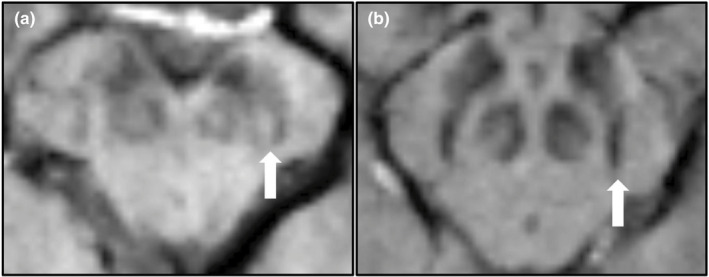
\includegraphics[width=0.8\linewidth]{FileAusiliari/Immagini/degenerative/BRB3-11-e02202-g002}
	\caption{Esempi di segno della coda di rondine (STS) in un individuo malato (a) e di STS assente in un individuo sano (b). Sono mostrate sezioni assiali del mesencefalo mappate tramite imaging pesato con suscettibilità (SWI). Le frecce bianche indicano la diversa configurazione del Nigrosoma-1 (N1). Da Brain Behav. 2021 May 24;11(7):e02202. doi: 10.1002/brb3.2202}
	\label{fig:brb3-11-e02202-g002}
\end{figure*}


La diagnosi differenziale delle sindromi parkinsoniane atipiche beneficia significativamente dell'imaging RM. L'atrofia multisistemica (MSA) evidenzia caratteristica atrofia putaminale, pontica e cerebellare, con ipointensità putaminale T2/SWI e "hot cross bun sign" pontino. La paralisi sopranucleare progressiva (PSP) manifesta atrofia mesencefalica con alterazione del rapporto mesencefalo-ponte, mentre la degenerazione corticobasale (CBD) presenta atrofia frontoparietale asimmetrica con iperintensità della sostanza bianca subcorticale.
Metodiche avanzate quali Diffusion Tensor Imaging (DTI) e risonanza magnetica funzionale (fMRI) consentono la caratterizzazione delle alterazioni microstrutturali della sostanza bianca e delle modificazioni funzionali cerebrali, sebbene la sensibilità nell'identificazione della progressione patologica e nella valutazione della risposta terapeutica necessiti ulteriore validazione. Le limitazioni metodologiche includono variabilità interindividuale e sovrapposizione dei reperti radiologici nelle diverse sindromi parkinsoniane.

\subsection{Trattamento e prognosi}

\subsection{Checklist di refertazione}

\begin{itemize}[label=$\square$] % Riquadro vuoto come simbolo
	\item Escludi altre cause di parkinsonismo (es ictus)
	\item Controlla il segnale dei nigrosomi
	\item Controlla il trofismo delle strutture sottotentoriali
\end{itemize}

\subsection{Bibliografia}
\small{
	
	
}

\note{Nota a margine}
\expl{Nota a margine colorata}

%%%%%								APPENDICI
\newgeometry{top=35mm, bottom=35mm, left=15mm, right=15mm, headheight=0pt, headsep=0pt, marginparsep=0pt, marginparwidth=0pt, footskip=0pt, footnotesep=0pt}
\part*{\HUGE Appendici}
\titleformat{\chapter}[display]    	{\bfseries\large\raggedright}    	{\vspace{-2.35cm} \MakeUppercase{\chaptertitlename}\ \Huge \thechapter}    	{.125ex}    	{\raggedleft\vspace{-1cm}\Huge\makebox[.5\textwidth]{}}
\titlespacing*{\chapter}{0pt}{6\baselineskip}{2.5\baselineskip}
\restoregeometry

	% Capitoli
\titlecontents{chapter}[2.5pc]
{\addvspace{15pt}}
{\begin{tikzpicture}
		\pgftext{\LArge\bfseries\bfseries\color{black}\hspace{-1cm} Appendice\ \thecontentslabel{\color{white}.}\hspace{.5cm} }
	\end{tikzpicture}\Large }
{}
{\color{black}\titlerule\; \;\Large\bfseries Pagina \thecontentspage}

\pagestyle{fancyapp}

\begin{appendices}
	\chapter{Titolo}\label{AppendiceA}
	\blindduck[maths]


%%%%%%%%%%%%%%%%%%%%%%%%%%%%									BACKMATTER
%%%%%%%%%%%%%%%%%%%%%%%%%%%%
\backmatter

%%%%% 							BIBLIOGRAFIA
\pagestyle{fancyBibliografia}
\titleformat{\chapter}
	[hang]
	{\vspace{-2cm}\Huge}
	{}
	{0em}
	{}
	[\Large {\begin{tikzpicture} [remember picture, overlay]
	\pgftext[right,x=14.75cm,y=0.2cm]{\HUGE\bfseries 
	Bibliografia}
	\end{tikzpicture}}]
	
	\nocite{*}
	\bibliographystyle{amsalpha}
	\bibliography{FileAusiliari/Bibliografia}
	\addcontentsline{toc}{part}{Bibliografia}
\cleardoublepage
%INDICE ANALITICO
 \pagestyle{fancyIndiceAnalitico}
 	\renewcommand{\indexname}{}
	% SISTEMA IL PROBLEMA DEL LINK ALL'INDICE ANALITICO
	\let\cleardoublepage\relax
	\titleformat{\chapter}[hang]{}{}{0em}{}[]
 	\chapter*{}
	\titleformat{\chapter}
		[hang]
		{\Huge}
		{}
		{0em}
		{}
		[\Large {\begin{tikzpicture} [remember picture, overlay]
		\pgftext[right,x=14.75cm,y=0.2cm]{\HUGE\bfseries 
			Indice analitico}
		\end{tikzpicture}}]
	\titlespacing*{\chapter}{0pt}{0\baselineskip}{5\baselineskip}
	\addcontentsline{toc}{part}{Indice analitico}	
	\vspace{-2cm}
	\printindex
%%%%%%%%%%%%%%%%%%%%%%%%%%%%%%%%%%%%%%%%%%%%%%%%%%%%%%%%%%%%%%%%%%%%%%%%%%%%%%%%%%%%%%%%%%%%%%%%%%%%%%%%%%%%%%%%%
\end{appendices}
\end{document}